% Options for packages loaded elsewhere
\PassOptionsToPackage{unicode}{hyperref}
\PassOptionsToPackage{hyphens}{url}
%
\documentclass[
]{book}
\usepackage{amsmath,amssymb}
\usepackage{lmodern}
\usepackage{ifxetex,ifluatex}
\ifnum 0\ifxetex 1\fi\ifluatex 1\fi=0 % if pdftex
  \usepackage[T1]{fontenc}
  \usepackage[utf8]{inputenc}
  \usepackage{textcomp} % provide euro and other symbols
\else % if luatex or xetex
  \usepackage{unicode-math}
  \defaultfontfeatures{Scale=MatchLowercase}
  \defaultfontfeatures[\rmfamily]{Ligatures=TeX,Scale=1}
\fi
% Use upquote if available, for straight quotes in verbatim environments
\IfFileExists{upquote.sty}{\usepackage{upquote}}{}
\IfFileExists{microtype.sty}{% use microtype if available
  \usepackage[]{microtype}
  \UseMicrotypeSet[protrusion]{basicmath} % disable protrusion for tt fonts
}{}
\makeatletter
\@ifundefined{KOMAClassName}{% if non-KOMA class
  \IfFileExists{parskip.sty}{%
    \usepackage{parskip}
  }{% else
    \setlength{\parindent}{0pt}
    \setlength{\parskip}{6pt plus 2pt minus 1pt}}
}{% if KOMA class
  \KOMAoptions{parskip=half}}
\makeatother
\usepackage{xcolor}
\IfFileExists{xurl.sty}{\usepackage{xurl}}{} % add URL line breaks if available
\IfFileExists{bookmark.sty}{\usepackage{bookmark}}{\usepackage{hyperref}}
\hypersetup{
  pdftitle={Introdução ao Ambiente R de Programação},
  pdfauthor={Fabio Cop; fabiocopf@gmail.com; Instituto do Mar, Universidade Federal de São Paulo},
  hidelinks,
  pdfcreator={LaTeX via pandoc}}
\urlstyle{same} % disable monospaced font for URLs
\usepackage{color}
\usepackage{fancyvrb}
\newcommand{\VerbBar}{|}
\newcommand{\VERB}{\Verb[commandchars=\\\{\}]}
\DefineVerbatimEnvironment{Highlighting}{Verbatim}{commandchars=\\\{\}}
% Add ',fontsize=\small' for more characters per line
\usepackage{framed}
\definecolor{shadecolor}{RGB}{248,248,248}
\newenvironment{Shaded}{\begin{snugshade}}{\end{snugshade}}
\newcommand{\AlertTok}[1]{\textcolor[rgb]{0.94,0.16,0.16}{#1}}
\newcommand{\AnnotationTok}[1]{\textcolor[rgb]{0.56,0.35,0.01}{\textbf{\textit{#1}}}}
\newcommand{\AttributeTok}[1]{\textcolor[rgb]{0.77,0.63,0.00}{#1}}
\newcommand{\BaseNTok}[1]{\textcolor[rgb]{0.00,0.00,0.81}{#1}}
\newcommand{\BuiltInTok}[1]{#1}
\newcommand{\CharTok}[1]{\textcolor[rgb]{0.31,0.60,0.02}{#1}}
\newcommand{\CommentTok}[1]{\textcolor[rgb]{0.56,0.35,0.01}{\textit{#1}}}
\newcommand{\CommentVarTok}[1]{\textcolor[rgb]{0.56,0.35,0.01}{\textbf{\textit{#1}}}}
\newcommand{\ConstantTok}[1]{\textcolor[rgb]{0.00,0.00,0.00}{#1}}
\newcommand{\ControlFlowTok}[1]{\textcolor[rgb]{0.13,0.29,0.53}{\textbf{#1}}}
\newcommand{\DataTypeTok}[1]{\textcolor[rgb]{0.13,0.29,0.53}{#1}}
\newcommand{\DecValTok}[1]{\textcolor[rgb]{0.00,0.00,0.81}{#1}}
\newcommand{\DocumentationTok}[1]{\textcolor[rgb]{0.56,0.35,0.01}{\textbf{\textit{#1}}}}
\newcommand{\ErrorTok}[1]{\textcolor[rgb]{0.64,0.00,0.00}{\textbf{#1}}}
\newcommand{\ExtensionTok}[1]{#1}
\newcommand{\FloatTok}[1]{\textcolor[rgb]{0.00,0.00,0.81}{#1}}
\newcommand{\FunctionTok}[1]{\textcolor[rgb]{0.00,0.00,0.00}{#1}}
\newcommand{\ImportTok}[1]{#1}
\newcommand{\InformationTok}[1]{\textcolor[rgb]{0.56,0.35,0.01}{\textbf{\textit{#1}}}}
\newcommand{\KeywordTok}[1]{\textcolor[rgb]{0.13,0.29,0.53}{\textbf{#1}}}
\newcommand{\NormalTok}[1]{#1}
\newcommand{\OperatorTok}[1]{\textcolor[rgb]{0.81,0.36,0.00}{\textbf{#1}}}
\newcommand{\OtherTok}[1]{\textcolor[rgb]{0.56,0.35,0.01}{#1}}
\newcommand{\PreprocessorTok}[1]{\textcolor[rgb]{0.56,0.35,0.01}{\textit{#1}}}
\newcommand{\RegionMarkerTok}[1]{#1}
\newcommand{\SpecialCharTok}[1]{\textcolor[rgb]{0.00,0.00,0.00}{#1}}
\newcommand{\SpecialStringTok}[1]{\textcolor[rgb]{0.31,0.60,0.02}{#1}}
\newcommand{\StringTok}[1]{\textcolor[rgb]{0.31,0.60,0.02}{#1}}
\newcommand{\VariableTok}[1]{\textcolor[rgb]{0.00,0.00,0.00}{#1}}
\newcommand{\VerbatimStringTok}[1]{\textcolor[rgb]{0.31,0.60,0.02}{#1}}
\newcommand{\WarningTok}[1]{\textcolor[rgb]{0.56,0.35,0.01}{\textbf{\textit{#1}}}}
\usepackage{longtable,booktabs,array}
\usepackage{calc} % for calculating minipage widths
% Correct order of tables after \paragraph or \subparagraph
\usepackage{etoolbox}
\makeatletter
\patchcmd\longtable{\par}{\if@noskipsec\mbox{}\fi\par}{}{}
\makeatother
% Allow footnotes in longtable head/foot
\IfFileExists{footnotehyper.sty}{\usepackage{footnotehyper}}{\usepackage{footnote}}
\makesavenoteenv{longtable}
\usepackage{graphicx}
\makeatletter
\def\maxwidth{\ifdim\Gin@nat@width>\linewidth\linewidth\else\Gin@nat@width\fi}
\def\maxheight{\ifdim\Gin@nat@height>\textheight\textheight\else\Gin@nat@height\fi}
\makeatother
% Scale images if necessary, so that they will not overflow the page
% margins by default, and it is still possible to overwrite the defaults
% using explicit options in \includegraphics[width, height, ...]{}
\setkeys{Gin}{width=\maxwidth,height=\maxheight,keepaspectratio}
% Set default figure placement to htbp
\makeatletter
\def\fps@figure{htbp}
\makeatother
\setlength{\emergencystretch}{3em} % prevent overfull lines
\providecommand{\tightlist}{%
  \setlength{\itemsep}{0pt}\setlength{\parskip}{0pt}}
\setcounter{secnumdepth}{5}
\usepackage{booktabs}
\usepackage{amsthm}
\makeatletter
\def\thm@space@setup{%
  \thm@preskip=8pt plus 2pt minus 4pt
  \thm@postskip=\thm@preskip
}
\makeatother
\ifluatex
  \usepackage{selnolig}  % disable illegal ligatures
\fi
\usepackage[]{natbib}
\bibliographystyle{apalike}

\title{Introdução ao Ambiente R de Programação}
\author{Fabio Cop \and \href{mailto:fabiocopf@gmail.com}{\nolinkurl{fabiocopf@gmail.com}} \and Instituto do Mar, Universidade Federal de São Paulo}
\date{2021-05-18}

\begin{document}
\maketitle

{
\setcounter{tocdepth}{1}
\tableofcontents
}
\hypertarget{apresentauxe7uxe3o}{%
\chapter*{Apresentação}\label{apresentauxe7uxe3o}}
\addcontentsline{toc}{chapter}{Apresentação}

Este é um material de introdução sobre o ambiente de programação R. O material está dividido em duas partes: I. Fundamentos de programação em R (capítulos \ref{intro} a \ref{visualizacao}) e II. Uma coleção integrada de pacotes para ciência de dados (capítulos \ref{tidy} a \ref{ggplot2}).

\hypertarget{part-fundamentos-de-programauxe7uxe3o-em-r}{%
\part{Fundamentos de programação em R}\label{part-fundamentos-de-programauxe7uxe3o-em-r}}

\hypertarget{intro}{%
\chapter{Introdução ao programa R}\label{intro}}

O R é um ambiente de análise de dados, cálculos matemáticos, análises estatísticas e apresentação gráfica. É um programa livre e de código aberto com aplicações nas mais diversas áreas das ciências. Para informações sobre o programa acesse a página oficial do R \href{https://www.r-project.org/}{https://www.r-project.org}, onde existe uma extensa variedade de informações, apostilas e área de download para as plataformas Linux, Windows e MacOS. Outras fontes de informação são o R-blogers \href{https://www.r-bloggers.com/}{https://www.r-bloggers.com}, o \href{https://pt.stackoverflow.com/}{stackoverflow}, \href{https://towardsdatascience.com/}{towards data science} ou ainda inúmeras páginas, tutoriais, videos e apostilas que podem ser encontrados em uma busca no \href{https://www.google.com.br/}{Google}. Neste capítulo faremos uma breve introdução ao R e, no capítulo seguinte, abordaremos tópicos sobre maniupulação e visualização de dados.

\hypertarget{instalauxe7uxe3o-do-r}{%
\section{Instalação do R}\label{instalauxe7uxe3o-do-r}}

O R pode ser instalado a partir do site oficial \href{https://cran.r-project.org/}{CRAN}. A instalação em ambiente Windows pode ser obtida no link \texttt{Download\ R\ for\ Windows\ -\/-\textgreater{}\ base} onde você irá encontrar a versão mais atual disponível para seu sistema. Em ambiente Mac OS X a instalação pode ser feita a partir do link \texttt{Download\ R\ for\ (Mac)\ OS\ X} buscando pelo pacote \texttt{.pkg}. Para ambiente Linux, entre no link \texttt{Download\ R\ for\ Linux} e escolha sua plataforma (Ubuntu, Debian, Fedora, etc.). Nela você poderá obter as instruções de instalação.

\hypertarget{interface-de-desenvolvimento-ide}{%
\section{Interface de desenvolvimento (IDE)}\label{interface-de-desenvolvimento-ide}}

Uma IDE (\emph{Integrated Development Environment}) é um ambiente de desenvolvimento integrado, que faciliatm o uso de linguagens de programação. Existe uma variedade de IDE's para programação em R. Você pode pesquisar por estas opções na internet e buscar por aquela que melhor atenda suas necessidades. Resalto duas opções utilizadas no contexto de análise de dados, estatística e ciência de dados: o \href{https://rstudio.com/}{RStudio} e o \href{https://jupyter.org/index.html}{Jupyter Notebook}.

O RStudio é um ambiente intregrado ao R, embora também seja utilizado para desenvolvimento em outras linguagens de programação. Por ter sido desenvivido primariamente para desenvolvimento em R, ofecere uma grande variedade de opções, desde a simples visualização de dados até a instalação e manutenção de pacotes. Esta será a interface que iremos utilizar para dar sequência a este material.

A instalação do RStudio pode ser feita em ambiente Windos, MAC OS X e Linux. A instalação em Windows e MAC OS X seguem o caminho tradicional de instalação de programas nestes ambientes. Em Linux você poderá encontrar uma variedade de tutoriais para a sua plataforma.

A vantagem do Jupyter Notebook é sua estrutura simples que facilita a curva de aprendizado. Atualmente (2021-05-18) é mais utilizado para desenvolvimento e análise de dados em \href{https://www.python.org/}{Python}, porém você poderá encontrar facilmente tutoriais para configuração do ambiente em R.

\hypertarget{o-r-para-cuxe1lculos-aritmuxe9ticos}{%
\section{O R para cálculos aritméticos}\label{o-r-para-cuxe1lculos-aritmuxe9ticos}}

Vamos iniciar nossa introdução ao R com seu uso mais simples, um ambiente para cálculos aritméticos. Como você verá, o R usa os operadores matemáticos de subtração (\texttt{-}), adição (\texttt{+}), multiplicação (\texttt{*}), divisão (\texttt{/}) e potenciação (\texttt{\^{}}) do modo análogo a outros softwares.

\begin{Shaded}
\begin{Highlighting}[]
\DecValTok{2} \SpecialCharTok{+} \DecValTok{4}
\end{Highlighting}
\end{Shaded}

\begin{verbatim}
## [1] 6
\end{verbatim}

\begin{Shaded}
\begin{Highlighting}[]
\DecValTok{2} \SpecialCharTok{*} \DecValTok{4}
\end{Highlighting}
\end{Shaded}

\begin{verbatim}
## [1] 8
\end{verbatim}

\begin{Shaded}
\begin{Highlighting}[]
\DecValTok{2} \SpecialCharTok{{-}} \DecValTok{4}
\end{Highlighting}
\end{Shaded}

\begin{verbatim}
## [1] -2
\end{verbatim}

\begin{Shaded}
\begin{Highlighting}[]
\DecValTok{2}\SpecialCharTok{\^{}}\DecValTok{4}
\end{Highlighting}
\end{Shaded}

\begin{verbatim}
## [1] 16
\end{verbatim}

Além destes, temos operadores para extrairmos a parte inteira (\texttt{\%\%}) e o resto (\texttt{\%/\%}) de uma divisão.

\begin{Shaded}
\begin{Highlighting}[]
\DecValTok{13}\SpecialCharTok{\%/\%}\DecValTok{2}
\end{Highlighting}
\end{Shaded}

\begin{verbatim}
## [1] 6
\end{verbatim}

\begin{Shaded}
\begin{Highlighting}[]
\DecValTok{13}\SpecialCharTok{\%\%}\DecValTok{2}
\end{Highlighting}
\end{Shaded}

\begin{verbatim}
## [1] 1
\end{verbatim}

O uso de parênteses também permite o controle das operações matemáticas seguindo as prioridades conhecidas nestas operações. Por exemplo, a expressão:

\begin{Shaded}
\begin{Highlighting}[]
\DecValTok{5} \SpecialCharTok{*}\NormalTok{ (}\DecValTok{9} \SpecialCharTok{+} \DecValTok{2}\NormalTok{)}
\end{Highlighting}
\end{Shaded}

\begin{verbatim}
## [1] 55
\end{verbatim}

é diferente de:

\begin{Shaded}
\begin{Highlighting}[]
\DecValTok{5} \SpecialCharTok{*} \DecValTok{9} \SpecialCharTok{+} \DecValTok{2}
\end{Highlighting}
\end{Shaded}

\begin{verbatim}
## [1] 47
\end{verbatim}

Assim como a expressão:

\begin{Shaded}
\begin{Highlighting}[]
\NormalTok{(}\DecValTok{3} \SpecialCharTok{+} \DecValTok{4}\NormalTok{)}\SpecialCharTok{\^{}}\DecValTok{2}
\end{Highlighting}
\end{Shaded}

\begin{verbatim}
## [1] 49
\end{verbatim}

é diferente de:

\begin{Shaded}
\begin{Highlighting}[]
\DecValTok{3} \SpecialCharTok{+} \DecValTok{4}\SpecialCharTok{\^{}}\DecValTok{2}
\end{Highlighting}
\end{Shaded}

\begin{verbatim}
## [1] 19
\end{verbatim}

Existem também funções aritméticas comuns como \(log(x)\), \(\sqrt(x)\), \(\sin(x)\), o número \(\pi\), etc.

\begin{Shaded}
\begin{Highlighting}[]
\FunctionTok{log}\NormalTok{(}\DecValTok{100}\NormalTok{)}
\end{Highlighting}
\end{Shaded}

\begin{verbatim}
## [1] 4.60517
\end{verbatim}

\begin{Shaded}
\begin{Highlighting}[]
\FunctionTok{log10}\NormalTok{(}\DecValTok{100}\NormalTok{)}
\end{Highlighting}
\end{Shaded}

\begin{verbatim}
## [1] 2
\end{verbatim}

\begin{Shaded}
\begin{Highlighting}[]
\FunctionTok{log}\NormalTok{(}\DecValTok{100}\NormalTok{, }\AttributeTok{base =} \DecValTok{2}\NormalTok{)}
\end{Highlighting}
\end{Shaded}

\begin{verbatim}
## [1] 6.643856
\end{verbatim}

\begin{Shaded}
\begin{Highlighting}[]
\FunctionTok{sqrt}\NormalTok{(}\DecValTok{36}\NormalTok{)}
\end{Highlighting}
\end{Shaded}

\begin{verbatim}
## [1] 6
\end{verbatim}

\begin{Shaded}
\begin{Highlighting}[]
\NormalTok{pi}
\end{Highlighting}
\end{Shaded}

\begin{verbatim}
## [1] 3.141593
\end{verbatim}

\begin{Shaded}
\begin{Highlighting}[]
\FunctionTok{sin}\NormalTok{(}\FloatTok{0.5} \SpecialCharTok{*}\NormalTok{ pi)}
\end{Highlighting}
\end{Shaded}

\begin{verbatim}
## [1] 1
\end{verbatim}

\hypertarget{atribuiuxe7uxe3o-de-valores}{%
\section{Atribuição de valores}\label{atribuiuxe7uxe3o-de-valores}}

O R se estrutura por meio de \textbf{objetos}. Ao atribuir um valor qualquer a uma variável, esta se torna um \textbf{objeto} que fica disponível na memória. Podemos, por exemplo, criar uma variável \texttt{x} e atribuir o valor \(2\) a esta variável.

\begin{Shaded}
\begin{Highlighting}[]
\NormalTok{x }\OtherTok{\textless{}{-}} \DecValTok{2}
\NormalTok{x}
\end{Highlighting}
\end{Shaded}

\begin{verbatim}
## [1] 2
\end{verbatim}

Após atribuir um valor a uma variável, esta fica disponível na memória da seção atual, de modo que podemos utilizá-la em cálculos subsequentes.

\begin{Shaded}
\begin{Highlighting}[]
\NormalTok{y }\OtherTok{\textless{}{-}}\NormalTok{ x }\SpecialCharTok{+} \DecValTok{10}
\NormalTok{y}
\end{Highlighting}
\end{Shaded}

\begin{verbatim}
## [1] 12
\end{verbatim}

Ao atribuir outro valor à mesma variável, o valor inicial é substituído:

\begin{Shaded}
\begin{Highlighting}[]
\NormalTok{x }\OtherTok{\textless{}{-}} \DecValTok{5}
\NormalTok{y }\OtherTok{\textless{}{-}}\NormalTok{ x }\SpecialCharTok{+} \DecValTok{10}
\NormalTok{y}
\end{Highlighting}
\end{Shaded}

\begin{verbatim}
## [1] 15
\end{verbatim}

O R diferencia caracteres minúsculos de MAIÚSCULOS. Portanto,

\begin{Shaded}
\begin{Highlighting}[]
\NormalTok{a }\OtherTok{\textless{}{-}} \FunctionTok{sqrt}\NormalTok{(}\DecValTok{49}\NormalTok{)}
\NormalTok{a}
\end{Highlighting}
\end{Shaded}

\begin{verbatim}
## [1] 7
\end{verbatim}

\begin{Shaded}
\begin{Highlighting}[]
\NormalTok{A }\OtherTok{\textless{}{-}} \FunctionTok{sqrt}\NormalTok{(}\DecValTok{81}\NormalTok{)}
\NormalTok{A}
\end{Highlighting}
\end{Shaded}

\begin{verbatim}
## [1] 9
\end{verbatim}

\hypertarget{estruturas-de-dados}{%
\section{Estruturas de dados}\label{estruturas-de-dados}}

Os objetos em R podem ser de dos seguintes tipos: \textbf{vetores} (numéricos, alfanuméricos ou fatores), \textbf{matrizes} (numéricas ou alfanumétricas), \textbf{data frames} (estrutura bidimensional que pode combinar nas suas colunas vetores numéricos, alfanuméricos ou fatores) ou \textbf{listas} (que pode combinar em sua estrutura, todos os objetos descritos acima) e \textbf{funções} (comandos que realizam operações de transformação de objetos).

\hypertarget{vetores-numuxe9ricos}{%
\subsection{Vetores numéricos}\label{vetores-numuxe9ricos}}

Os objetos podem guardar mais de um único valor. A função concatenar \texttt{c()} pode ser utilizada para criar um vetor com múltiplos valores. Dizemos que cada valor individual é uma \emph{entrada}.

\begin{Shaded}
\begin{Highlighting}[]
\NormalTok{x }\OtherTok{\textless{}{-}} \FunctionTok{c}\NormalTok{(}\DecValTok{4}\NormalTok{, }\FloatTok{3.0}\NormalTok{, }\DecValTok{5}\NormalTok{, }\DecValTok{9}\NormalTok{, }\DecValTok{10}\NormalTok{)}
\NormalTok{x}
\end{Highlighting}
\end{Shaded}

\begin{verbatim}
## [1]  4  3  5  9 10
\end{verbatim}

Podemos utilizar estes em nossas operações.

\begin{Shaded}
\begin{Highlighting}[]
\NormalTok{y }\OtherTok{\textless{}{-}}\NormalTok{ x }\SpecialCharTok{*} \DecValTok{2}
\NormalTok{y}
\end{Highlighting}
\end{Shaded}

\begin{verbatim}
## [1]  8  6 10 18 20
\end{verbatim}

Note que na operação acima, cada entrada foi multiplicada por \(2\).

Podemos ainda acessar e modificar entradas individuais. Por exemplo, o objeto \texttt{y} criado acima tem 5 elementos. O segundo elemento pode ser acessado com o comando:

\begin{Shaded}
\begin{Highlighting}[]
\NormalTok{y[}\DecValTok{2}\NormalTok{]}
\end{Highlighting}
\end{Shaded}

\begin{verbatim}
## [1] 6
\end{verbatim}

E alterado com o comando:

\begin{Shaded}
\begin{Highlighting}[]
\NormalTok{y[}\DecValTok{2}\NormalTok{] }\OtherTok{\textless{}{-}} \DecValTok{300}
\NormalTok{y}
\end{Highlighting}
\end{Shaded}

\begin{verbatim}
## [1]   8 300  10  18  20
\end{verbatim}

Se quisermos excluir o quarto elemento de \texttt{y} e gravar o resultado em um novo objeto \texttt{z} fazemos:

\begin{Shaded}
\begin{Highlighting}[]
\NormalTok{z }\OtherTok{\textless{}{-}}\NormalTok{ y[}\SpecialCharTok{{-}}\DecValTok{4}\NormalTok{]}
\NormalTok{z}
\end{Highlighting}
\end{Shaded}

\begin{verbatim}
## [1]   8 300  10  20
\end{verbatim}

\emph{Obs:} Veja que o quarto elemento, 18, foi excluído.

Podemos obter a informação sobre o número de elementro do vetor. O vetor \texttt{y} tem tamanho igual a 5, enquanto o vetor \texttt{z} tem 4 elementos.

\begin{Shaded}
\begin{Highlighting}[]
\FunctionTok{length}\NormalTok{(y)}
\end{Highlighting}
\end{Shaded}

\begin{verbatim}
## [1] 5
\end{verbatim}

\begin{Shaded}
\begin{Highlighting}[]
\FunctionTok{length}\NormalTok{(z)}
\end{Highlighting}
\end{Shaded}

\begin{verbatim}
## [1] 4
\end{verbatim}

\hypertarget{sequuxeancias-regulares-e-repetiuxe7uxf5es}{%
\subsubsection{Sequências regulares e repetições}\label{sequuxeancias-regulares-e-repetiuxe7uxf5es}}

Podemos criar sequencias regulares.

\begin{Shaded}
\begin{Highlighting}[]
\DecValTok{2}\SpecialCharTok{:}\DecValTok{10}
\end{Highlighting}
\end{Shaded}

\begin{verbatim}
## [1]  2  3  4  5  6  7  8  9 10
\end{verbatim}

\begin{Shaded}
\begin{Highlighting}[]
\FunctionTok{seq}\NormalTok{(}\DecValTok{2}\NormalTok{, }\DecValTok{10}\NormalTok{, }\AttributeTok{by =} \DecValTok{2}\NormalTok{)}
\end{Highlighting}
\end{Shaded}

\begin{verbatim}
## [1]  2  4  6  8 10
\end{verbatim}

\begin{Shaded}
\begin{Highlighting}[]
\FunctionTok{seq}\NormalTok{(}\DecValTok{2}\NormalTok{, }\DecValTok{10}\NormalTok{, }\AttributeTok{length =} \DecValTok{4}\NormalTok{)}
\end{Highlighting}
\end{Shaded}

\begin{verbatim}
## [1]  2.000000  4.666667  7.333333 10.000000
\end{verbatim}

\begin{Shaded}
\begin{Highlighting}[]
\FunctionTok{seq}\NormalTok{(}\DecValTok{2}\NormalTok{, }\DecValTok{10}\NormalTok{, }\AttributeTok{length =} \DecValTok{10}\NormalTok{)}
\end{Highlighting}
\end{Shaded}

\begin{verbatim}
##  [1]  2.000000  2.888889  3.777778  4.666667  5.555556  6.444444  7.333333
##  [8]  8.222222  9.111111 10.000000
\end{verbatim}

E repetições de valores e vetores.

\begin{Shaded}
\begin{Highlighting}[]
\FunctionTok{rep}\NormalTok{(}\DecValTok{4}\NormalTok{, }\AttributeTok{times =} \DecValTok{6}\NormalTok{)}
\end{Highlighting}
\end{Shaded}

\begin{verbatim}
## [1] 4 4 4 4 4 4
\end{verbatim}

\begin{Shaded}
\begin{Highlighting}[]
\FunctionTok{rep}\NormalTok{(}\FunctionTok{c}\NormalTok{(}\DecValTok{2}\NormalTok{, }\DecValTok{5}\NormalTok{), }\AttributeTok{times =} \DecValTok{3}\NormalTok{)}
\end{Highlighting}
\end{Shaded}

\begin{verbatim}
## [1] 2 5 2 5 2 5
\end{verbatim}

\begin{Shaded}
\begin{Highlighting}[]
\FunctionTok{rep}\NormalTok{(}\FunctionTok{c}\NormalTok{(}\DecValTok{2}\NormalTok{, }\DecValTok{5}\NormalTok{), }\AttributeTok{each =} \DecValTok{3}\NormalTok{)}
\end{Highlighting}
\end{Shaded}

\begin{verbatim}
## [1] 2 2 2 5 5 5
\end{verbatim}

Os resultados destas sequências podem ser guardadas em um objeto para utilização subsequente.

\begin{Shaded}
\begin{Highlighting}[]
\NormalTok{a }\OtherTok{\textless{}{-}} \FunctionTok{seq}\NormalTok{(}\DecValTok{2}\NormalTok{, }\DecValTok{10}\NormalTok{, }\AttributeTok{by =} \DecValTok{2}\NormalTok{)}
\NormalTok{a}
\end{Highlighting}
\end{Shaded}

\begin{verbatim}
## [1]  2  4  6  8 10
\end{verbatim}

\begin{Shaded}
\begin{Highlighting}[]
\NormalTok{b }\OtherTok{\textless{}{-}} \FunctionTok{seq}\NormalTok{(}\DecValTok{10}\NormalTok{, }\DecValTok{2}\NormalTok{, }\AttributeTok{by =} \SpecialCharTok{{-}}\DecValTok{2}\NormalTok{)}
\NormalTok{b}
\end{Highlighting}
\end{Shaded}

\begin{verbatim}
## [1] 10  8  6  4  2
\end{verbatim}

\begin{Shaded}
\begin{Highlighting}[]
\NormalTok{c }\OtherTok{\textless{}{-}}\NormalTok{ a }\SpecialCharTok{+}\NormalTok{ b}
\NormalTok{c}
\end{Highlighting}
\end{Shaded}

\begin{verbatim}
## [1] 12 12 12 12 12
\end{verbatim}

\hypertarget{vetores-alfanumuxe9ricos}{%
\subsection{Vetores alfanuméricos}\label{vetores-alfanumuxe9ricos}}

São vetortes em que cada entrada é um caracter alfanumerico.

\begin{Shaded}
\begin{Highlighting}[]
\NormalTok{especie }\OtherTok{=} \FunctionTok{c}\NormalTok{(}\StringTok{"Deuterodon iguape"}\NormalTok{, }
            \StringTok{"Characidium japuhybense"}\NormalTok{, }
            \StringTok{"Trichomycterus zonatus"}\NormalTok{)}
\NormalTok{especie}
\end{Highlighting}
\end{Shaded}

\begin{verbatim}
## [1] "Deuterodon iguape"       "Characidium japuhybense"
## [3] "Trichomycterus zonatus"
\end{verbatim}

Existe uma variedade de funções para lidarmos e manipularmos vetores alfanuméricos.

A função \texttt{sort()} por exemplo, se aplicada a um vetor \emph{numérico} é utilizada para ordená-lo de forma crescente:

\begin{Shaded}
\begin{Highlighting}[]
\NormalTok{a }\OtherTok{=} \FunctionTok{c}\NormalTok{(}\DecValTok{5}\NormalTok{,}\DecValTok{2}\NormalTok{,}\DecValTok{15}\NormalTok{,}\DecValTok{12}\NormalTok{)}
\NormalTok{a}
\end{Highlighting}
\end{Shaded}

\begin{verbatim}
## [1]  5  2 15 12
\end{verbatim}

\begin{Shaded}
\begin{Highlighting}[]
\FunctionTok{sort}\NormalTok{(a)}
\end{Highlighting}
\end{Shaded}

\begin{verbatim}
## [1]  2  5 12 15
\end{verbatim}

ou decrescente:

\begin{Shaded}
\begin{Highlighting}[]
\FunctionTok{sort}\NormalTok{(a, }\AttributeTok{decreasing =}\NormalTok{ T)}
\end{Highlighting}
\end{Shaded}

\begin{verbatim}
## [1] 15 12  5  2
\end{verbatim}

Se aplicada a um vetor alfanumerico esta função ordena o vetor em ordem alfabética:

\begin{Shaded}
\begin{Highlighting}[]
\FunctionTok{sort}\NormalTok{(especie, }\AttributeTok{decreasing =} \ConstantTok{FALSE}\NormalTok{)}
\end{Highlighting}
\end{Shaded}

\begin{verbatim}
## [1] "Characidium japuhybense" "Deuterodon iguape"      
## [3] "Trichomycterus zonatus"
\end{verbatim}

\begin{Shaded}
\begin{Highlighting}[]
\FunctionTok{sort}\NormalTok{(especie, }\AttributeTok{decreasing =} \ConstantTok{TRUE}\NormalTok{)}
\end{Highlighting}
\end{Shaded}

\begin{verbatim}
## [1] "Trichomycterus zonatus"  "Deuterodon iguape"      
## [3] "Characidium japuhybense"
\end{verbatim}

\hypertarget{unindo-vetores-comando-paste}{%
\subsection{Unindo vetores: comando paste}\label{unindo-vetores-comando-paste}}

Suponha que desejamos unir dois vetores alfanuméricos

\begin{Shaded}
\begin{Highlighting}[]
\NormalTok{x1 }\OtherTok{\textless{}{-}} \FunctionTok{c}\NormalTok{(}\StringTok{"Experimento"}\NormalTok{)}
\NormalTok{x2 }\OtherTok{\textless{}{-}} \FunctionTok{c}\NormalTok{(}\StringTok{"A"}\NormalTok{, }\StringTok{"B"}\NormalTok{, }\StringTok{"C"}\NormalTok{)}
\NormalTok{x3 }\OtherTok{\textless{}{-}} \FunctionTok{paste}\NormalTok{(x1, x2, }\AttributeTok{sep =} \StringTok{"\_"}\NormalTok{)}
\end{Highlighting}
\end{Shaded}

O mesmo resultado pode ser obtido de forma mais concisa com o comando:

\begin{Shaded}
\begin{Highlighting}[]
\NormalTok{x4 }\OtherTok{\textless{}{-}} \FunctionTok{paste}\NormalTok{(}\StringTok{"Experimento"}\NormalTok{, LETTERS[}\DecValTok{1}\SpecialCharTok{:}\DecValTok{3}\NormalTok{], }\AttributeTok{sep =} \StringTok{"\_"}\NormalTok{)}
\NormalTok{x4}
\end{Highlighting}
\end{Shaded}

\begin{verbatim}
## [1] "Experimento_A" "Experimento_B" "Experimento_C"
\end{verbatim}

\hypertarget{fatores}{%
\subsection{Fatores}\label{fatores}}

Fatores são como vetores alfanuméricos, porém com um atributo adicional. Fatores são compostos por diferentes níveis. Por exemplo, podemos criar o objeto \texttt{dosagem} com o comando:

\begin{Shaded}
\begin{Highlighting}[]
\NormalTok{dosagem }\OtherTok{\textless{}{-}} \FunctionTok{c}\NormalTok{(}\StringTok{"Alta"}\NormalTok{, }\StringTok{"Alta"}\NormalTok{, }\StringTok{"Alta"}\NormalTok{, }
            \StringTok{"Media"}\NormalTok{, }\StringTok{"Media"}\NormalTok{, }\StringTok{"Media"}\NormalTok{, }
            \StringTok{"Baixa"}\NormalTok{, }\StringTok{"Baixa"}\NormalTok{, }\StringTok{"Baixa"}\NormalTok{)}
\NormalTok{dosagem}
\end{Highlighting}
\end{Shaded}

\begin{verbatim}
## [1] "Alta"  "Alta"  "Alta"  "Media" "Media" "Media" "Baixa" "Baixa" "Baixa"
\end{verbatim}

No exemplo acima, o R não reconhece as palavras \texttt{Alta}, \texttt{Media} e \texttt{Baixa} como diferentes níveis. Para isto devemos fazer:

\begin{Shaded}
\begin{Highlighting}[]
\NormalTok{dosagem }\OtherTok{\textless{}{-}} \FunctionTok{factor}\NormalTok{(dosagem)}
\NormalTok{dosagem}
\end{Highlighting}
\end{Shaded}

\begin{verbatim}
## [1] Alta  Alta  Alta  Media Media Media Baixa Baixa Baixa
## Levels: Alta Baixa Media
\end{verbatim}

O objeto dosagem agora é um fator com 3 níveis.

\begin{Shaded}
\begin{Highlighting}[]
\FunctionTok{levels}\NormalTok{(dosagem)}
\end{Highlighting}
\end{Shaded}

\begin{verbatim}
## [1] "Alta"  "Baixa" "Media"
\end{verbatim}

\begin{Shaded}
\begin{Highlighting}[]
\FunctionTok{nlevels}\NormalTok{(dosagem)}
\end{Highlighting}
\end{Shaded}

\begin{verbatim}
## [1] 3
\end{verbatim}

\begin{Shaded}
\begin{Highlighting}[]
\FunctionTok{levels}\NormalTok{(dosagem)[}\DecValTok{2}\NormalTok{]}
\end{Highlighting}
\end{Shaded}

\begin{verbatim}
## [1] "Baixa"
\end{verbatim}

Note entretanto que os níveis foram reconhecidos em ordem alfabética. Se quisermos ordenar este níveis de outro modo fazemos:

\begin{Shaded}
\begin{Highlighting}[]
\NormalTok{dosagem }\OtherTok{\textless{}{-}} \FunctionTok{factor}\NormalTok{(dosagem, }\AttributeTok{ordered =}\NormalTok{ T, }
                 \AttributeTok{levels =} \FunctionTok{c}\NormalTok{(}\StringTok{"Baixa"}\NormalTok{, }\StringTok{"Media"}\NormalTok{, }\StringTok{"Alta"}\NormalTok{))}
\NormalTok{dosagem}
\end{Highlighting}
\end{Shaded}

\begin{verbatim}
## [1] Alta  Alta  Alta  Media Media Media Baixa Baixa Baixa
## Levels: Baixa < Media < Alta
\end{verbatim}

Como veremos a frente, esta operação pode facilitar a visualização gráfica de fatores ordenados.

\hypertarget{matrizes}{%
\subsection{Matrizes}\label{matrizes}}

Matrizes são objetos compostos por linhas e colunas. No R, uma matriz pode ser construída inicialmente criando um vetor numérico:

\begin{Shaded}
\begin{Highlighting}[]
\NormalTok{a }\OtherTok{\textless{}{-}} \FunctionTok{c}\NormalTok{(}\DecValTok{21}\NormalTok{,}\DecValTok{26}\NormalTok{,}\DecValTok{5}\NormalTok{,}\DecValTok{18}\NormalTok{,}\DecValTok{17}\NormalTok{,}\DecValTok{28}\NormalTok{,}\DecValTok{20}\NormalTok{,}\DecValTok{15}\NormalTok{,}\DecValTok{13}\NormalTok{,}\DecValTok{14}\NormalTok{,}\DecValTok{27}\NormalTok{,}\DecValTok{22}\NormalTok{)}
\NormalTok{a}
\end{Highlighting}
\end{Shaded}

\begin{verbatim}
##  [1] 21 26  5 18 17 28 20 15 13 14 27 22
\end{verbatim}

e, em seguida, organizando este vetor em uma matriz com um número de linhas e colunas compatíveis com o tamanho do vetor. No exemplo acima temos um vetor de comprimento 12. Deste modo, este vetor pode ser organizado por exemplo, em uma matriz de \(3\) linhas e \(4\) colunas, utilizando o comando.

\begin{Shaded}
\begin{Highlighting}[]
\NormalTok{x }\OtherTok{\textless{}{-}} \FunctionTok{matrix}\NormalTok{(a, }\AttributeTok{nrow =} \DecValTok{3}\NormalTok{, }\AttributeTok{ncol =} \DecValTok{4}\NormalTok{)}
\NormalTok{x}
\end{Highlighting}
\end{Shaded}

\begin{verbatim}
##      [,1] [,2] [,3] [,4]
## [1,]   21   18   20   14
## [2,]   26   17   15   27
## [3,]    5   28   13   22
\end{verbatim}

Note que os elementos foram adicionados um por vez de \textbf{coluna em coluna}. Se quisermos preencher a matriz \textbf{por linhas} adicionamos ao comando, o argumento \texttt{byrow\ =\ TRUE}.

\begin{Shaded}
\begin{Highlighting}[]
\NormalTok{x }\OtherTok{\textless{}{-}} \FunctionTok{matrix}\NormalTok{(a, }\AttributeTok{nrow =} \DecValTok{3}\NormalTok{, }\AttributeTok{ncol =} \DecValTok{4}\NormalTok{, }\AttributeTok{byrow =} \ConstantTok{TRUE}\NormalTok{)}
\NormalTok{x}
\end{Highlighting}
\end{Shaded}

\begin{verbatim}
##      [,1] [,2] [,3] [,4]
## [1,]   21   26    5   18
## [2,]   17   28   20   15
## [3,]   13   14   27   22
\end{verbatim}

Os elementos de uma matriz podem ser acessados indicando sua posição na linha e na coluna. Por exemplo, o elemento da segunda linha e terceira coluna de \texttt{x} pode ser acessados pelo comando:

\begin{Shaded}
\begin{Highlighting}[]
\NormalTok{x[}\DecValTok{2}\NormalTok{, }\DecValTok{3}\NormalTok{]}
\end{Highlighting}
\end{Shaded}

\begin{verbatim}
## [1] 20
\end{verbatim}

De modo análogo, a segunda linha pode ser acessada por:

\begin{Shaded}
\begin{Highlighting}[]
\NormalTok{x[}\DecValTok{2}\NormalTok{, ]}
\end{Highlighting}
\end{Shaded}

\begin{verbatim}
## [1] 17 28 20 15
\end{verbatim}

E a coluna 4 por:

\begin{Shaded}
\begin{Highlighting}[]
\NormalTok{x[, }\DecValTok{4}\NormalTok{]}
\end{Highlighting}
\end{Shaded}

\begin{verbatim}
## [1] 18 15 22
\end{verbatim}

Assim como fizemos com os vetores, podemos acessar e modificar valores individuais em matrizes. Por exemplo, se quisermos alterar o elemento segunda linha e terceira coluna de \texttt{x} por 1000 fazemos:

\begin{Shaded}
\begin{Highlighting}[]
\NormalTok{x[}\DecValTok{2}\NormalTok{, }\DecValTok{3}\NormalTok{] }\OtherTok{\textless{}{-}} \DecValTok{1000}
\NormalTok{x}
\end{Highlighting}
\end{Shaded}

\begin{verbatim}
##      [,1] [,2] [,3] [,4]
## [1,]   21   26    5   18
## [2,]   17   28 1000   15
## [3,]   13   14   27   22
\end{verbatim}

Também podemos excluir linhas e colunas de uma matriz.

\begin{Shaded}
\begin{Highlighting}[]
\NormalTok{x[}\SpecialCharTok{{-}}\DecValTok{2}\NormalTok{,]}
\end{Highlighting}
\end{Shaded}

\begin{verbatim}
##      [,1] [,2] [,3] [,4]
## [1,]   21   26    5   18
## [2,]   13   14   27   22
\end{verbatim}

\begin{Shaded}
\begin{Highlighting}[]
\NormalTok{x[,}\SpecialCharTok{{-}}\DecValTok{3}\NormalTok{]}
\end{Highlighting}
\end{Shaded}

\begin{verbatim}
##      [,1] [,2] [,3]
## [1,]   21   26   18
## [2,]   17   28   15
## [3,]   13   14   22
\end{verbatim}

Note que, acima, não salvamos os resultados da exclusão das linhas e colunas de \texttt{x} em nenhum objeto, de modo que \texttt{x} continua inalterado.

\begin{Shaded}
\begin{Highlighting}[]
\NormalTok{x}
\end{Highlighting}
\end{Shaded}

\begin{verbatim}
##      [,1] [,2] [,3] [,4]
## [1,]   21   26    5   18
## [2,]   17   28 1000   15
## [3,]   13   14   27   22
\end{verbatim}

Podemos criar matrizes unindo vetores de tamanho iguais em linhas ou colunas.

\begin{Shaded}
\begin{Highlighting}[]
\NormalTok{x }\OtherTok{\textless{}{-}} \DecValTok{3}\SpecialCharTok{:}\DecValTok{12}
\NormalTok{y }\OtherTok{\textless{}{-}} \DecValTok{12}\SpecialCharTok{:}\DecValTok{3}
\FunctionTok{rbind}\NormalTok{(x, y)}
\end{Highlighting}
\end{Shaded}

\begin{verbatim}
##   [,1] [,2] [,3] [,4] [,5] [,6] [,7] [,8] [,9] [,10]
## x    3    4    5    6    7    8    9   10   11    12
## y   12   11   10    9    8    7    6    5    4     3
\end{verbatim}

\begin{Shaded}
\begin{Highlighting}[]
\FunctionTok{cbind}\NormalTok{(x, y)}
\end{Highlighting}
\end{Shaded}

\begin{verbatim}
##        x  y
##  [1,]  3 12
##  [2,]  4 11
##  [3,]  5 10
##  [4,]  6  9
##  [5,]  7  8
##  [6,]  8  7
##  [7,]  9  6
##  [8,] 10  5
##  [9,] 11  4
## [10,] 12  3
\end{verbatim}

Eventualmente, se desejarmos atribuir nomes às linhas e às colunas de uma matriz, podemos fazê-lo por meio das funções \texttt{rownames()} e \texttt{colnames()} respectivamente:

\begin{Shaded}
\begin{Highlighting}[]
\NormalTok{x\_mat }\OtherTok{\textless{}{-}} \FunctionTok{matrix}\NormalTok{(}\DecValTok{1}\SpecialCharTok{:}\DecValTok{12}\NormalTok{, }\AttributeTok{nrow =} \DecValTok{3}\NormalTok{, }\AttributeTok{ncol =} \DecValTok{4}\NormalTok{)}
\NormalTok{x\_mat}
\end{Highlighting}
\end{Shaded}

\begin{verbatim}
##      [,1] [,2] [,3] [,4]
## [1,]    1    4    7   10
## [2,]    2    5    8   11
## [3,]    3    6    9   12
\end{verbatim}

\begin{Shaded}
\begin{Highlighting}[]
\FunctionTok{rownames}\NormalTok{(x\_mat) }\OtherTok{\textless{}{-}} \FunctionTok{paste}\NormalTok{(}\StringTok{"Linha"}\NormalTok{, }\DecValTok{1}\SpecialCharTok{:}\DecValTok{3}\NormalTok{, }\AttributeTok{sep =} \StringTok{""}\NormalTok{)}
\NormalTok{x\_mat}
\end{Highlighting}
\end{Shaded}

\begin{verbatim}
##        [,1] [,2] [,3] [,4]
## Linha1    1    4    7   10
## Linha2    2    5    8   11
## Linha3    3    6    9   12
\end{verbatim}

\begin{Shaded}
\begin{Highlighting}[]
\FunctionTok{colnames}\NormalTok{(x\_mat) }\OtherTok{\textless{}{-}} \FunctionTok{paste}\NormalTok{(}\StringTok{"Coluna"}\NormalTok{, }\DecValTok{1}\SpecialCharTok{:}\DecValTok{4}\NormalTok{, }\AttributeTok{sep =} \StringTok{""}\NormalTok{)}
\NormalTok{x\_mat}
\end{Highlighting}
\end{Shaded}

\begin{verbatim}
##        Coluna1 Coluna2 Coluna3 Coluna4
## Linha1       1       4       7      10
## Linha2       2       5       8      11
## Linha3       3       6       9      12
\end{verbatim}

\hypertarget{data-frames}{%
\subsection{Data frames}\label{data-frames}}

Assim como Matrizes, \textbf{Data frames} são estruturas que permitem organizar dados em formato de linhas e colunas. No R entretanto, as Matrizes não podem guardar objetos de diferentes características. Por exemplo, uma matriz pode ser composta inteiramente numérica:

\begin{Shaded}
\begin{Highlighting}[]
\FunctionTok{matrix}\NormalTok{(}\DecValTok{1}\SpecialCharTok{:}\DecValTok{12}\NormalTok{, }\AttributeTok{nrow =} \DecValTok{4}\NormalTok{, }\AttributeTok{ncol =} \DecValTok{3}\NormalTok{)}
\end{Highlighting}
\end{Shaded}

\begin{verbatim}
##      [,1] [,2] [,3]
## [1,]    1    5    9
## [2,]    2    6   10
## [3,]    3    7   11
## [4,]    4    8   12
\end{verbatim}

Ou alfanumérica:

\begin{Shaded}
\begin{Highlighting}[]
\FunctionTok{matrix}\NormalTok{(letters[}\DecValTok{1}\SpecialCharTok{:}\DecValTok{12}\NormalTok{], }\AttributeTok{nrow =} \DecValTok{4}\NormalTok{, }\AttributeTok{ncol =} \DecValTok{3}\NormalTok{)}
\end{Highlighting}
\end{Shaded}

\begin{verbatim}
##      [,1] [,2] [,3]
## [1,] "a"  "e"  "i" 
## [2,] "b"  "f"  "j" 
## [3,] "c"  "g"  "k" 
## [4,] "d"  "h"  "l"
\end{verbatim}

Porém, se tentarmos unir um vetor numérico a um vetor alfanumérico, toda a matriz será convertida no formato alfanumérico.

\begin{Shaded}
\begin{Highlighting}[]
\NormalTok{z }\OtherTok{\textless{}{-}}\NormalTok{ LETTERS[}\DecValTok{3}\SpecialCharTok{:}\DecValTok{12}\NormalTok{]}
\NormalTok{z}
\end{Highlighting}
\end{Shaded}

\begin{verbatim}
##  [1] "C" "D" "E" "F" "G" "H" "I" "J" "K" "L"
\end{verbatim}

\begin{Shaded}
\begin{Highlighting}[]
\FunctionTok{cbind}\NormalTok{(x, z)}
\end{Highlighting}
\end{Shaded}

\begin{verbatim}
##       x    z  
##  [1,] "3"  "C"
##  [2,] "4"  "D"
##  [3,] "5"  "E"
##  [4,] "6"  "F"
##  [5,] "7"  "G"
##  [6,] "8"  "H"
##  [7,] "9"  "I"
##  [8,] "10" "J"
##  [9,] "11" "K"
## [10,] "12" "L"
\end{verbatim}

Para unir diferentes tipos de vetores devemos usar o comando \texttt{data.frame} que cria uma estrutura com colunas independentes, permitindo que estas colunas tenham diferentes formatos. Podemos unir os objetos \texttt{x} e \texttt{z} acima em um data frame como segue:

\begin{Shaded}
\begin{Highlighting}[]
\FunctionTok{data.frame}\NormalTok{(x, z)}
\end{Highlighting}
\end{Shaded}

\begin{verbatim}
##     x z
## 1   3 C
## 2   4 D
## 3   5 E
## 4   6 F
## 5   7 G
## 6   8 H
## 7   9 I
## 8  10 J
## 9  11 K
## 10 12 L
\end{verbatim}

Note que automaticamente, a função atribui nomes as colunas (x e z) e às linhas (\(1\) a 10). Estes nomes podem ser alterados com as funções \texttt{rownames()} e \texttt{colnames()}.

Neste caso, a coluna \texttt{x} continua sendo numérica e a coluna \texttt{z} continua alfanumérica.

Podemos acessar os elementos de um data frame do mesmo modo que fizemos para matrizes. Além destas formas, podemos usar os seguintes comandos:

\begin{Shaded}
\begin{Highlighting}[]
\NormalTok{Dados }\OtherTok{\textless{}{-}} \FunctionTok{data.frame}\NormalTok{(}\AttributeTok{Regiao =} \FunctionTok{factor}\NormalTok{(}\FunctionTok{c}\NormalTok{(}\StringTok{"Santos"}\NormalTok{, }\StringTok{"Santos"}\NormalTok{, }
                                     \StringTok{"Bertioga"}\NormalTok{, }\StringTok{"Bertioga"}\NormalTok{, }
                                     \StringTok{"Peruibe"}\NormalTok{, }\StringTok{"Peruibe"}\NormalTok{)),}
                   \AttributeTok{Especie\_A =} \FunctionTok{c}\NormalTok{(}\DecValTok{12}\NormalTok{,}\DecValTok{43}\NormalTok{,}\DecValTok{80}\NormalTok{,}\DecValTok{91}\NormalTok{,}\DecValTok{75}\NormalTok{,}\DecValTok{115}\NormalTok{), }
                   \AttributeTok{Especie\_B =} \FunctionTok{c}\NormalTok{(}\DecValTok{0}\NormalTok{, }\DecValTok{59}\NormalTok{, }\DecValTok{300}\NormalTok{, }\DecValTok{350}\NormalTok{, }\DecValTok{154}\NormalTok{, }\DecValTok{200}\NormalTok{))}
\NormalTok{Dados}
\end{Highlighting}
\end{Shaded}

\begin{verbatim}
##     Regiao Especie_A Especie_B
## 1   Santos        12         0
## 2   Santos        43        59
## 3 Bertioga        80       300
## 4 Bertioga        91       350
## 5  Peruibe        75       154
## 6  Peruibe       115       200
\end{verbatim}

\begin{Shaded}
\begin{Highlighting}[]
\NormalTok{Dados}\SpecialCharTok{$}\NormalTok{Regiao}
\end{Highlighting}
\end{Shaded}

\begin{verbatim}
## [1] Santos   Santos   Bertioga Bertioga Peruibe  Peruibe 
## Levels: Bertioga Peruibe Santos
\end{verbatim}

\begin{Shaded}
\begin{Highlighting}[]
\NormalTok{Dados[}\StringTok{"Regiao"}\NormalTok{]}
\end{Highlighting}
\end{Shaded}

\begin{verbatim}
##     Regiao
## 1   Santos
## 2   Santos
## 3 Bertioga
## 4 Bertioga
## 5  Peruibe
## 6  Peruibe
\end{verbatim}

\begin{Shaded}
\begin{Highlighting}[]
\NormalTok{Dados[,}\StringTok{"Regiao"}\NormalTok{]}
\end{Highlighting}
\end{Shaded}

\begin{verbatim}
## [1] Santos   Santos   Bertioga Bertioga Peruibe  Peruibe 
## Levels: Bertioga Peruibe Santos
\end{verbatim}

\begin{Shaded}
\begin{Highlighting}[]
\NormalTok{Dados[,}\FunctionTok{c}\NormalTok{(}\StringTok{"Especie\_A"}\NormalTok{,}\StringTok{"Especie\_B"}\NormalTok{)]}
\end{Highlighting}
\end{Shaded}

\begin{verbatim}
##   Especie_A Especie_B
## 1        12         0
## 2        43        59
## 3        80       300
## 4        91       350
## 5        75       154
## 6       115       200
\end{verbatim}

\hypertarget{listas}{%
\subsection{Listas}\label{listas}}

Combinam em um único objeto todas as estruturas anteriores. Veja o exemplo em que combinamos um vetor alfanumérico, um vetor nominal e um data frame dentro da mesma lista.

\begin{Shaded}
\begin{Highlighting}[]
\NormalTok{nossalista }\OtherTok{\textless{}{-}} \FunctionTok{list}\NormalTok{(}\AttributeTok{Ilha =} \FunctionTok{c}\NormalTok{(}\StringTok{"Ilhabela"}\NormalTok{, }\StringTok{"Anchieta"}\NormalTok{, }\StringTok{"Cardoso"}\NormalTok{), }
                  \AttributeTok{Areaskm2 =} \FunctionTok{c}\NormalTok{(}\FloatTok{347.5}\NormalTok{, }\FloatTok{8.3}\NormalTok{, }\DecValTok{131}\NormalTok{), }
                  \AttributeTok{Localizacao =} \FunctionTok{data.frame}\NormalTok{(}
                    \AttributeTok{Bioma =} \FunctionTok{rep}\NormalTok{(}\StringTok{"Mata Atlantica"}\NormalTok{, }\DecValTok{3}\NormalTok{),}
                  \AttributeTok{Lat =} \FunctionTok{c}\NormalTok{(}\DecValTok{23}\NormalTok{, }\DecValTok{25}\NormalTok{, }\DecValTok{23}\NormalTok{),}
                  \AttributeTok{Long =} \FunctionTok{c}\NormalTok{(}\DecValTok{45}\NormalTok{, }\DecValTok{47}\NormalTok{, }\DecValTok{45}\NormalTok{)))}
\NormalTok{nossalista}
\end{Highlighting}
\end{Shaded}

\begin{verbatim}
## $Ilha
## [1] "Ilhabela" "Anchieta" "Cardoso" 
## 
## $Areaskm2
## [1] 347.5   8.3 131.0
## 
## $Localizacao
##            Bioma Lat Long
## 1 Mata Atlantica  23   45
## 2 Mata Atlantica  25   47
## 3 Mata Atlantica  23   45
\end{verbatim}

Podemos ainda inserir listas dentro de outras listas, criando estruturas altamente complexas.

Para acessar os elementos de uma lista podemos identificar seu nome após o operador \texttt{\$} ou sua posição das formas que se seguem:

\begin{Shaded}
\begin{Highlighting}[]
\NormalTok{nossalista}\SpecialCharTok{$}\NormalTok{Ilha}
\end{Highlighting}
\end{Shaded}

\begin{verbatim}
## [1] "Ilhabela" "Anchieta" "Cardoso"
\end{verbatim}

\begin{Shaded}
\begin{Highlighting}[]
\NormalTok{nossalista[[}\DecValTok{1}\NormalTok{]]}
\end{Highlighting}
\end{Shaded}

\begin{verbatim}
## [1] "Ilhabela" "Anchieta" "Cardoso"
\end{verbatim}

\begin{Shaded}
\begin{Highlighting}[]
\NormalTok{nossalista}\SpecialCharTok{$}\NormalTok{Localizacao}
\end{Highlighting}
\end{Shaded}

\begin{verbatim}
##            Bioma Lat Long
## 1 Mata Atlantica  23   45
## 2 Mata Atlantica  25   47
## 3 Mata Atlantica  23   45
\end{verbatim}

\begin{Shaded}
\begin{Highlighting}[]
\NormalTok{nossalista[[}\DecValTok{3}\NormalTok{]]}
\end{Highlighting}
\end{Shaded}

\begin{verbatim}
##            Bioma Lat Long
## 1 Mata Atlantica  23   45
## 2 Mata Atlantica  25   47
## 3 Mata Atlantica  23   45
\end{verbatim}

\hypertarget{operadores-relacionais}{%
\section{Operadores relacionais}\label{operadores-relacionais}}

Operadores relacionais são aqueles de verificam as relações de \textbf{menor que} (\texttt{\textless{}}), \textbf{maior que} (\texttt{\textgreater{}}), \textbf{menor ou igual} (\texttt{\textless{}=}), \textbf{maior ou igual} (\texttt{\textgreater{}=}), \textbf{igual a} (\texttt{==}) ou \textbf{diferente de} (\texttt{!=}). O resultado de uma comparação retorna um objeto com o argumento \textbf{verdadeiro} (\texttt{TRUE}) ou \textbf{falso} (\texttt{FALSE}). Veja por exemplo:

\begin{Shaded}
\begin{Highlighting}[]
\DecValTok{3} \SpecialCharTok{\textgreater{}} \DecValTok{5}
\end{Highlighting}
\end{Shaded}

\begin{verbatim}
## [1] FALSE
\end{verbatim}

\begin{Shaded}
\begin{Highlighting}[]
\DecValTok{3} \SpecialCharTok{\textgreater{}} \DecValTok{3}
\end{Highlighting}
\end{Shaded}

\begin{verbatim}
## [1] FALSE
\end{verbatim}

\begin{Shaded}
\begin{Highlighting}[]
\DecValTok{3} \SpecialCharTok{\textgreater{}=} \DecValTok{3}
\end{Highlighting}
\end{Shaded}

\begin{verbatim}
## [1] TRUE
\end{verbatim}

\begin{Shaded}
\begin{Highlighting}[]
\NormalTok{a }\OtherTok{\textless{}{-}} \DecValTok{5}
\NormalTok{b }\OtherTok{\textless{}{-}} \DecValTok{7}
\NormalTok{a }\SpecialCharTok{==}\NormalTok{ b}
\end{Highlighting}
\end{Shaded}

\begin{verbatim}
## [1] FALSE
\end{verbatim}

\begin{Shaded}
\begin{Highlighting}[]
\NormalTok{a }\SpecialCharTok{!=}\NormalTok{ b}
\end{Highlighting}
\end{Shaded}

\begin{verbatim}
## [1] TRUE
\end{verbatim}

Se os objetos têm mais de um elemento, no caso de vetores, matrizes ou data frames, a comparação é feita elemento a elemento, comparando aqueles que estão na mesma posição, ou seja, os que têm o mesmo \emph{índice de posição}.

\begin{Shaded}
\begin{Highlighting}[]
\NormalTok{a }\OtherTok{\textless{}{-}} \FunctionTok{c}\NormalTok{(}\DecValTok{3}\NormalTok{,}\DecValTok{5}\NormalTok{,}\DecValTok{5}\NormalTok{,}\DecValTok{7}\NormalTok{,}\DecValTok{1}\NormalTok{)}
\NormalTok{b }\OtherTok{\textless{}{-}} \FunctionTok{c}\NormalTok{(}\DecValTok{3}\NormalTok{,}\DecValTok{6}\NormalTok{,}\DecValTok{1}\NormalTok{,}\DecValTok{9}\NormalTok{,}\SpecialCharTok{{-}}\DecValTok{3}\NormalTok{)}
\NormalTok{a }\SpecialCharTok{\textless{}}\NormalTok{ b}
\end{Highlighting}
\end{Shaded}

\begin{verbatim}
## [1] FALSE  TRUE FALSE  TRUE FALSE
\end{verbatim}

Os operadores \texttt{TRUE} e \texttt{FALSE}, quanto utilizados em operações aritméticas se comportam respectivamente como valores \texttt{1} e \texttt{0}.

\begin{Shaded}
\begin{Highlighting}[]
\NormalTok{a }\OtherTok{\textless{}{-}} \DecValTok{5}
\NormalTok{b }\OtherTok{\textless{}{-}} \FunctionTok{c}\NormalTok{(}\DecValTok{3}\NormalTok{,}\DecValTok{6}\NormalTok{,}\DecValTok{1}\NormalTok{,}\DecValTok{9}\NormalTok{,}\SpecialCharTok{{-}}\DecValTok{3}\NormalTok{)}
\NormalTok{y }\OtherTok{\textless{}{-}}\NormalTok{ a }\SpecialCharTok{\textless{}}\NormalTok{ b}
\NormalTok{y}
\end{Highlighting}
\end{Shaded}

\begin{verbatim}
## [1] FALSE  TRUE FALSE  TRUE FALSE
\end{verbatim}

Somando os elementos de \texttt{y} temos:

\begin{Shaded}
\begin{Highlighting}[]
\FunctionTok{sum}\NormalTok{(y)}
\end{Highlighting}
\end{Shaded}

\begin{verbatim}
## [1] 2
\end{verbatim}

E se tirarmos a média aritmética, teremos a \emph{proporção} de \texttt{1}'s no vetor.

\begin{Shaded}
\begin{Highlighting}[]
\FunctionTok{mean}\NormalTok{(y)}
\end{Highlighting}
\end{Shaded}

\begin{verbatim}
## [1] 0.4
\end{verbatim}

\begin{itemize}
\tightlist
\item
  \emph{Observação}: Lembre-se que ao compararmos vetores de tamanhos distintos, o R \textbf{não retorna um erro}, mas recicla os elementos do vetor menor para compensar elementos faltantes.
\end{itemize}

\hypertarget{operadores-luxf3gicos}{%
\section{Operadores lógicos}\label{operadores-luxf3gicos}}

Operadores lógicos são os de \textbf{NEGAÇÃO} (\texttt{!}), \textbf{E lógico}, versão vetorizada (\texttt{\&}), \textbf{E lógico}, versão não-vetorizada (\texttt{\&\&}), \textbf{OU lógico} versão vetorizada (\texttt{\textbar{}}), \textbf{OU lógico} versão não-vetorizada (\texttt{\textbar{}\textbar{}}) e \textbf{OU exclusivo} (\texttt{xor()}). Exemplos destes operadores são:

\begin{Shaded}
\begin{Highlighting}[]
\NormalTok{x }\OtherTok{\textless{}{-}} \DecValTok{3}\SpecialCharTok{:}\DecValTok{5}
\NormalTok{y }\OtherTok{\textless{}{-}} \DecValTok{5}\SpecialCharTok{:}\DecValTok{3}
\end{Highlighting}
\end{Shaded}

\begin{Shaded}
\begin{Highlighting}[]
\NormalTok{(x }\SpecialCharTok{\textless{}} \DecValTok{4}\NormalTok{)}
\end{Highlighting}
\end{Shaded}

\begin{verbatim}
## [1]  TRUE FALSE FALSE
\end{verbatim}

\begin{Shaded}
\begin{Highlighting}[]
\SpecialCharTok{!}\NormalTok{(x }\SpecialCharTok{\textless{}} \DecValTok{4}\NormalTok{)}
\end{Highlighting}
\end{Shaded}

\begin{verbatim}
## [1] FALSE  TRUE  TRUE
\end{verbatim}

\begin{Shaded}
\begin{Highlighting}[]
\NormalTok{(x }\SpecialCharTok{\textless{}} \DecValTok{4}\NormalTok{) }\SpecialCharTok{\&}\NormalTok{ (y }\SpecialCharTok{\textgreater{}} \DecValTok{4}\NormalTok{)}
\end{Highlighting}
\end{Shaded}

\begin{verbatim}
## [1]  TRUE FALSE FALSE
\end{verbatim}

\begin{Shaded}
\begin{Highlighting}[]
\NormalTok{(x }\SpecialCharTok{\textless{}} \DecValTok{4}\NormalTok{) }\SpecialCharTok{\&\&}\NormalTok{ (y }\SpecialCharTok{\textgreater{}} \DecValTok{4}\NormalTok{)}
\end{Highlighting}
\end{Shaded}

\begin{verbatim}
## [1] TRUE
\end{verbatim}

\begin{Shaded}
\begin{Highlighting}[]
\NormalTok{(x }\SpecialCharTok{\textless{}} \DecValTok{4}\NormalTok{) }\SpecialCharTok{|}\NormalTok{ (y }\SpecialCharTok{\textgreater{}} \DecValTok{4}\NormalTok{)}
\end{Highlighting}
\end{Shaded}

\begin{verbatim}
## [1]  TRUE FALSE FALSE
\end{verbatim}

\begin{Shaded}
\begin{Highlighting}[]
\NormalTok{(x }\SpecialCharTok{\textless{}} \DecValTok{4}\NormalTok{) }\SpecialCharTok{||}\NormalTok{ (y }\SpecialCharTok{\textgreater{}} \DecValTok{4}\NormalTok{)}
\end{Highlighting}
\end{Shaded}

\begin{verbatim}
## [1] TRUE
\end{verbatim}

\begin{Shaded}
\begin{Highlighting}[]
\FunctionTok{xor}\NormalTok{(x,y)}
\end{Highlighting}
\end{Shaded}

\begin{verbatim}
## [1] FALSE FALSE FALSE
\end{verbatim}

\hypertarget{manipulacao}{%
\chapter{(Básico da) Manipulação de data frames}\label{manipulacao}}

Ainda que seja possivel criar um data frame entrando diretamente com os dados via linha de comando, é mais comum \textbf{importamos} tabelas a partir de arquivos \texttt{.csv}, \texttt{.txt} ou outros formatos. Ao importar estes tipos de arquivo, o R os lê como \texttt{data.frames}.

Inicialmente vamos introduzir métodos de preparação de uma nova seção em R e importação/exportação de tabelas.

\hypertarget{iniciando-uma-seuxe7uxe3o-de-trabalho}{%
\section{Iniciando uma seção de trabalho}\label{iniciando-uma-seuxe7uxe3o-de-trabalho}}

Seção no R, se refere ao ambiente em que ficam armazenados os objetos (vetores, matrizes, data frames, etc.) criados durante o processo de manipulação e análise de dados. Ao fechar uma seção do R (ex. ao sair do R Stúdio), esta pode ser salva guardando os objetos criados. O arquivo de uma seção é salvo com extensão \texttt{.RData}.

Ao abrir um novo \emph{script} (com extensão \texttt{.r}) em um editor de texto é necessário definir o diretório em que iremos trabalhar. Este \emph{diretório de trabalho} será o local de onde iremos importar dados, e para onde iremos salvar as figuras e tabelas criadas ao longo do trabalho. No R-Studio, um novo \emph{script} pode ser aberto via menu \texttt{Arquivo\ -\/-\textgreater{}\ Novo\ script}. Ao iniciar o R-Studio abre-se uma nova seção. O diretório desta seção pode ser verificado pelo comando:

\begin{Shaded}
\begin{Highlighting}[]
\FunctionTok{getwd}\NormalTok{()}
\end{Highlighting}
\end{Shaded}

Crie uma pasta \(\texttt{IntroR}\) e direcione a seção de trabalho para esta pasta utilizando a função \texttt{setwd("C:/seu\_caminho/IntroR")} e verifique se houve mudança com a função \texttt{getwd()}

\begin{Shaded}
\begin{Highlighting}[]
\FunctionTok{setwd}\NormalTok{(}\StringTok{"C:/seu\_caminho/IntroR"}\NormalTok{)}
\FunctionTok{getwd}\NormalTok{()}
\end{Highlighting}
\end{Shaded}

\begin{verbatim}
## [1] "C:/seu_caminho/IntroR"
\end{verbatim}

A partir deste momento o R irá ler e salvar aquivos sempre neste diretório.

\hypertarget{importando-arquivos-.csv}{%
\section{\texorpdfstring{Importando arquivos \texttt{.csv}}{Importando arquivos .csv}}\label{importando-arquivos-.csv}}

Importe o conjunto dados \texttt{dbenv.csv}. Abra o arquivo em algum editor de texto e veja as características deste arquivo. Você verá por exemplo que ele é composto por 11 variáveis (\emph{colunas}) mensuradas em 30 pontos (\emph{linhas}). Este conjunto de dados pode ser obtido Aqui em formato .csv. Após fazer o download, você pode importar o conjunto de dados por:

\begin{Shaded}
\begin{Highlighting}[]
\NormalTok{dbenv }\OtherTok{\textless{}{-}} \FunctionTok{read.csv}\NormalTok{(}\AttributeTok{file =} \StringTok{"C:/seu\_caminho/IntroR/dbenv.csv"}\NormalTok{, }
                 \AttributeTok{header =} \ConstantTok{TRUE}\NormalTok{, }\AttributeTok{dec =} \StringTok{\textquotesingle{}.\textquotesingle{}}\NormalTok{, }\AttributeTok{sep =} \StringTok{\textquotesingle{},\textquotesingle{}}\NormalTok{)}
\end{Highlighting}
\end{Shaded}

A função \texttt{read.csv} possui diferentes argumentos. A argumento \texttt{header} define se a primeira linha consiste do cabeçalho (\texttt{TRUE}) ou não (\texttt{FALSE}). O argumento \texttt{dec} define se o separador decimal consiste de \emph{vírgula} ou \emph{ponto} e o argumento \texttt{sep} informa sobre qual é o caracter separador de colunas utilizado no arquivo. No arquivo em questão as colunas são separadas por \emph{vírgulas}. Outros tipos de separadores comuns são \emph{ponto-e-vírgula} ou \emph{tabulações}.

Veja os nomes das 11 variáveis (cabeçalho), a dimensão da tabela (número de linhas e colunas) e sua estrutura (um \texttt{data.frame} formado por 11 vetores numéricos).

\begin{Shaded}
\begin{Highlighting}[]
\NormalTok{dbenv}
\end{Highlighting}
\end{Shaded}

\begin{verbatim}
##     dfs alt   slo  flo pH har pho nit amm oxy bdo
## 1     3 934 6.176   84 79  45   1  20   0 122  27
## 2    22 932 3.434  100 80  40   2  20  10 103  19
## 3   102 914 3.638  180 83  52   5  22   5 105  35
## 4   185 854 3.497  253 80  72  10  21   0 110  13
## 5   215 849 3.178  264 81  84  38  52  20  80  62
## 6   324 846 3.497  286 79  60  20  15   0 102  53
## 7   268 841 4.205  400 81  88   7  15   0 111  22
## 8   491 792 3.258  130 81  94  20  41  12  70  81
## 9   705 752 2.565  480 80  90  30  82  12  72  52
## 10  990 617 4.605 1000 77  82   6  75   1 100  43
## 11 1234 483 3.738 1990 81  96  30 160   0 115  27
## 12 1324 477 2.833 2000 79  86   4  50   0 122  30
## 13 1436 450 3.091 2110 81  98   6  52   0 124  24
## 14 1522 434 2.565 2120 83  98  27 123   0 123  38
## 15 1645 415 1.792 2300 86  86  40 100   0 117  21
## 16 1859 375 3.045 1610 80  88  20 200   5 103  27
## 17 1985 348 1.792 2430 80  92  20 250  20 102  46
## 18 2110 332 2.197 2500 80  90  50 220  20 103  28
## 19 2246 310 1.792 2590 81  84  60 220  15 106  33
## 20 2477 286 2.197 2680 80  86  30 300  30 103  28
## 21 2812 262 2.398 2720 79  85  20 220  10  90  41
## 22 2940 254 2.708 2790 81  88  20 162   7  91  48
## 23 3043 246 2.565 2880 81  97 260 350 115  63 164
## 24 3147 241 1.386 2976 80  99 140 250  60  52 123
## 25 3278 231 1.792 3870 79 100 422 620 180  41 167
## 26 3579 214 1.792 3910 79  94 143 300  30  62  89
## 27 3732 206 2.565 3960 81  90  58 300  26  72  63
## 28 3947 195 1.386 4320 83 100  74 400  30  81  45
## 29 4220 183 1.946 6770 78 110  45 162  10  90  42
## 30 4530 172 1.099 6900 82 109  65 160  10  82  44
\end{verbatim}

\begin{Shaded}
\begin{Highlighting}[]
\FunctionTok{colnames}\NormalTok{(dbenv)}
\end{Highlighting}
\end{Shaded}

\begin{verbatim}
##  [1] "dfs" "alt" "slo" "flo" "pH"  "har" "pho" "nit" "amm" "oxy" "bdo"
\end{verbatim}

\begin{Shaded}
\begin{Highlighting}[]
\FunctionTok{dim}\NormalTok{(dbenv)}
\end{Highlighting}
\end{Shaded}

\begin{verbatim}
## [1] 30 11
\end{verbatim}

\emph{Observação}: arquivos \texttt{.txt} podem ser lidos com a função \texttt{read.table}. Veremos a frente funções para leitura de outros formatos.

\hypertarget{seleuxe7uxe3o-de-linhas-e-colunas-em-data-frames}{%
\section{Seleção de linhas e colunas em data frames}\label{seleuxe7uxe3o-de-linhas-e-colunas-em-data-frames}}

No data frame que importamos as colunas têm nomes que podem ser acessados por:

\begin{Shaded}
\begin{Highlighting}[]
\FunctionTok{colnames}\NormalTok{(dbenv)}
\end{Highlighting}
\end{Shaded}

\begin{verbatim}
##  [1] "dfs" "alt" "slo" "flo" "pH"  "har" "pho" "nit" "amm" "oxy" "bdo"
\end{verbatim}

O nome das linhas podem ser acessados por:

\begin{Shaded}
\begin{Highlighting}[]
\FunctionTok{rownames}\NormalTok{(dbenv)}
\end{Highlighting}
\end{Shaded}

\begin{verbatim}
##  [1] "1"  "2"  "3"  "4"  "5"  "6"  "7"  "8"  "9"  "10" "11" "12" "13" "14" "15"
## [16] "16" "17" "18" "19" "20" "21" "22" "23" "24" "25" "26" "27" "28" "29" "30"
\end{verbatim}

Os números \emph{``entre aspas''} significam que o R está lendo os nomes das linhas não como números, mas como caracteres.

Podemos utilizar colunas específicas deste por meio de seus nomes:

\begin{Shaded}
\begin{Highlighting}[]
\NormalTok{colunas }\OtherTok{\textless{}{-}} \FunctionTok{c}\NormalTok{(}\StringTok{"dfs"}\NormalTok{, }\StringTok{"flo"}\NormalTok{, }\StringTok{"oxy"}\NormalTok{)}
\NormalTok{dbenv[,colunas]}
\end{Highlighting}
\end{Shaded}

\begin{verbatim}
##     dfs  flo oxy
## 1     3   84 122
## 2    22  100 103
## 3   102  180 105
## 4   185  253 110
## 5   215  264  80
## 6   324  286 102
## 7   268  400 111
## 8   491  130  70
## 9   705  480  72
## 10  990 1000 100
## 11 1234 1990 115
## 12 1324 2000 122
## 13 1436 2110 124
## 14 1522 2120 123
## 15 1645 2300 117
## 16 1859 1610 103
## 17 1985 2430 102
## 18 2110 2500 103
## 19 2246 2590 106
## 20 2477 2680 103
## 21 2812 2720  90
## 22 2940 2790  91
## 23 3043 2880  63
## 24 3147 2976  52
## 25 3278 3870  41
## 26 3579 3910  62
## 27 3732 3960  72
## 28 3947 4320  81
## 29 4220 6770  90
## 30 4530 6900  82
\end{verbatim}

Também podemos acessá-las pela sua posição:

\begin{Shaded}
\begin{Highlighting}[]
\NormalTok{colunas\_num }\OtherTok{\textless{}{-}} \FunctionTok{c}\NormalTok{(}\DecValTok{1}\NormalTok{, }\DecValTok{3}\NormalTok{, }\DecValTok{4}\NormalTok{)}
\NormalTok{dbenv[,colunas\_num]}
\end{Highlighting}
\end{Shaded}

\begin{verbatim}
##     dfs   slo  flo
## 1     3 6.176   84
## 2    22 3.434  100
## 3   102 3.638  180
## 4   185 3.497  253
## 5   215 3.178  264
## 6   324 3.497  286
## 7   268 4.205  400
## 8   491 3.258  130
## 9   705 2.565  480
## 10  990 4.605 1000
## 11 1234 3.738 1990
## 12 1324 2.833 2000
## 13 1436 3.091 2110
## 14 1522 2.565 2120
## 15 1645 1.792 2300
## 16 1859 3.045 1610
## 17 1985 1.792 2430
## 18 2110 2.197 2500
## 19 2246 1.792 2590
## 20 2477 2.197 2680
## 21 2812 2.398 2720
## 22 2940 2.708 2790
## 23 3043 2.565 2880
## 24 3147 1.386 2976
## 25 3278 1.792 3870
## 26 3579 1.792 3910
## 27 3732 2.565 3960
## 28 3947 1.386 4320
## 29 4220 1.946 6770
## 30 4530 1.099 6900
\end{verbatim}

O mesmo é válido para as linhas.

\begin{Shaded}
\begin{Highlighting}[]
\NormalTok{linhas }\OtherTok{\textless{}{-}} \FunctionTok{c}\NormalTok{(}\StringTok{"3"}\NormalTok{, }\StringTok{"7"}\NormalTok{, }\StringTok{"9"}\NormalTok{)}
\NormalTok{dbenv[linhas,]}
\end{Highlighting}
\end{Shaded}

\begin{verbatim}
##   dfs alt   slo flo pH har pho nit amm oxy bdo
## 3 102 914 3.638 180 83  52   5  22   5 105  35
## 7 268 841 4.205 400 81  88   7  15   0 111  22
## 9 705 752 2.565 480 80  90  30  82  12  72  52
\end{verbatim}

Também podemos acessá-las pela sua posição:

\begin{Shaded}
\begin{Highlighting}[]
\NormalTok{linhas\_num }\OtherTok{\textless{}{-}} \FunctionTok{c}\NormalTok{(}\DecValTok{3}\NormalTok{, }\DecValTok{7}\NormalTok{, }\DecValTok{9}\NormalTok{)}
\NormalTok{dbenv[linhas\_num,]}
\end{Highlighting}
\end{Shaded}

\begin{verbatim}
##   dfs alt   slo flo pH har pho nit amm oxy bdo
## 3 102 914 3.638 180 83  52   5  22   5 105  35
## 7 268 841 4.205 400 81  88   7  15   0 111  22
## 9 705 752 2.565 480 80  90  30  82  12  72  52
\end{verbatim}

Finalmente, podemos combinar estes procedimentos para selecionar sub-conjunto de linhas e colunas.

\begin{Shaded}
\begin{Highlighting}[]
\NormalTok{dbenv[linhas,colunas]}
\end{Highlighting}
\end{Shaded}

\begin{verbatim}
##   dfs flo oxy
## 3 102 180 105
## 7 268 400 111
## 9 705 480  72
\end{verbatim}

\hypertarget{adicionando-novas-colunas-a-um-data-frame}{%
\section{Adicionando novas colunas a um data frame}\label{adicionando-novas-colunas-a-um-data-frame}}

Este conjunto de dados mostra medidas físicas e químicas obtidas em um riacho seguindo do trecho alto de cabeceira seguindo para os trechos baixos próximos à foz. O ponto mais alto (934 m de altitude) está a 3 km da cabeceira enquanto o ponto mais baixo está a 172 m de altitude e a 4530 km da cabeceira. Vamos criar uma nova variável categorizando os trechos do rio em ``Alto'', ``Medio'' e ``Baixo'' assumindo a seguinte relação:

\begin{itemize}
\tightlist
\item
  0 a 300 m: Baixo;
\item
  300 a 600 m: Médio;
\item
  Acima de 600 m: Alto.
\end{itemize}

\begin{Shaded}
\begin{Highlighting}[]
\NormalTok{elv\_cat }\OtherTok{\textless{}{-}} \FunctionTok{cut}\NormalTok{(dbenv}\SpecialCharTok{$}\NormalTok{alt, }\AttributeTok{breaks =} \FunctionTok{c}\NormalTok{(}\DecValTok{0}\NormalTok{, }\DecValTok{300}\NormalTok{, }\DecValTok{600}\NormalTok{, }\DecValTok{1000}\NormalTok{), }
              \AttributeTok{labels =} \FunctionTok{c}\NormalTok{(}\StringTok{"Baixo"}\NormalTok{, }\StringTok{"Medio"}\NormalTok{, }\StringTok{"Alto"}\NormalTok{))}
\end{Highlighting}
\end{Shaded}

A inserção do novo objeto \texttt{elv\_cat} no data frame pode ser feito simplesmente por:

\begin{Shaded}
\begin{Highlighting}[]
\NormalTok{dbenv}\SpecialCharTok{$}\NormalTok{trecho }\OtherTok{\textless{}{-}}\NormalTok{ elv\_cat}
\end{Highlighting}
\end{Shaded}

Assim, inserimos assim, uma nova coluna denominada \texttt{trecho} contendo uma variável categórica com três níveis.

\begin{Shaded}
\begin{Highlighting}[]
\FunctionTok{head}\NormalTok{(dbenv)}
\end{Highlighting}
\end{Shaded}

\begin{verbatim}
##   dfs alt   slo flo pH har pho nit amm oxy bdo trecho
## 1   3 934 6.176  84 79  45   1  20   0 122  27   Alto
## 2  22 932 3.434 100 80  40   2  20  10 103  19   Alto
## 3 102 914 3.638 180 83  52   5  22   5 105  35   Alto
## 4 185 854 3.497 253 80  72  10  21   0 110  13   Alto
## 5 215 849 3.178 264 81  84  38  52  20  80  62   Alto
## 6 324 846 3.497 286 79  60  20  15   0 102  53   Alto
\end{verbatim}

Poderíamos ter realizado exatamente o mesmo utilizando a função \texttt{transform()}. Vamos utilizá-la a seguir como exemplo, criando uma nova variável categórica a partir do oxigênio dissolvido, considerando 3 níveis: pobre (0 a 5), médio (5 a 8), saturado (\textgreater{} 8).

\begin{Shaded}
\begin{Highlighting}[]
\NormalTok{dbenv }\OtherTok{\textless{}{-}} \FunctionTok{transform}\NormalTok{(dbenv,  }
 \AttributeTok{saturacao =} \FunctionTok{cut}\NormalTok{(dbenv}\SpecialCharTok{$}\NormalTok{oxy, }\AttributeTok{breaks =} \FunctionTok{c}\NormalTok{(}\DecValTok{0}\NormalTok{, }\DecValTok{40}\NormalTok{, }\DecValTok{109}\NormalTok{, }\DecValTok{124}\NormalTok{), }
           \AttributeTok{labels =} \FunctionTok{c}\NormalTok{(}\StringTok{"Pobre"}\NormalTok{, }\StringTok{"Medio"}\NormalTok{, }\StringTok{"Saturado"}\NormalTok{)))}
\end{Highlighting}
\end{Shaded}

Veja agora o data frame

\begin{Shaded}
\begin{Highlighting}[]
\NormalTok{dbenv}
\end{Highlighting}
\end{Shaded}

\begin{verbatim}
##     dfs alt   slo  flo pH har pho nit amm oxy bdo trecho saturacao
## 1     3 934 6.176   84 79  45   1  20   0 122  27   Alto  Saturado
## 2    22 932 3.434  100 80  40   2  20  10 103  19   Alto     Medio
## 3   102 914 3.638  180 83  52   5  22   5 105  35   Alto     Medio
## 4   185 854 3.497  253 80  72  10  21   0 110  13   Alto  Saturado
## 5   215 849 3.178  264 81  84  38  52  20  80  62   Alto     Medio
## 6   324 846 3.497  286 79  60  20  15   0 102  53   Alto     Medio
## 7   268 841 4.205  400 81  88   7  15   0 111  22   Alto  Saturado
## 8   491 792 3.258  130 81  94  20  41  12  70  81   Alto     Medio
## 9   705 752 2.565  480 80  90  30  82  12  72  52   Alto     Medio
## 10  990 617 4.605 1000 77  82   6  75   1 100  43   Alto     Medio
## 11 1234 483 3.738 1990 81  96  30 160   0 115  27  Medio  Saturado
## 12 1324 477 2.833 2000 79  86   4  50   0 122  30  Medio  Saturado
## 13 1436 450 3.091 2110 81  98   6  52   0 124  24  Medio  Saturado
## 14 1522 434 2.565 2120 83  98  27 123   0 123  38  Medio  Saturado
## 15 1645 415 1.792 2300 86  86  40 100   0 117  21  Medio  Saturado
## 16 1859 375 3.045 1610 80  88  20 200   5 103  27  Medio     Medio
## 17 1985 348 1.792 2430 80  92  20 250  20 102  46  Medio     Medio
## 18 2110 332 2.197 2500 80  90  50 220  20 103  28  Medio     Medio
## 19 2246 310 1.792 2590 81  84  60 220  15 106  33  Medio     Medio
## 20 2477 286 2.197 2680 80  86  30 300  30 103  28  Baixo     Medio
## 21 2812 262 2.398 2720 79  85  20 220  10  90  41  Baixo     Medio
## 22 2940 254 2.708 2790 81  88  20 162   7  91  48  Baixo     Medio
## 23 3043 246 2.565 2880 81  97 260 350 115  63 164  Baixo     Medio
## 24 3147 241 1.386 2976 80  99 140 250  60  52 123  Baixo     Medio
## 25 3278 231 1.792 3870 79 100 422 620 180  41 167  Baixo     Medio
## 26 3579 214 1.792 3910 79  94 143 300  30  62  89  Baixo     Medio
## 27 3732 206 2.565 3960 81  90  58 300  26  72  63  Baixo     Medio
## 28 3947 195 1.386 4320 83 100  74 400  30  81  45  Baixo     Medio
## 29 4220 183 1.946 6770 78 110  45 162  10  90  42  Baixo     Medio
## 30 4530 172 1.099 6900 82 109  65 160  10  82  44  Baixo     Medio
\end{verbatim}

\hypertarget{aplicando-uma-funuxe7uxe3o-uxe0s-linhas-ou-colunas-de-um-data-frame}{%
\section{Aplicando uma função às linhas ou colunas de um data frame}\label{aplicando-uma-funuxe7uxe3o-uxe0s-linhas-ou-colunas-de-um-data-frame}}

\hypertarget{famuxedlia-de-funuxe7uxf5es-apply}{%
\subsection{\texorpdfstring{Família de funções \texttt{apply}}{Família de funções apply}}\label{famuxedlia-de-funuxe7uxf5es-apply}}

Em muitas situações temos interesse aplicar um determinado cálculo a cada linha ou coluna de um data frame ou para grupos distintos.

\emph{Observação}: o mesmo raciocínio servese aplica a objetos do tipo \texttt{matrix}.

Observe por exemplo se extraímos a média aritmética da coluna \texttt{pH} (\(\times\) 10).

\begin{Shaded}
\begin{Highlighting}[]
\FunctionTok{mean}\NormalTok{(dbenv}\SpecialCharTok{$}\NormalTok{pH)  }\CommentTok{\# média aritmética}
\end{Highlighting}
\end{Shaded}

\begin{verbatim}
## [1] 80.5
\end{verbatim}

\hypertarget{funuxe7uxe3o-tapply}{%
\subsubsection*{\texorpdfstring{Função \texttt{tapply}}{Função tapply}}\label{funuxe7uxe3o-tapply}}
\addcontentsline{toc}{subsubsection}{Função \texttt{tapply}}

Podemos estar interessados em extrair as médias para \textbf{cada categoria} de elevação. A função \texttt{tapply()} é útil nestas situações.

\begin{Shaded}
\begin{Highlighting}[]
\FunctionTok{tapply}\NormalTok{(dbenv}\SpecialCharTok{$}\NormalTok{pH, dbenv}\SpecialCharTok{$}\NormalTok{trecho, mean)}
\end{Highlighting}
\end{Shaded}

\begin{verbatim}
##    Baixo    Medio     Alto 
## 80.27273 81.22222 80.10000
\end{verbatim}

A função acima, pode ser \emph{lida} do modo:

\begin{itemize}
\tightlist
\item
  Selecione a coluna \texttt{pH};
\item
  Agrupe os elementos em função dos níveis em \texttt{trecho} (Baixo, Medio, Alto);
\item
  Calcule a média aritmética para cada sub-grupo.
\end{itemize}

Note que o resultado foi um vetor em que cada elemento corresponde à média de um sub-grupo. Funções que retornam mais de um valor resultam em um objeto no formato de \texttt{lista}. A função \texttt{range()} por exemplo, retorna dois valores (mínimo e máximo). Ao utilizá-la junto à função \texttt{tapply()} termos como resultado uma lista composta por um vetor para cada subgrupo.

\begin{Shaded}
\begin{Highlighting}[]
\FunctionTok{tapply}\NormalTok{(dbenv}\SpecialCharTok{$}\NormalTok{pH, dbenv}\SpecialCharTok{$}\NormalTok{trecho, range)}
\end{Highlighting}
\end{Shaded}

\begin{verbatim}
## $Baixo
## [1] 78 83
## 
## $Medio
## [1] 79 86
## 
## $Alto
## [1] 77 83
\end{verbatim}

\hypertarget{funuxe7uxe3o-apply}{%
\subsubsection*{\texorpdfstring{Função \texttt{apply}}{Função apply}}\label{funuxe7uxe3o-apply}}
\addcontentsline{toc}{subsubsection}{Função \texttt{apply}}

Podemos aplicar uma determinada função a todas as linhas ou colunas de um data frame (ou matriz).

\begin{Shaded}
\begin{Highlighting}[]
\FunctionTok{apply}\NormalTok{(dbenv[,}\DecValTok{1}\SpecialCharTok{:}\DecValTok{5}\NormalTok{], }\AttributeTok{MARGIN =} \DecValTok{2}\NormalTok{, mean)}
\end{Highlighting}
\end{Shaded}

\begin{verbatim}
##         dfs         alt         slo         flo          pH 
## 1879.033333  481.500000    2.757733 2220.100000   80.500000
\end{verbatim}

O argumento \texttt{MARGIN\ =\ 2} diz que desejamos aplicar a função ás colunas da matriz. Com \texttt{MARGIN\ =\ 1} aplicamos a função às linhas da matriz.

\hypertarget{funuxe7uxe3o-lapply}{%
\subsubsection*{\texorpdfstring{Função \texttt{lapply}}{Função lapply}}\label{funuxe7uxe3o-lapply}}
\addcontentsline{toc}{subsubsection}{Função \texttt{lapply}}

Se o objeto é do formato \texttt{lista}, o comando \texttt{lapply()} aplica uma função a cada elemento da lista. Considere a lista:

\begin{Shaded}
\begin{Highlighting}[]
\NormalTok{nossalista }\OtherTok{\textless{}{-}} \FunctionTok{list}\NormalTok{(}\AttributeTok{Ilha =} \FunctionTok{c}\NormalTok{(}\StringTok{"Ilhabela"}\NormalTok{, }\StringTok{"Anchieta"}\NormalTok{, }\StringTok{"Cardoso"}\NormalTok{), }
                  \AttributeTok{Areaskm2 =} \FunctionTok{c}\NormalTok{(}\FloatTok{347.5}\NormalTok{, }\FloatTok{8.3}\NormalTok{, }\DecValTok{131}\NormalTok{), }
                  \AttributeTok{Bioma =} \FunctionTok{rep}\NormalTok{(}\StringTok{"Mata Atlantica"}\NormalTok{,}\DecValTok{3}\NormalTok{),}
                  \AttributeTok{Lat =} \FunctionTok{c}\NormalTok{(}\DecValTok{23}\NormalTok{, }\DecValTok{25}\NormalTok{, }\DecValTok{23}\NormalTok{),}
                  \AttributeTok{Long =} \FunctionTok{c}\NormalTok{(}\DecValTok{45}\NormalTok{, }\DecValTok{47}\NormalTok{, }\DecValTok{45}\NormalTok{))}
\end{Highlighting}
\end{Shaded}

Veja os resultados dos comandos abaixo:

\begin{Shaded}
\begin{Highlighting}[]
\FunctionTok{lapply}\NormalTok{(nossalista, sort)}
\end{Highlighting}
\end{Shaded}

\begin{verbatim}
## $Ilha
## [1] "Anchieta" "Cardoso"  "Ilhabela"
## 
## $Areaskm2
## [1]   8.3 131.0 347.5
## 
## $Bioma
## [1] "Mata Atlantica" "Mata Atlantica" "Mata Atlantica"
## 
## $Lat
## [1] 23 23 25
## 
## $Long
## [1] 45 45 47
\end{verbatim}

\begin{Shaded}
\begin{Highlighting}[]
\FunctionTok{lapply}\NormalTok{(nossalista, sort)}
\end{Highlighting}
\end{Shaded}

\begin{verbatim}
## $Ilha
## [1] "Anchieta" "Cardoso"  "Ilhabela"
## 
## $Areaskm2
## [1]   8.3 131.0 347.5
## 
## $Bioma
## [1] "Mata Atlantica" "Mata Atlantica" "Mata Atlantica"
## 
## $Lat
## [1] 23 23 25
## 
## $Long
## [1] 45 45 47
\end{verbatim}

Obs.: Existem oitras funções neste grupo, Veja o \texttt{help()} destas funções pois são extremamente úteis na manipulação de data frames e listas.

\begin{Shaded}
\begin{Highlighting}[]
\NormalTok{?tapply}
\NormalTok{?apply}
\NormalTok{?lapply}
\NormalTok{?mapply}
\NormalTok{?replicate}
\end{Highlighting}
\end{Shaded}

\hypertarget{funuxe7uxe3o-aggregate}{%
\subsection{\texorpdfstring{Função \texttt{aggregate}}{Função aggregate}}\label{funuxe7uxe3o-aggregate}}

A função \texttt{tapply()} aplica uma função a subgrupos de uma \textbf{única} coluna. A função \texttt{aggregate()} faz o mesmo, porém para \textbf{multiplas} colunas agrupadas de acordo com uma ou mais categorias. O comando abaixo calcula os valores médios das variáveis para os trechos alto, médio e baixo combinmados com níveis acima e abaixo de pH = 80.

\begin{Shaded}
\begin{Highlighting}[]
\NormalTok{media.trecho }\OtherTok{\textless{}{-}} \FunctionTok{aggregate}\NormalTok{(dbenv[, }\DecValTok{1}\SpecialCharTok{:}\DecValTok{11}\NormalTok{], }
                         \AttributeTok{by =} \FunctionTok{list}\NormalTok{(}\AttributeTok{TRECHO =}\NormalTok{ dbenv}\SpecialCharTok{$}\NormalTok{trecho,}
                                   \AttributeTok{ALCALINO =}\NormalTok{ dbenv}\SpecialCharTok{$}\NormalTok{pH }\SpecialCharTok{\textgreater{}=} \DecValTok{80}\NormalTok{),}
                         \AttributeTok{FUN =}\NormalTok{ mean)}
\NormalTok{media.trecho}
\end{Highlighting}
\end{Shaded}

\begin{verbatim}
##   TRECHO ALCALINO      dfs      alt      slo       flo       pH      har
## 1  Baixo    FALSE 3472.250 222.5000 1.982000 4317.5000 78.75000 97.25000
## 2  Medio    FALSE 1324.000 477.0000 2.833000 2000.0000 79.00000 86.00000
## 3   Alto    FALSE  439.000 799.0000 4.759333  456.6667 78.33333 62.33333
## 4  Baixo     TRUE 3402.286 228.5714 1.986571 3786.5714 81.14286 95.57143
## 5  Medio     TRUE 1754.625 393.3750 2.501500 2206.2500 81.50000 91.50000
## 6   Alto     TRUE  284.000 847.7143 3.396429  258.1429 80.85714 74.28571
##         pho       nit        amm       oxy      bdo
## 1 157.50000 325.50000 57.5000000  70.75000 84.75000
## 2   4.00000  50.00000  0.0000000 122.00000 30.00000
## 3   9.00000  36.66667  0.3333333 108.00000 41.00000
## 4  92.42857 274.57143 39.7142857  77.71429 73.57143
## 5  31.62500 165.62500  7.5000000 111.62500 30.50000
## 6  16.00000  36.14286  8.4285714  93.00000 40.57143
\end{verbatim}

\hypertarget{exportando-um-data-frame}{%
\section{Exportando um data frame}\label{exportando-um-data-frame}}

Finalmente, podemos exportar um resultado para arquivos texto. Vamos exportar o data frame \texttt{media.trecho} obtido acima para um arquivo \texttt{.csv}.

\begin{Shaded}
\begin{Highlighting}[]
\FunctionTok{write.table}\NormalTok{(media.trecho, }\AttributeTok{file =} \StringTok{"Mediaportecho.csv"}\NormalTok{, }
            \AttributeTok{sep =} \StringTok{","}\NormalTok{, }\AttributeTok{dec =} \StringTok{\textquotesingle{}.\textquotesingle{}}\NormalTok{, }\AttributeTok{row.names =} \ConstantTok{FALSE}\NormalTok{, }
            \AttributeTok{col.names =} \ConstantTok{TRUE}\NormalTok{)}
\end{Highlighting}
\end{Shaded}

\begin{itemize}
\tightlist
\item
  Veja o \texttt{help()} sobre a função \texttt{write.table} para mais informações.
\item
  O arquivo será salvo em seu diretório de trabalho, aquele que você definiu no início desta seção com o comando \texttt{setwd()}.
\end{itemize}

\hypertarget{visualizacao}{%
\chapter{\texorpdfstring{(Básico da) Visualização gráfica: pacote \texttt{graphics}}{(Básico da) Visualização gráfica: pacote graphics}}\label{visualizacao}}

A visualização gráfica consiste em mostrar visualmente ou padrões de \emph{distribuição} de uma variável ou padrões de a \emph{associação} entre duas ou mais variáveis. Os tipos de gráficos a serem utilizados depende basicamente do tipo de variável (ex. categórica ou numérica) e do número de variáveis envolvidas. Temos os gráficos \textbf{univariados} quando a visualização envolve uma única variável, gráfios \textbf{bivariados} quando a visualização envolve duas variáveis e gráficos \textbf{multivariados} que buscam expressar o padrão de associação entre mais de duas variáveis. Deixaremos os gráficos multivariados para outro momento e veremos aqui os tipos básicos para descrever padrões \textbf{uni} e \textbf{bivariados}.

As funções gráficas apresentadas neste tópico estão todas disponíveis no pacote \texttt{graphics}, que se inclui na lista dos pacotes \textbf{previamente} instalados no R. Não é necessário portanto preocupar-se com nenhuma instalação adicional. Estas funções possibilitam elevado controle sobre cada um dos elementos gráficos (fontes, tamanhos, cores), porém a custo de maior complexidade se temos a intensão de gerar figuras complexas. Vale ressaltar ainda que mesmo utilizando muitas nomenclaturas compatíveis para o controle de eixos, títulos, tamanho de fonte, estas funções nem sempre usam argumentos coesos entre os tipos gráficos, o que pode tornar a curva de aprendizado mais demorada. Por outro lado, estas funções fornecem \textbf{conhecimentos básicos} sobre a estrutura gráfica no R, permitindo resolver de forma rápida e simples muitas situações que encontramos no dia-a-dia da análise exploratória. Na próxima seção iremos tratar de outro pacote gráfico (\texttt{ggplot2}) que possui elevada capacidade para gerar estruturas complexas de imagem, utilizando uma estrutura mais coesa de manipulação gráfica. Também veremos novamente vários tipos gráficos no capítulo \ref{format} quando formos falar de Estatística Descritiva.

\hypertarget{doubs-river-dataset}{%
\section{Doubs river dataset}\label{doubs-river-dataset}}

Para demonstrar algumas ferramentas gráficas, vamos utilizar um conjunto de dados já disponível na base de dados do R chamados \emph{Doubs River data}. Na realidade, já analisamos parte deste conjunto de dados no capítulo \ref{manipulacao}, quando importamos o arquivo \texttt{doubs\_environment.csv}. Deste ponto em diante, vamos utilizar o conjunto dados completo que está disponível no pacote \texttt{ade4} \citep{dray2015ade}.

Este conjunto de dados resulta da tese de doutorado de Verneaux \citep{Verneaux1973}. O texto a seguir foi traduzido do site do excelente site de \textbf{David Zelený} sobre análise de dados multivariados em Ecologia de Comunidades ( \href{https://www.davidzeleny.net/anadat-r/doku.php/en:data:doubs}{www.davidzeleny.net}).

Verneaux \citep{Verneaux1973} propôs o uso de espécies de peixes para caracterizar zonas ecológicas ao longo de rios e riachos europeus. O autor mostrou que as comunidades de peixes eram bons indicadores biológicos desses corpos d'água. Partindo da foz até a cabeceira, Verneaux propôs uma tipologia em quatro zonas, nomeadas a partir da predominância de uma dada espécie de peixe: \textbf{trout zone}, \textbf{grayling zone}, \textbf{barbel zone} e \textbf{bream zone}. As condições ecológicas correspondentes nestas zonas variam desde águas relativamente bem oxigenadas e oligotróficas até águas eutróficas e desprovidas de oxigênio.

Os dados foram coletados em 30 localidades ao longo do \href{https://pt.wikipedia.org/wiki/Rio_Doubs}{rio Doubs}, próximo à fronteira da França e Suíça. O conjunto de dados que você irá importar consiste em uma lista de 4 elementos:

\begin{enumerate}
\def\labelenumi{\arabic{enumi}.}
\item
  \texttt{\$env}: um data frame com 30 linhas por 11 colunas, em que as linhas representam os locais de amostragem da cabeceira a foz do riacho e as colunas representam variáveis ambientais relacionadas à hidrologia, geomorfologia e química do rio.
\item
  \texttt{\$fish}: um data frame com 30 linhas por 27 colunas, em que as linhas representam os mesmo locais de amostragem e a cada coluna as abundâncias das 27 espécies de peixes capturadas.
\item
  \texttt{\$xy}: um data frame com 30 linhas por 2 colunas. As linhas novamente são os locais de amostragem e as colunas representam as coordenadas geográficas de cada ponto de amostragem.
\item
  \texttt{\$species}: um data frame com 27 linhas por 4 colunas. As linhas representam cada uma das 27 espécies capturadas e as colunas representam seus nomes científicos, nomes populares em francês, em inglês e um código abreviado.
\end{enumerate}

\hypertarget{instalando-o-pacote-ade4-e-carregando-os-dados}{%
\subsection{\texorpdfstring{Instalando o pacote \texttt{ade4} e carregando os dados}{Instalando o pacote ade4 e carregando os dados}}\label{instalando-o-pacote-ade4-e-carregando-os-dados}}

Caso ainda não tenha feito, instale o pacote \texttt{ade4} através do comando:

\begin{Shaded}
\begin{Highlighting}[]
\FunctionTok{install.packages}\NormalTok{(}\StringTok{"ade4"}\NormalTok{)}
\end{Highlighting}
\end{Shaded}

Feito isto, carregue o pacote:

\begin{Shaded}
\begin{Highlighting}[]
\FunctionTok{library}\NormalTok{(ade4)}
\end{Highlighting}
\end{Shaded}

O conjunto de dados \texttt{doubs}

\begin{Shaded}
\begin{Highlighting}[]
\FunctionTok{data}\NormalTok{(doubs)}
\end{Highlighting}
\end{Shaded}

Veja o formato em lista destes dados:

\begin{Shaded}
\begin{Highlighting}[]
\FunctionTok{class}\NormalTok{(doubs)}
\FunctionTok{str}\NormalTok{(doubs)}
\end{Highlighting}
\end{Shaded}

E leia a descrição do conjunto de dados para entender melhor nossas discussões a frente.

\begin{Shaded}
\begin{Highlighting}[]
\NormalTok{?doubs}
\end{Highlighting}
\end{Shaded}

Diversos autores em ecologia de comunidades tem utilizado os \emph{Doubs dataset} para exemplificar métodos e modelos de análise de dados, sobretudo multivariados. Inicialmente, vamos extrair os dados ambientais para um novo \texttt{data.frame} que iremos utilizar nas análises gráficas:

\begin{Shaded}
\begin{Highlighting}[]
\NormalTok{ambiente }\OtherTok{\textless{}{-}}\NormalTok{ doubs}\SpecialCharTok{$}\NormalTok{env}
\end{Highlighting}
\end{Shaded}

Baseados em Borcard et al. \citep{borcard2018numerical}, vamos adicionar a este data frame uma nova variável categórica denominada \texttt{secao} com quatro níveis.

\begin{Shaded}
\begin{Highlighting}[]
\NormalTok{ambiente}\SpecialCharTok{$}\NormalTok{secao }\OtherTok{\textless{}{-}} \FunctionTok{c}\NormalTok{(}\FunctionTok{rep}\NormalTok{(}\StringTok{"Seção 1"}\NormalTok{, }\DecValTok{16}\NormalTok{), }\FunctionTok{rep}\NormalTok{(}\StringTok{"Seção 4"}\NormalTok{, }\DecValTok{14}\NormalTok{))}
\NormalTok{ambiente}\SpecialCharTok{$}\NormalTok{secao[}\FunctionTok{c}\NormalTok{(}\DecValTok{5}\NormalTok{,}\DecValTok{9}\NormalTok{,}\DecValTok{17}\NormalTok{)] }\OtherTok{\textless{}{-}} \StringTok{"Seção 2"}
\NormalTok{ambiente}\SpecialCharTok{$}\NormalTok{secao[}\DecValTok{23}\SpecialCharTok{:}\DecValTok{25}\NormalTok{] }\OtherTok{\textless{}{-}} \StringTok{"Seção 3"}
\NormalTok{ambiente}\SpecialCharTok{$}\NormalTok{secao }\OtherTok{\textless{}{-}} \FunctionTok{factor}\NormalTok{(ambiente}\SpecialCharTok{$}\NormalTok{secao)}
\end{Highlighting}
\end{Shaded}

Outra variável categórica, indicando três níveis de concentração de oxigênio em cada ponto.

\begin{Shaded}
\begin{Highlighting}[]
\NormalTok{ambiente}\SpecialCharTok{$}\NormalTok{trofia }\OtherTok{\textless{}{-}} \FunctionTok{cut}\NormalTok{(ambiente}\SpecialCharTok{$}\NormalTok{oxy, }\AttributeTok{breaks =} \FunctionTok{c}\NormalTok{(}\DecValTok{0}\NormalTok{, }\DecValTok{80}\NormalTok{, }\DecValTok{109}\NormalTok{, }\DecValTok{124}\NormalTok{), }
           \AttributeTok{labels =} \FunctionTok{c}\NormalTok{(}\StringTok{"Pobre"}\NormalTok{, }\StringTok{"Médio"}\NormalTok{, }\StringTok{"Saturado"}\NormalTok{))}
\FunctionTok{head}\NormalTok{(ambiente, }\DecValTok{10}\NormalTok{)}
\end{Highlighting}
\end{Shaded}

\begin{verbatim}
##    dfs alt   slo  flo pH har pho nit amm oxy bdo   secao   trofia
## 1    3 934 6.176   84 79  45   1  20   0 122  27 Seção 1 Saturado
## 2   22 932 3.434  100 80  40   2  20  10 103  19 Seção 1    Médio
## 3  102 914 3.638  180 83  52   5  22   5 105  35 Seção 1    Médio
## 4  185 854 3.497  253 80  72  10  21   0 110  13 Seção 1 Saturado
## 5  215 849 3.178  264 81  84  38  52  20  80  62 Seção 2    Pobre
## 6  324 846 3.497  286 79  60  20  15   0 102  53 Seção 1    Médio
## 7  268 841 4.205  400 81  88   7  15   0 111  22 Seção 1 Saturado
## 8  491 792 3.258  130 81  94  20  41  12  70  81 Seção 1    Pobre
## 9  705 752 2.565  480 80  90  30  82  12  72  52 Seção 2    Pobre
## 10 990 617 4.605 1000 77  82   6  75   1 100  43 Seção 1    Médio
\end{verbatim}

\hypertarget{descrevendo-os-padruxf5es-de-uma-variuxe1vel}{%
\section{Descrevendo os padrões de uma variável}\label{descrevendo-os-padruxf5es-de-uma-variuxe1vel}}

\hypertarget{gruxe1fico-de-barras}{%
\subsection{Gráfico de barras}\label{gruxe1fico-de-barras}}

Um gráfico de barras é utilizado para verificar a contagem de cada nível de uma variável. Portanto, necessariamente deve ser aplicado a uma \emph{variável categórica}. Vamos fazer um gráfico de barras para a variável \texttt{trofia}

Montamos uma tabela de frequencia:

\begin{Shaded}
\begin{Highlighting}[]
\NormalTok{tab1 }\OtherTok{\textless{}{-}} \FunctionTok{table}\NormalTok{(ambiente}\SpecialCharTok{$}\NormalTok{trofia)}
\NormalTok{tab1}
\end{Highlighting}
\end{Shaded}

\begin{verbatim}
## 
##    Pobre    Médio Saturado 
##        8       14        8
\end{verbatim}

E em seguida mostramos esta tabela em um gráfico de barras:

\begin{Shaded}
\begin{Highlighting}[]
\FunctionTok{barplot}\NormalTok{(tab1)}
\end{Highlighting}
\end{Shaded}

\begin{center}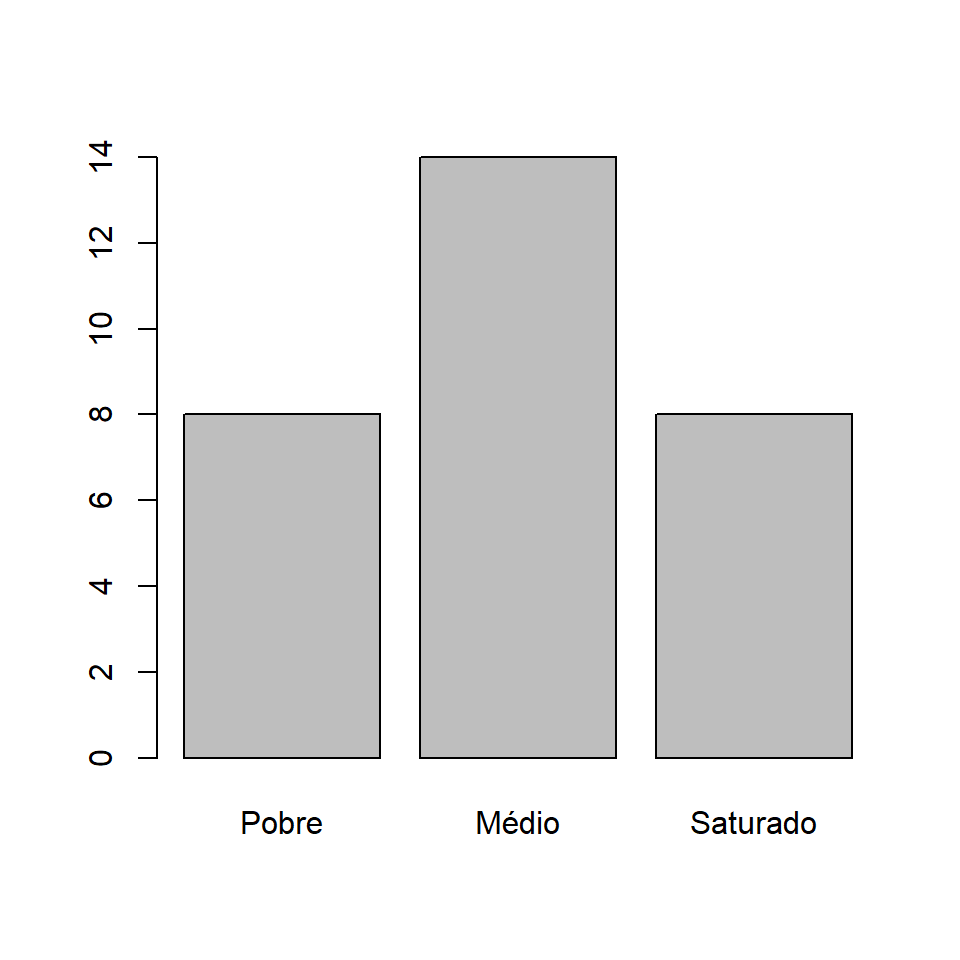
\includegraphics{IntroR_files/figure-latex/unnamed-chunk-105-1} \end{center}

Melhorando a formatação gráfica:

\begin{Shaded}
\begin{Highlighting}[]
\FunctionTok{barplot}\NormalTok{(tab1,}
        \AttributeTok{main =} \StringTok{"Concentração de oxigênio"}\NormalTok{,}
        \AttributeTok{ylab =} \StringTok{"Frequência"}\NormalTok{,}
        \AttributeTok{ylim =} \FunctionTok{c}\NormalTok{(}\DecValTok{0}\NormalTok{, }\DecValTok{18}\NormalTok{), }\AttributeTok{col =} \StringTok{"black"}\NormalTok{)}
\FunctionTok{box}\NormalTok{()}
\end{Highlighting}
\end{Shaded}

\begin{center}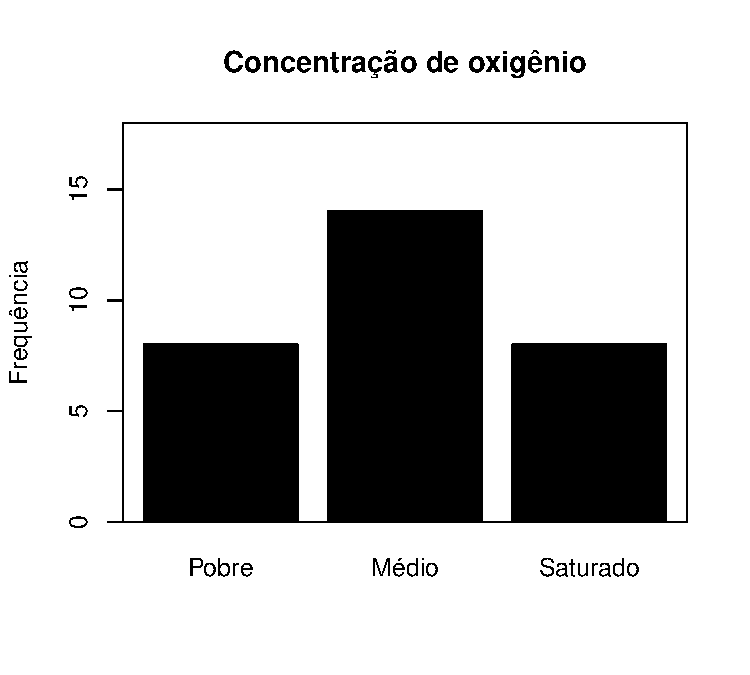
\includegraphics{IntroR_files/figure-latex/unnamed-chunk-106-1} \end{center}

\hypertarget{histograma}{%
\subsection{Histograma}\label{histograma}}

Um histograma é a forma mais direta de avaliarmos o padrão de distribuição de uma variável quantitativa. Um histograma é construído a partir da divisão de uma variável em \emph{intervalos de classe} e contando o número de classes dentro deste intervalo.

Veja o histograma abaixo para a oxy que expressa a concentração de oxigênio em mg/l \(\times\) 10.

\begin{Shaded}
\begin{Highlighting}[]
\FunctionTok{hist}\NormalTok{(ambiente}\SpecialCharTok{$}\NormalTok{oxy)}
\end{Highlighting}
\end{Shaded}

\begin{center}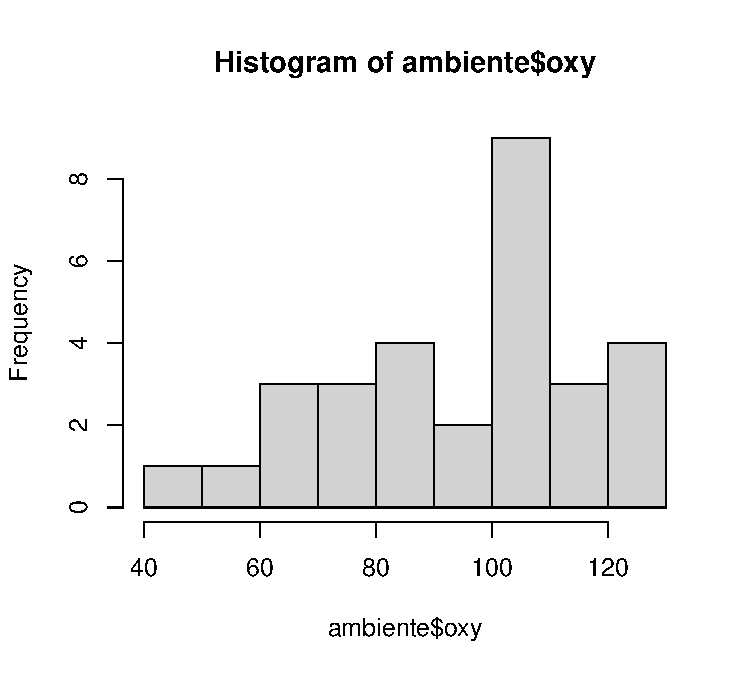
\includegraphics{IntroR_files/figure-latex/unnamed-chunk-108-1} \end{center}

A figura mostra por exemplo que existe 1 seção com concentração entre 40 e 50 mg/l \(\times\) 10, e 2 seções com concentração entre 90 e 100 mg/l \(\times\) 10. Verifique quais são estes veículos com o comando abaixo:

\begin{Shaded}
\begin{Highlighting}[]
\NormalTok{ambiente[}\FunctionTok{order}\NormalTok{(ambiente}\SpecialCharTok{$}\NormalTok{oxy),]}
\end{Highlighting}
\end{Shaded}

\begin{verbatim}
##     dfs alt   slo  flo pH har pho nit amm oxy bdo   secao   trofia
## 25 3278 231 1.792 3870 79 100 422 620 180  41 167 Seção 3    Pobre
## 24 3147 241 1.386 2976 80  99 140 250  60  52 123 Seção 3    Pobre
## 26 3579 214 1.792 3910 79  94 143 300  30  62  89 Seção 4    Pobre
## 23 3043 246 2.565 2880 81  97 260 350 115  63 164 Seção 3    Pobre
## 8   491 792 3.258  130 81  94  20  41  12  70  81 Seção 1    Pobre
## 9   705 752 2.565  480 80  90  30  82  12  72  52 Seção 2    Pobre
## 27 3732 206 2.565 3960 81  90  58 300  26  72  63 Seção 4    Pobre
## 5   215 849 3.178  264 81  84  38  52  20  80  62 Seção 2    Pobre
## 28 3947 195 1.386 4320 83 100  74 400  30  81  45 Seção 4    Médio
## 30 4530 172 1.099 6900 82 109  65 160  10  82  44 Seção 4    Médio
## 21 2812 262 2.398 2720 79  85  20 220  10  90  41 Seção 4    Médio
## 29 4220 183 1.946 6770 78 110  45 162  10  90  42 Seção 4    Médio
## 22 2940 254 2.708 2790 81  88  20 162   7  91  48 Seção 4    Médio
## 10  990 617 4.605 1000 77  82   6  75   1 100  43 Seção 1    Médio
## 6   324 846 3.497  286 79  60  20  15   0 102  53 Seção 1    Médio
## 17 1985 348 1.792 2430 80  92  20 250  20 102  46 Seção 2    Médio
## 2    22 932 3.434  100 80  40   2  20  10 103  19 Seção 1    Médio
## 16 1859 375 3.045 1610 80  88  20 200   5 103  27 Seção 1    Médio
## 18 2110 332 2.197 2500 80  90  50 220  20 103  28 Seção 4    Médio
## 20 2477 286 2.197 2680 80  86  30 300  30 103  28 Seção 4    Médio
## 3   102 914 3.638  180 83  52   5  22   5 105  35 Seção 1    Médio
## 19 2246 310 1.792 2590 81  84  60 220  15 106  33 Seção 4    Médio
## 4   185 854 3.497  253 80  72  10  21   0 110  13 Seção 1 Saturado
## 7   268 841 4.205  400 81  88   7  15   0 111  22 Seção 1 Saturado
## 11 1234 483 3.738 1990 81  96  30 160   0 115  27 Seção 1 Saturado
## 15 1645 415 1.792 2300 86  86  40 100   0 117  21 Seção 1 Saturado
## 1     3 934 6.176   84 79  45   1  20   0 122  27 Seção 1 Saturado
## 12 1324 477 2.833 2000 79  86   4  50   0 122  30 Seção 1 Saturado
## 14 1522 434 2.565 2120 83  98  27 123   0 123  38 Seção 1 Saturado
## 13 1436 450 3.091 2110 81  98   6  52   0 124  24 Seção 1 Saturado
\end{verbatim}

Em um histograma, a escolha do intervalo de classes determina o formato exato do gráfico. No exemplo acima, a escolha foi feita automaticamente. No entanto, podemos definir esplicitamente o intervalo desejado utilizando o argumento \texttt{breaks} conforme abaixo:

\begin{Shaded}
\begin{Highlighting}[]
\NormalTok{classes }\OtherTok{\textless{}{-}} \FunctionTok{seq}\NormalTok{(}\DecValTok{40}\NormalTok{, }\DecValTok{140}\NormalTok{, }\AttributeTok{by =} \DecValTok{20}\NormalTok{)}
\FunctionTok{hist}\NormalTok{(ambiente}\SpecialCharTok{$}\NormalTok{oxy, }\AttributeTok{breaks =}\NormalTok{ classes)}
\end{Highlighting}
\end{Shaded}

\begin{center}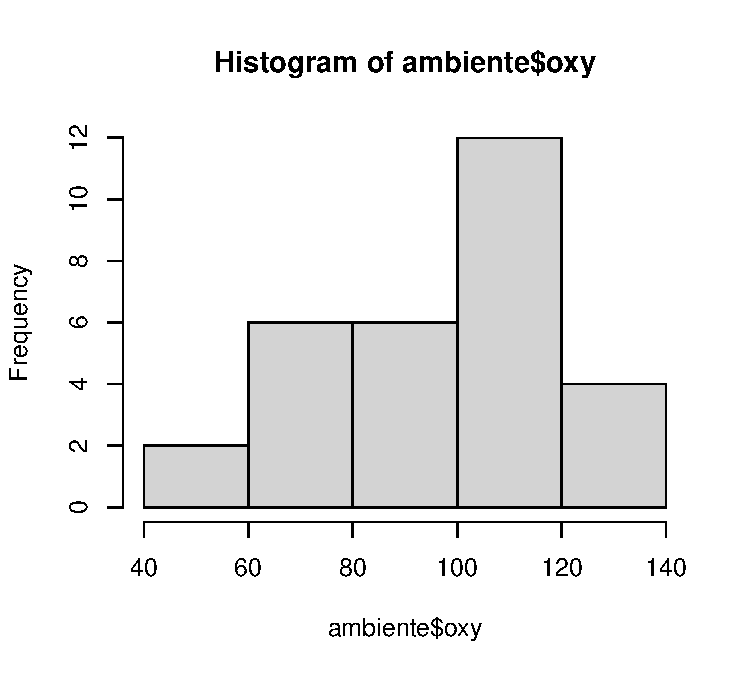
\includegraphics{IntroR_files/figure-latex/unnamed-chunk-110-1} \end{center}

Aqui fizemos a divisão em intervalos de tamanho 20, iniciando em 40 e terminando em 140. A escolha do tamanho das classes é de certa forma arbitrária e definida para que o figura evidencie da melhor forma possível o padrão de distribuição dos dados.

\hypertarget{boxplot}{%
\subsection{Boxplot}\label{boxplot}}

Boxplots oferecem um \emph{resumo gráfico} da distribuição de uma variável quantitativa. Abaixo veja um boxplot da variável oxy.

\begin{Shaded}
\begin{Highlighting}[]
\FunctionTok{boxplot}\NormalTok{(ambiente}\SpecialCharTok{$}\NormalTok{oxy)}
\end{Highlighting}
\end{Shaded}

\begin{center}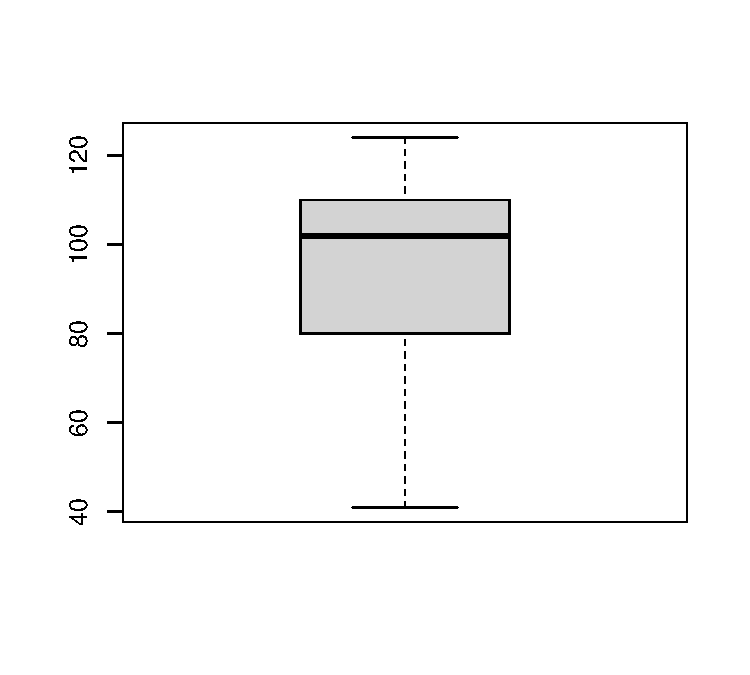
\includegraphics{IntroR_files/figure-latex/unnamed-chunk-111-1} \end{center}

No boxplot, a linha do meio representa a \textbf{mediana} dos dados, os limitres das caixas representam o \(1^o\) e \(3^o\) percentis e as linhas os pontos mínimo e máximo. Podemos ver quais são estes valores com o comando:

\begin{Shaded}
\begin{Highlighting}[]
\FunctionTok{quantile}\NormalTok{(ambiente}\SpecialCharTok{$}\NormalTok{oxy, }\AttributeTok{probs =} \FunctionTok{c}\NormalTok{(}\DecValTok{0}\NormalTok{, }\FloatTok{0.25}\NormalTok{, }\FloatTok{0.5}\NormalTok{, }\FloatTok{0.75}\NormalTok{, }\DecValTok{1}\NormalTok{))}
\end{Highlighting}
\end{Shaded}

\begin{verbatim}
##     0%    25%    50%    75%   100% 
##  41.00  80.25 102.00 109.00 124.00
\end{verbatim}

\hypertarget{visualizando-associauxe7uxf5es-entre-duas-variuxe1veis}{%
\section{Visualizando associações entre duas variáveis}\label{visualizando-associauxe7uxf5es-entre-duas-variuxe1veis}}

\hypertarget{gruxe1fico-de-barras-1}{%
\subsection{Gráfico de barras}\label{gruxe1fico-de-barras-1}}

Passando aos gráficos bi-variados, vamos criar um gráfico de barras combinando as variáveis categóricas \texttt{secao} e \texttt{trofia}. Como fizemos anteriormente, montamos uma tabela de frequência, porpém neste caso combinando as duas variáveis.

\begin{Shaded}
\begin{Highlighting}[]
\NormalTok{tab2 }\OtherTok{\textless{}{-}} \FunctionTok{table}\NormalTok{(ambiente[,}\FunctionTok{c}\NormalTok{(}\StringTok{"secao"}\NormalTok{, }\StringTok{"trofia"}\NormalTok{)])}
\NormalTok{tab2}
\end{Highlighting}
\end{Shaded}

\begin{verbatim}
##          trofia
## secao     Pobre Médio Saturado
##   Seção 1     1     5        8
##   Seção 2     2     1        0
##   Seção 3     3     0        0
##   Seção 4     2     8        0
\end{verbatim}

Neste caso, podemos fazer gráficos de barras de quatro formas distintas:

\begin{Shaded}
\begin{Highlighting}[]
\FunctionTok{layout}\NormalTok{(}\AttributeTok{mat =} \FunctionTok{matrix}\NormalTok{(}\DecValTok{1}\SpecialCharTok{:}\DecValTok{4}\NormalTok{, }\AttributeTok{nrow =} \DecValTok{2}\NormalTok{, }\AttributeTok{ncol =} \DecValTok{2}\NormalTok{, }\AttributeTok{byrow =} \ConstantTok{TRUE}\NormalTok{))}
\FunctionTok{barplot}\NormalTok{(tab2, }\AttributeTok{legend =} \ConstantTok{TRUE}\NormalTok{)}
\FunctionTok{barplot}\NormalTok{(tab2, }\AttributeTok{legend =} \ConstantTok{TRUE}\NormalTok{, }\AttributeTok{beside =} \ConstantTok{TRUE}\NormalTok{)}
\FunctionTok{barplot}\NormalTok{(}\FunctionTok{t}\NormalTok{(tab2), }\AttributeTok{legend =} \ConstantTok{TRUE}\NormalTok{)}
\FunctionTok{barplot}\NormalTok{(}\FunctionTok{t}\NormalTok{(tab2), }\AttributeTok{legend =} \ConstantTok{TRUE}\NormalTok{, }\AttributeTok{beside =} \ConstantTok{TRUE}\NormalTok{)}
\end{Highlighting}
\end{Shaded}

\begin{center}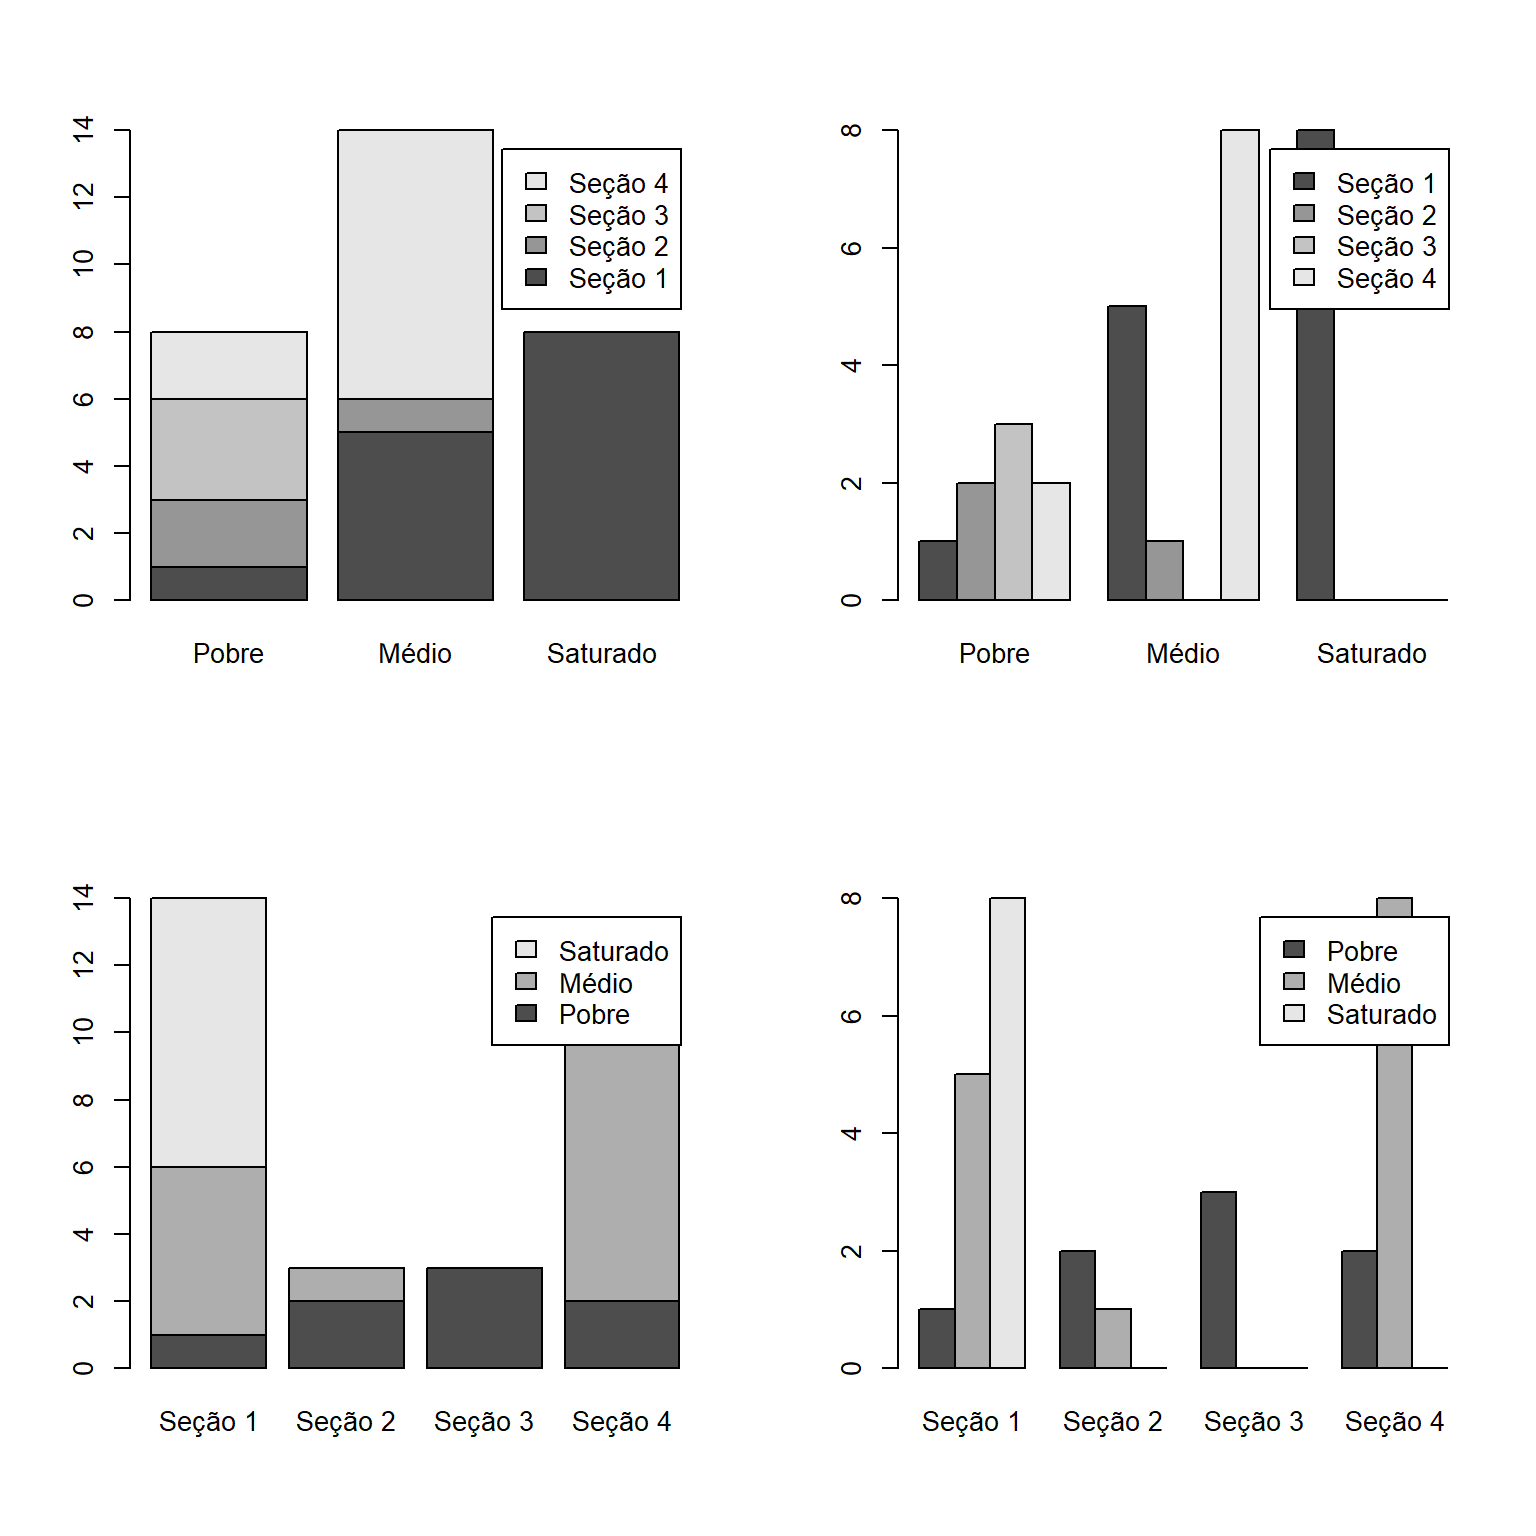
\includegraphics{IntroR_files/figure-latex/unnamed-chunk-114-1} \end{center}

O comando acima necessita de algumas esplicações.

\begin{enumerate}
\def\labelenumi{\arabic{enumi}.}
\item
  A função \texttt{layout(mat\ =\ matrix(1:4,\ nrow\ =\ 2,\ ncol\ =\ 2,\ byrow\ =\ TRUE))} organiza o espaço gráfico em um formato matricial com 2 linhas por 2 colunas, permitindo a inserrção de 4 figuras. O argumento \texttt{byrow\ =\ TRUE} define que as figuras serão adicionais linha-a-linha;
\item
  A expressão \texttt{t(tab2)} tem como resultado \emph{tanspor} a tabela, o que consequentemente altera a referência da figura. No primeiro caso, a referência é a concentração de oxigêncio e no segundo caso, as seções;
\item
  O argumento \texttt{beside\ =\ TRUE} faz com que todas as barras apareçam lado-a-lado. Caso contrário, cada barra representa uma coluna da matriz \texttt{tab2} ou da sua transposta \texttt{t(tab2)};
\item
  Em todos os gráficos foi adicionada uma legenda para permitir a interpretação dos gráficos;
\end{enumerate}

Aqui vale melhorarmos a formatação:

\begin{Shaded}
\begin{Highlighting}[]
\NormalTok{cores }\OtherTok{\textless{}{-}} \DecValTok{1}\SpecialCharTok{:}\DecValTok{4}
\NormalTok{limy1 }\OtherTok{\textless{}{-}} \FunctionTok{c}\NormalTok{(}\DecValTok{0}\NormalTok{, }\DecValTok{17}\NormalTok{)}
\NormalTok{limy2 }\OtherTok{\textless{}{-}} \FunctionTok{c}\NormalTok{(}\DecValTok{0}\NormalTok{, }\DecValTok{16}\NormalTok{)}
\NormalTok{legenda }\OtherTok{\textless{}{-}} \FunctionTok{list}\NormalTok{(}\AttributeTok{cex =} \FloatTok{0.8}\NormalTok{)}

\FunctionTok{layout}\NormalTok{(}\AttributeTok{mat =} \FunctionTok{matrix}\NormalTok{(}\DecValTok{1}\SpecialCharTok{:}\DecValTok{4}\NormalTok{, }\AttributeTok{nrow =} \DecValTok{2}\NormalTok{, }\AttributeTok{ncol =} \DecValTok{2}\NormalTok{, }\AttributeTok{byrow =} \ConstantTok{TRUE}\NormalTok{))}
\FunctionTok{barplot}\NormalTok{(tab2, }\AttributeTok{legend =} \ConstantTok{TRUE}\NormalTok{, }\AttributeTok{col =}\NormalTok{ cores, }\AttributeTok{ylim =}\NormalTok{ limy1, }
        \AttributeTok{args.legend =}\NormalTok{ legenda)}
\FunctionTok{box}\NormalTok{()}
\FunctionTok{barplot}\NormalTok{(tab2, }\AttributeTok{legend =} \ConstantTok{TRUE}\NormalTok{, }\AttributeTok{beside =} \ConstantTok{TRUE}\NormalTok{, }\AttributeTok{col =}\NormalTok{ cores, }
        \AttributeTok{ylim =}\NormalTok{ limy1, }\AttributeTok{args.legend =}\NormalTok{ legenda)}
\FunctionTok{box}\NormalTok{()}
\FunctionTok{barplot}\NormalTok{(}\FunctionTok{t}\NormalTok{(tab2), }\AttributeTok{legend =} \ConstantTok{TRUE}\NormalTok{, }\AttributeTok{col =}\NormalTok{ cores, }\AttributeTok{ylim =}\NormalTok{ limy2, }
        \AttributeTok{args.legend =}\NormalTok{ legenda)}
\FunctionTok{box}\NormalTok{()}
\FunctionTok{barplot}\NormalTok{(}\FunctionTok{t}\NormalTok{(tab2), }\AttributeTok{legend =} \ConstantTok{TRUE}\NormalTok{, }\AttributeTok{beside =} \ConstantTok{TRUE}\NormalTok{, }\AttributeTok{col =}\NormalTok{ cores, }
        \AttributeTok{ylim =}\NormalTok{ limy2, }\AttributeTok{args.legend =}\NormalTok{ legenda)}
\FunctionTok{box}\NormalTok{()}
\end{Highlighting}
\end{Shaded}

\begin{center}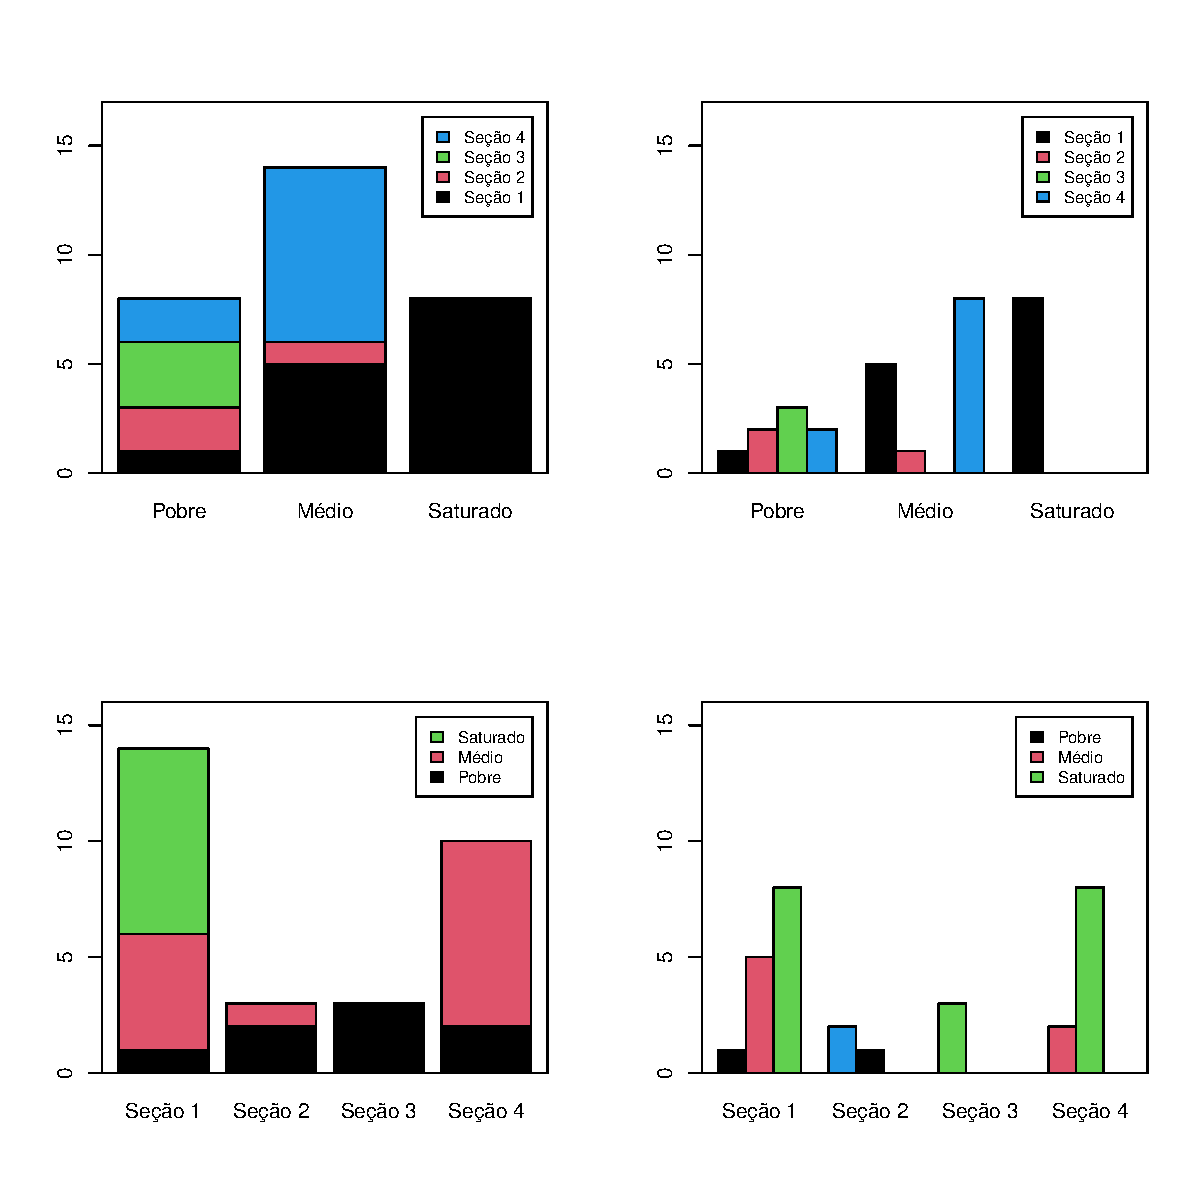
\includegraphics{IntroR_files/figure-latex/unnamed-chunk-115-1} \end{center}

\hypertarget{boxplot-1}{%
\subsection{Boxplot}\label{boxplot-1}}

O boxplot é mais utilizado na situação a seguir em que queremos sumarizar uma variável quantitativa para diferentes níveis de uma variável categórica. Para isto, vamos associar a variável oxy à variável secao.

\begin{Shaded}
\begin{Highlighting}[]
\FunctionTok{boxplot}\NormalTok{(oxy }\SpecialCharTok{\textasciitilde{}}\NormalTok{ secao, }\AttributeTok{data =}\NormalTok{ ambiente)}
\end{Highlighting}
\end{Shaded}

\begin{center}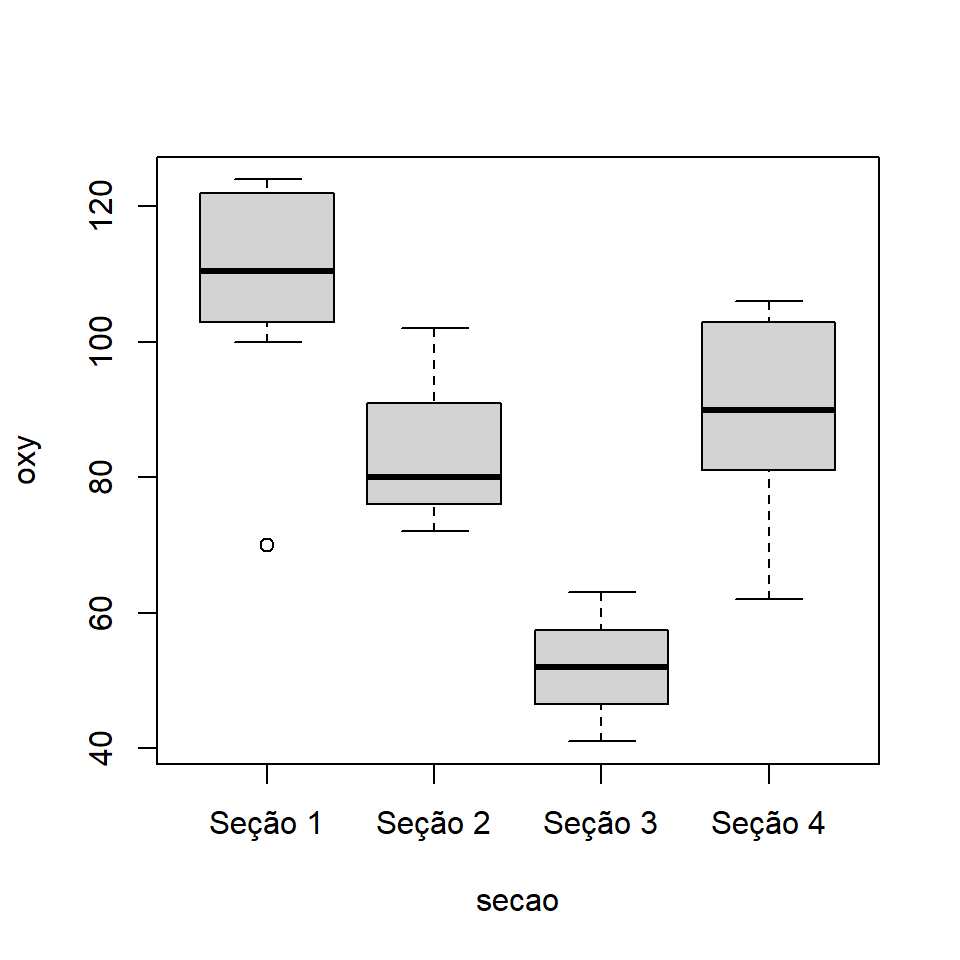
\includegraphics{IntroR_files/figure-latex/unnamed-chunk-116-1} \end{center}

Vemos que \emph{aparentemente} os pontos associados ao \texttt{Seção\ 1} têm maiores concentrações de oxigênio (mediana = NA) e que os pontos associados à \texttt{Seção\ 3} os menores valores (mediana = 52). É neste tipo de comparação que geralmente estamos interessados ao fazer um boxplot deste tipo.

Aqui utilizamos uma notação diferente.

\begin{enumerate}
\def\labelenumi{\arabic{enumi}.}
\item
  Ao invés de dizermos explicitamente qual variável está no eixo \texttt{y} e qual está no eixo \texttt{x}, utilizamos o símbolo \texttt{\textasciitilde{}} para expressar que \texttt{y} \emph{depende de} \texttt{x}. Esta notação é amplamente utilizada em modelos estatísticos como Regressão e Análise de Variância e está associada aos conceitos de variável \emph{dependente} (ou \emph{reposta}, \texttt{y}) e de variável \emph{independente} (ou \emph{preditora}, \texttt{x}). Neste caso, então a concentração de oxigênio \emph{depende} da seção do rio.
\item
  Ao invés de chamarmos a variável por \texttt{ambiente\$oxy}, utilizamos somente o nome da coluna (\texttt{oxy}) e adicionamos o argumento \texttt{data\ =\ ambiente} para indicar em qual data frame a função irá buscar as variáveis. Deste ponto em diante iremos utilizar esta notação sempre que possível, para que você se familiarize com sua utilização na prática de ajuste de modelos estatísticos no R.
\end{enumerate}

\hypertarget{gruxe1fico-de-dispersuxe3o}{%
\subsection{Gráfico de dispersão}\label{gruxe1fico-de-dispersuxe3o}}

Um gráfico de dispersão mostra a associação entre duas variáveis quantitativas. Vamos verificar a associação entre concentração de nitrato (mg/l \(\times\) 100) e a distância da foz (km \(\times\) 10). Neste caso, é fundamental definirmos quem serão as variáveis dependentes e independentes. Aqui, faz sentido pensar que a concentração de nitrato varia \textbf{em função} da distância da foz e não o contrário.

\begin{Shaded}
\begin{Highlighting}[]
\FunctionTok{plot}\NormalTok{(nit }\SpecialCharTok{\textasciitilde{}}\NormalTok{ dfs, }\AttributeTok{data =}\NormalTok{ ambiente)}
\end{Highlighting}
\end{Shaded}

\begin{center}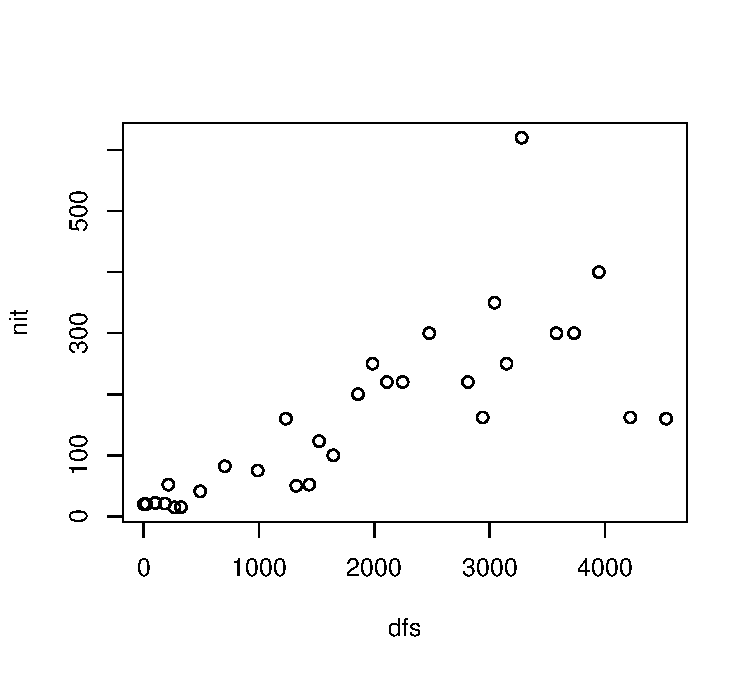
\includegraphics{IntroR_files/figure-latex/unnamed-chunk-117-1} \end{center}

Os resultados aqui parecem expressar uma relação esperada em que a concentração de nutrientes aumenta à medida que nos aproximamos da foz de rio e riachos.

Novamente, vamos aproveitar para falar um pouco sobre formatação gráfica alterando os nomes dos eixos(argumentos \texttt{xlab} e \texttt{ylab}), tipo de ponto (argumento \texttt{pch}).

\begin{Shaded}
\begin{Highlighting}[]
\FunctionTok{plot}\NormalTok{(nit }\SpecialCharTok{\textasciitilde{}}\NormalTok{ dfs, }\AttributeTok{data =}\NormalTok{ ambiente,}
     \AttributeTok{xlab =} \FunctionTok{bquote}\NormalTok{(}\StringTok{"Vazão média mínima (m"} \SpecialCharTok{\^{}}\DecValTok{3}\SpecialCharTok{/}\StringTok{"seg x 100)"}\NormalTok{),}
     \AttributeTok{ylab =} \FunctionTok{bquote}\NormalTok{(}\StringTok{"Concentração de Nitrato (mg"}\SpecialCharTok{/}\StringTok{"l x 100)"}\NormalTok{),}
     \AttributeTok{pch =} \DecValTok{19}
\NormalTok{)}
\end{Highlighting}
\end{Shaded}

\begin{center}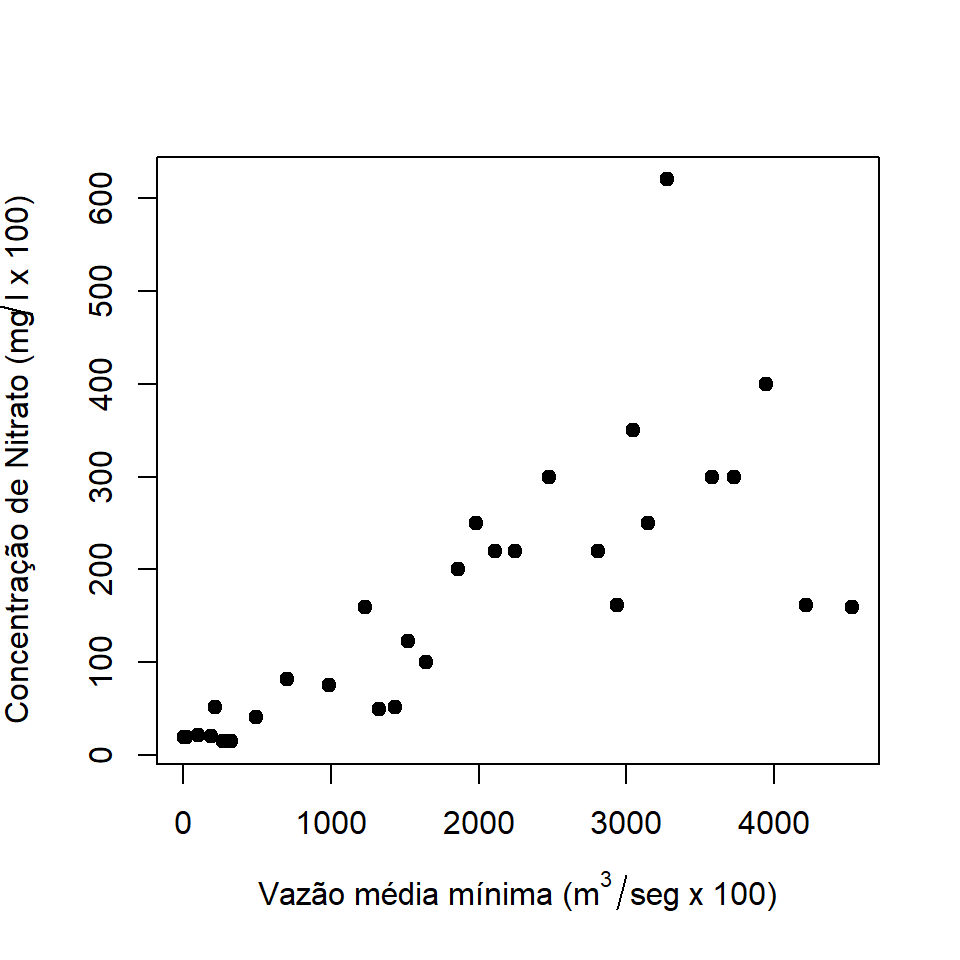
\includegraphics{IntroR_files/figure-latex/unnamed-chunk-118-1} \end{center}

\hypertarget{compreendendo-o-ambiente-por-meio-de-suas-variuxe1veis}{%
\section{Compreendendo o ambiente por meio de suas variáveis}\label{compreendendo-o-ambiente-por-meio-de-suas-variuxe1veis}}

Em um estudo como o de Verneaux \citep{Verneaux1973} o objetivo e entender os sistema de riachos por meio das variáveis que escolhemos quantificar e como o modo como escolermos visualizá-las. Os gráficos vistos acima não são certamente a única forma de imcorporar variáveis em uma figura. As possibilidade de manipulação de cores, símbolos e textos no ambiente gráfico fornece formas adicionais de incluirmos uma determinada informação. Nesta seção vamos explorar um pouco melhor estas questões.

Dissemos que os pontos de amostragem foram obtidos ao longo do gradiente cabeceira-foz de um rio na França. Parte das informações que temos se referem às coordenadas geográficas destes pontos (no data frame \texttt{\$yx}). Verifique também que a sequência dos pontos segue uma ordem crescente da distância da foz. Inicialmente, vamos plotar as coordenadas geográficas de todos os pontos utilizando um gráfico de linhas:

\begin{Shaded}
\begin{Highlighting}[]
\FunctionTok{plot}\NormalTok{(}\AttributeTok{x =}\NormalTok{ doubs}\SpecialCharTok{$}\NormalTok{xy}\SpecialCharTok{$}\NormalTok{x, }\AttributeTok{y =}\NormalTok{ doubs}\SpecialCharTok{$}\NormalTok{xy}\SpecialCharTok{$}\NormalTok{y, }\AttributeTok{type =} \StringTok{"l"}\NormalTok{,}
     \AttributeTok{xlab =} \StringTok{"Coordenada em x (km)"}\NormalTok{, }
     \AttributeTok{ylab =} \StringTok{"Coordenada em y (km)"}\NormalTok{,}
     \AttributeTok{col =} \StringTok{"\#4287f5"}\NormalTok{, }\AttributeTok{lwd =} \DecValTok{3}\NormalTok{)}
\end{Highlighting}
\end{Shaded}

\begin{center}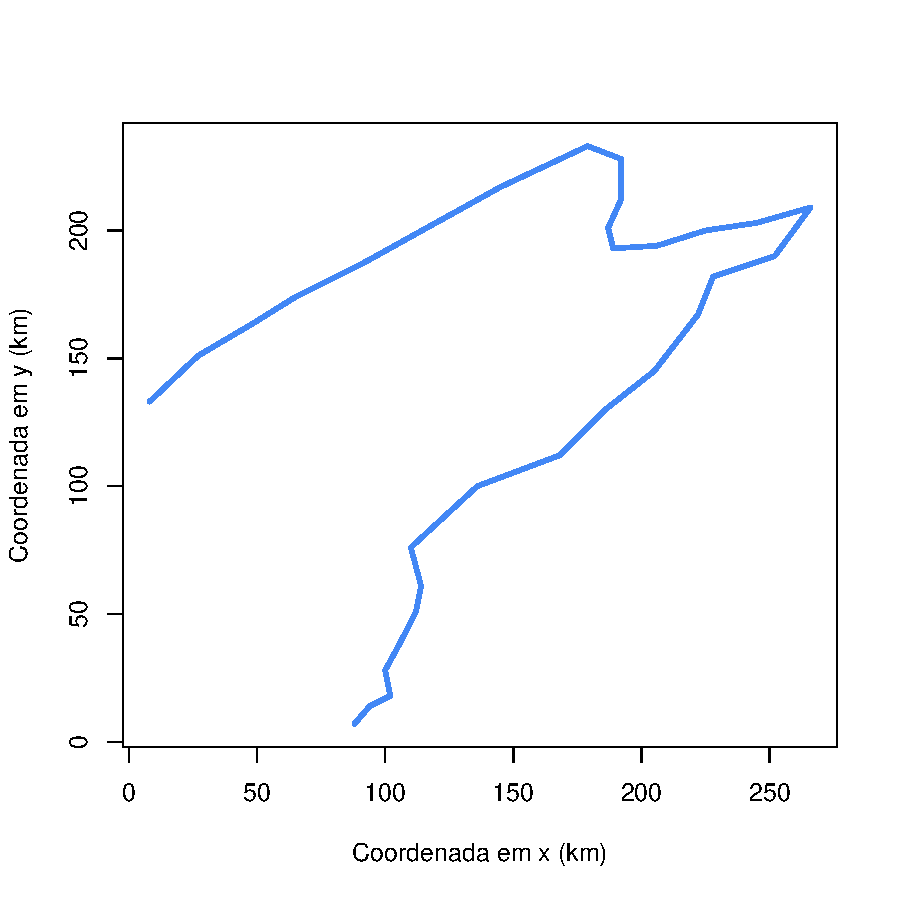
\includegraphics{IntroR_files/figure-latex/unnamed-chunk-119-1} \end{center}

Compare, a figura com o desenho do \href{https://pt.wikipedia.org/wiki/Rio_Doubs}{rio Doubs}.

\begin{itemize}
\tightlist
\item
  obs: utilizamos aqui a definição de cores em \textbf{HEXADECIMAL}. Você pode fazer o mesmo, escolhendo a cor desejada aqui: \href{https://www.google.com/search?q=hex+color+picker\&oq=hex+color+picker\&aqs=chrome..69i57j0l7.11304j0j4\&sourceid=chrome\&ie=UTF-8}{hex color picker}.
\end{itemize}

Vamos indicar os pontos de cabeceira e foz.

\begin{Shaded}
\begin{Highlighting}[]
\NormalTok{pontos\_extremos }\OtherTok{\textless{}{-}}\NormalTok{ doubs}\SpecialCharTok{$}\NormalTok{xy[}\FunctionTok{which}\NormalTok{(doubs}\SpecialCharTok{$}\NormalTok{env}\SpecialCharTok{$}\NormalTok{dfs }\SpecialCharTok{==} \FunctionTok{min}\NormalTok{(doubs}\SpecialCharTok{$}\NormalTok{env}\SpecialCharTok{$}\NormalTok{dfs) }\SpecialCharTok{|} 
\NormalTok{                                      doubs}\SpecialCharTok{$}\NormalTok{env}\SpecialCharTok{$}\NormalTok{dfs }\SpecialCharTok{==} \FunctionTok{max}\NormalTok{(doubs}\SpecialCharTok{$}\NormalTok{env}\SpecialCharTok{$}\NormalTok{dfs)),]}
\FunctionTok{plot}\NormalTok{(}\AttributeTok{x =}\NormalTok{ doubs}\SpecialCharTok{$}\NormalTok{xy}\SpecialCharTok{$}\NormalTok{x, }\AttributeTok{y =}\NormalTok{ doubs}\SpecialCharTok{$}\NormalTok{xy}\SpecialCharTok{$}\NormalTok{y, }\AttributeTok{type =} \StringTok{"l"}\NormalTok{,}
     \AttributeTok{xlab =} \StringTok{"Coordenada em x (km)"}\NormalTok{, }
     \AttributeTok{ylab =} \StringTok{"Coordenada em y (km)"}\NormalTok{,}
     \AttributeTok{col =} \StringTok{"\#4287f5"}\NormalTok{, }\AttributeTok{lwd =} \DecValTok{3}\NormalTok{)}
\FunctionTok{text}\NormalTok{(}\AttributeTok{x =}\NormalTok{ pontos\_extremos}\SpecialCharTok{$}\NormalTok{x, }
       \AttributeTok{y =}\NormalTok{ pontos\_extremos}\SpecialCharTok{$}\NormalTok{y,}
       \AttributeTok{labels =} \FunctionTok{c}\NormalTok{(}\StringTok{"Cabeceira"}\NormalTok{, }\StringTok{"Foz"}\NormalTok{))}
\end{Highlighting}
\end{Shaded}

\begin{center}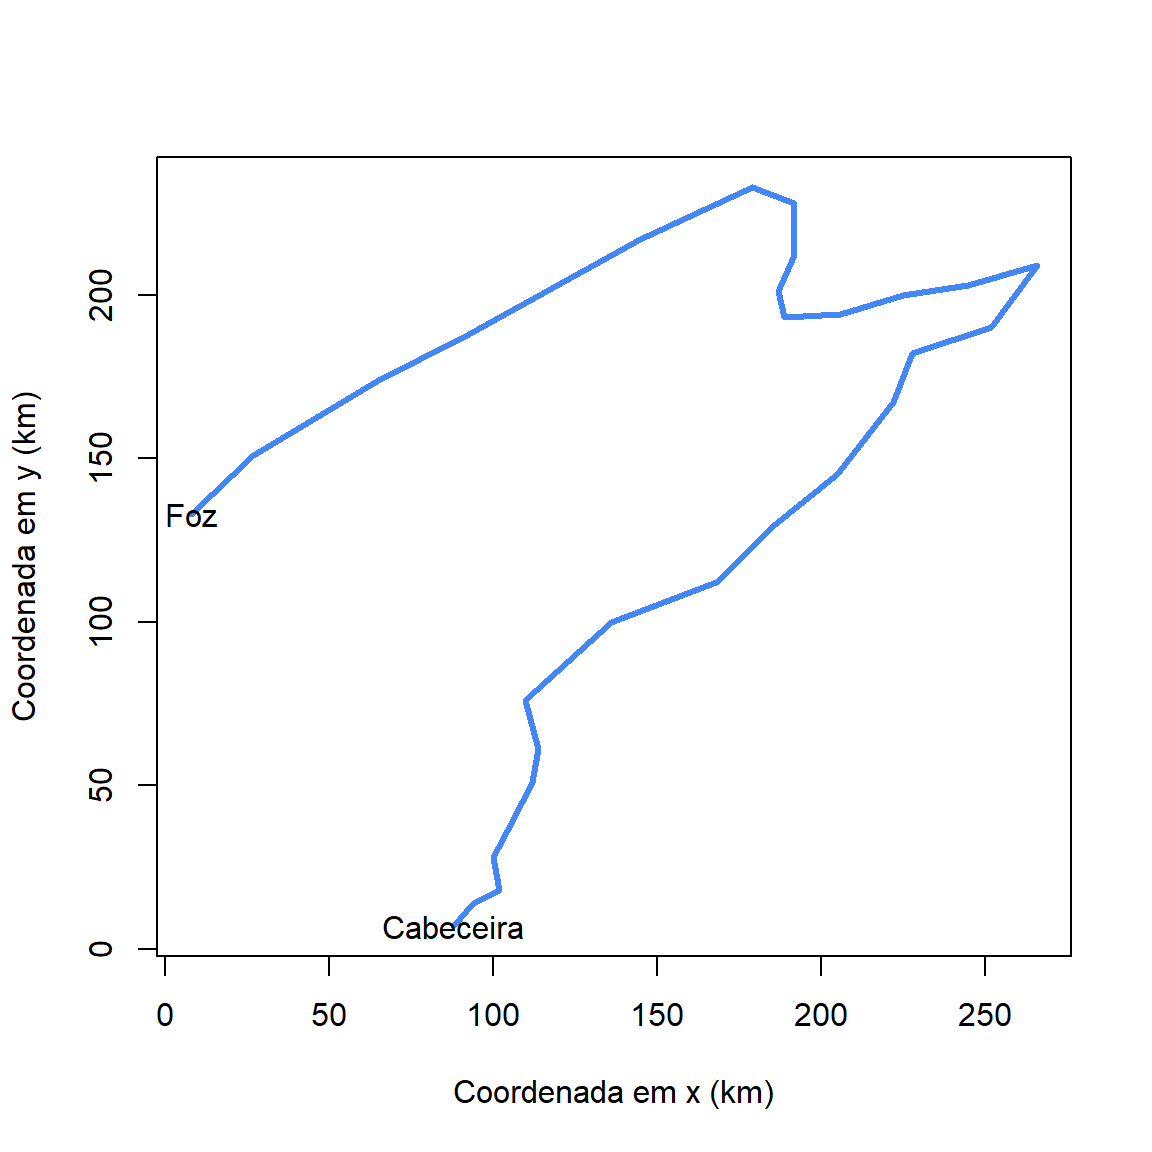
\includegraphics{IntroR_files/figure-latex/unnamed-chunk-120-1} \end{center}

Lembre-se que definimos acima 4 trechos. Vamos ver onde estes seções se localizam plotando-os com cores distintas.

\begin{Shaded}
\begin{Highlighting}[]
\NormalTok{secao\_cor }\OtherTok{\textless{}{-}} \FunctionTok{as.numeric}\NormalTok{(ambiente}\SpecialCharTok{$}\NormalTok{secao)}

\FunctionTok{plot}\NormalTok{(}\AttributeTok{x =}\NormalTok{ doubs}\SpecialCharTok{$}\NormalTok{xy}\SpecialCharTok{$}\NormalTok{x, }\AttributeTok{y =}\NormalTok{ doubs}\SpecialCharTok{$}\NormalTok{xy}\SpecialCharTok{$}\NormalTok{y, }\AttributeTok{type =} \StringTok{"l"}\NormalTok{,}
     \AttributeTok{xlab =} \StringTok{"Coordenada em x (km)"}\NormalTok{, }
     \AttributeTok{ylab =} \StringTok{"Coordenada em y (km)"}\NormalTok{,}
     \AttributeTok{col =} \StringTok{"\#4287f5"}\NormalTok{, }\AttributeTok{lwd =} \DecValTok{3}\NormalTok{)}
\FunctionTok{points}\NormalTok{(}\AttributeTok{x =}\NormalTok{ doubs}\SpecialCharTok{$}\NormalTok{xy}\SpecialCharTok{$}\NormalTok{x, }\AttributeTok{y =}\NormalTok{ doubs}\SpecialCharTok{$}\NormalTok{xy}\SpecialCharTok{$}\NormalTok{y, }\AttributeTok{pch =} \DecValTok{21}\NormalTok{, }
       \AttributeTok{bg =}\NormalTok{ secao\_cor, }\AttributeTok{cex =} \DecValTok{3}\NormalTok{)}
\FunctionTok{legend}\NormalTok{(}\AttributeTok{x =} \StringTok{"bottomright"}\NormalTok{, }\AttributeTok{col =} \DecValTok{1}\SpecialCharTok{:}\DecValTok{4}\NormalTok{, }
       \AttributeTok{legend =} \FunctionTok{levels}\NormalTok{(ambiente}\SpecialCharTok{$}\NormalTok{secao), }\AttributeTok{bty =} \StringTok{"n"}\NormalTok{, }\AttributeTok{pch =} \DecValTok{19}\NormalTok{)}
\end{Highlighting}
\end{Shaded}

\begin{center}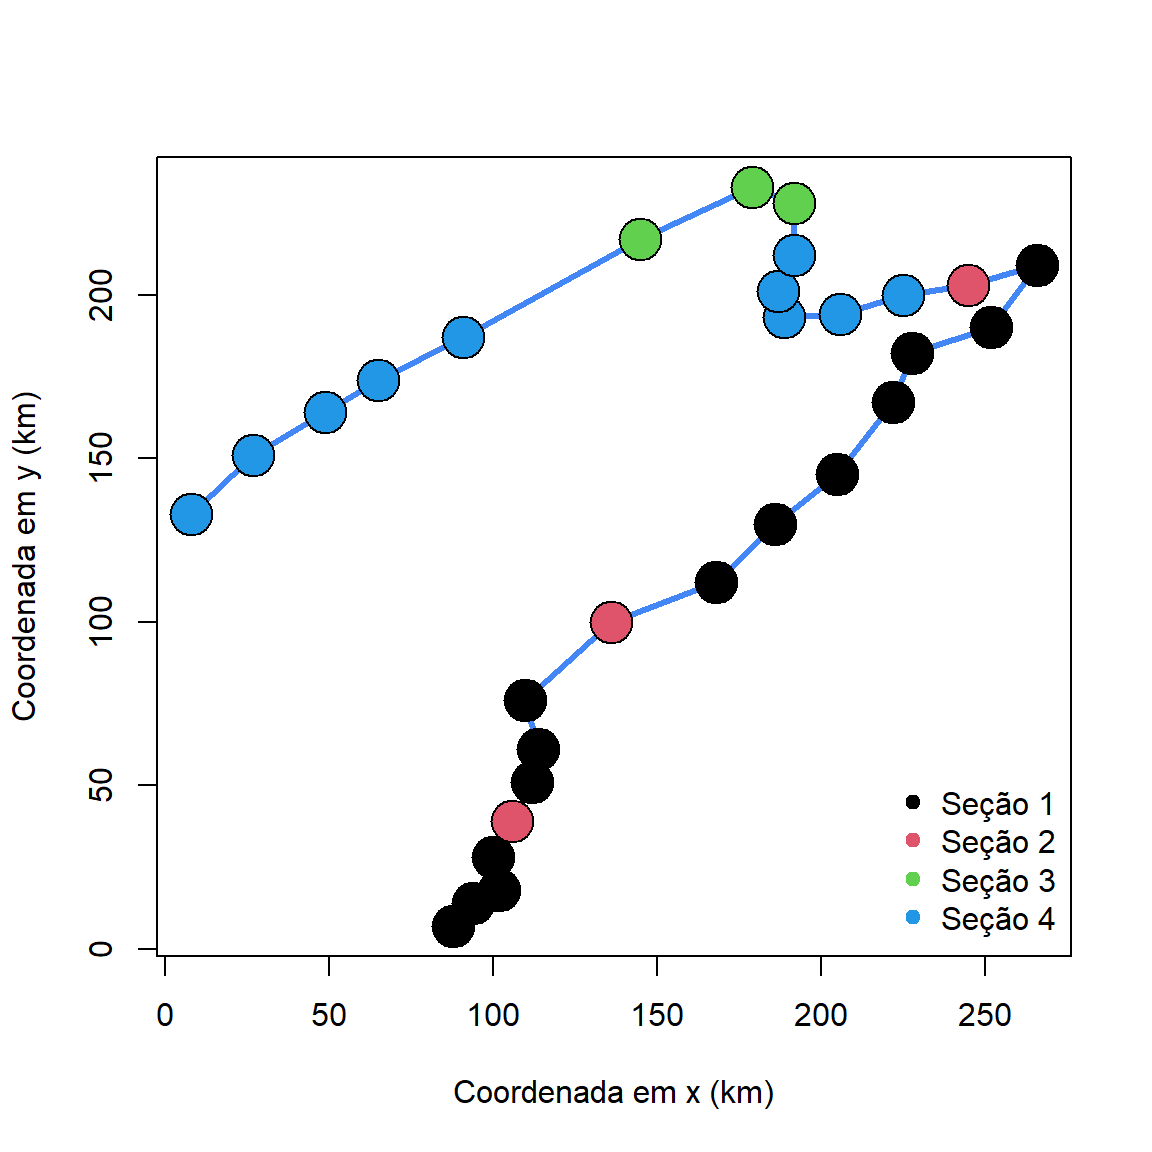
\includegraphics{IntroR_files/figure-latex/unnamed-chunk-121-1} \end{center}

Aqui fica clara a divisão principal entre os grupos referente às seções 1 e 2 na metade superior do rio e as seções 3 e 4 na metade inferior. Para continuar explorando os dados, vamos inserir a informação sobre a concentração de amônia (\texttt{amm}).

\begin{Shaded}
\begin{Highlighting}[]
\NormalTok{secao\_cor }\OtherTok{\textless{}{-}} \FunctionTok{as.numeric}\NormalTok{(ambiente}\SpecialCharTok{$}\NormalTok{secao) }\SpecialCharTok{+} \DecValTok{1}

\FunctionTok{plot}\NormalTok{(}\AttributeTok{x =}\NormalTok{ doubs}\SpecialCharTok{$}\NormalTok{xy}\SpecialCharTok{$}\NormalTok{x, }\AttributeTok{y =}\NormalTok{ doubs}\SpecialCharTok{$}\NormalTok{xy}\SpecialCharTok{$}\NormalTok{y, }\AttributeTok{type =} \StringTok{"l"}\NormalTok{,}
     \AttributeTok{xlab =} \StringTok{"Coordenada em x (km)"}\NormalTok{, }
     \AttributeTok{ylab =} \StringTok{"Coordenada em y (km)"}\NormalTok{,}
     \AttributeTok{col =} \StringTok{"\#4287f5"}\NormalTok{, }\AttributeTok{lwd =} \DecValTok{3}\NormalTok{)}
\FunctionTok{points}\NormalTok{(}\AttributeTok{x =}\NormalTok{ doubs}\SpecialCharTok{$}\NormalTok{xy}\SpecialCharTok{$}\NormalTok{x, }\AttributeTok{y =}\NormalTok{ doubs}\SpecialCharTok{$}\NormalTok{xy}\SpecialCharTok{$}\NormalTok{y, }\AttributeTok{pch =} \DecValTok{21}\NormalTok{, }
       \AttributeTok{bg =}\NormalTok{ secao\_cor, }\AttributeTok{cex =} \DecValTok{4}\NormalTok{)}
\FunctionTok{legend}\NormalTok{(}\AttributeTok{x =} \StringTok{"bottomright"}\NormalTok{, }\AttributeTok{col =} \DecValTok{1}\SpecialCharTok{:}\DecValTok{4}\NormalTok{, }
       \AttributeTok{legend =} \FunctionTok{levels}\NormalTok{(ambiente}\SpecialCharTok{$}\NormalTok{secao), }\AttributeTok{bty =} \StringTok{"n"}\NormalTok{, }\AttributeTok{pch =} \DecValTok{19}\NormalTok{)}
\FunctionTok{text}\NormalTok{(}\AttributeTok{x =}\NormalTok{ doubs}\SpecialCharTok{$}\NormalTok{xy}\SpecialCharTok{$}\NormalTok{x, }\AttributeTok{y =}\NormalTok{ doubs}\SpecialCharTok{$}\NormalTok{xy}\SpecialCharTok{$}\NormalTok{y, }\AttributeTok{labels =}\NormalTok{ doubs}\SpecialCharTok{$}\NormalTok{env}\SpecialCharTok{$}\NormalTok{amm, }
     \AttributeTok{cex =} \FloatTok{0.8}\NormalTok{, }\AttributeTok{font =} \DecValTok{2}\NormalTok{)}
\FunctionTok{text}\NormalTok{(}\AttributeTok{x =} \DecValTok{55}\NormalTok{, }\AttributeTok{y =} \DecValTok{220}\NormalTok{, }\AttributeTok{labels =} \StringTok{"Concentração de amônia"}\NormalTok{)}
\FunctionTok{text}\NormalTok{(}\AttributeTok{x =} \DecValTok{25}\NormalTok{, }\AttributeTok{y =} \DecValTok{120}\NormalTok{, }\AttributeTok{label =} \StringTok{"Foz"}\NormalTok{)}
\FunctionTok{text}\NormalTok{(}\AttributeTok{x =} \DecValTok{60}\NormalTok{, }\AttributeTok{y =} \DecValTok{20}\NormalTok{, }\AttributeTok{label =} \StringTok{"Cabeceira"}\NormalTok{)}
\end{Highlighting}
\end{Shaded}

\begin{center}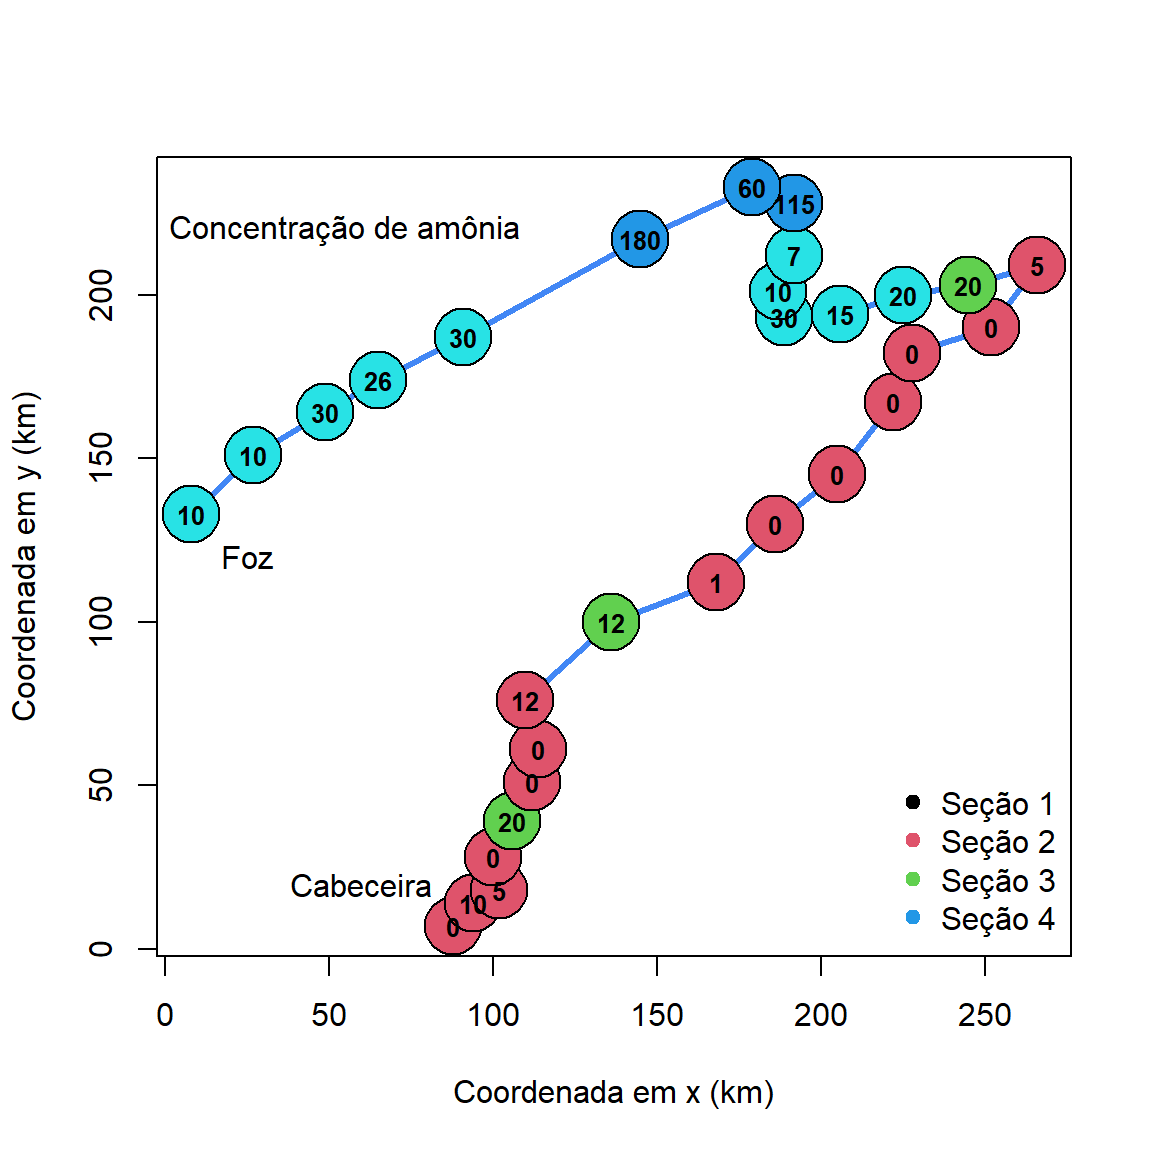
\includegraphics{IntroR_files/figure-latex/unnamed-chunk-122-1} \end{center}

Veja, que a concentração de amônia nos pontos em azul (Seção 4) é muito superior à dos pontos ao redor. Algo similar ocorre nos pontos em verde.

Provavelmente, a concentração de amônia não é a única variável pela formação destes grupos. Você pode explorar as demais variáveis químicas para verificar se outras também apresentam padrões similares.

O ponto importante e que merece ser ressaltado, é que o gráfico acima, não se enquadra em nenhuma das categorias anteriores (uni-variados, bi-variados, gráficos de barras, boxplots, etc.). No entanto, a figura nos informa sobre três variáveis: as coordenadas geográficas, a variável categórica \texttt{secao} e a concentração de amônia.

\begin{itemize}
\tightlist
\item
  Obs: utilizamos uma série de funções novas: \texttt{text}, \texttt{points}, \texttt{legend}. Para entender como elas funcionam, rode os comandos acima \textbf{linha por linha} e veja como cada função adiciona uma informação adicional à figura.
\end{itemize}

\hypertarget{mais-um-comentuxe1rio-sobre-formatauxe7uxe3o-gruxe1fica-no-r}{%
\section{Mais um comentário sobre formatação gráfica no R}\label{mais-um-comentuxe1rio-sobre-formatauxe7uxe3o-gruxe1fica-no-r}}

\hypertarget{outros-argumentos}{%
\subsection{Outros argumentos}\label{outros-argumentos}}

A capacidade de formatação gráfica no R é extensa. Qualquer tentativa de resumir todas elas seria incompleta. Portanto, apresento aqui somente alguns argumentos mais comuns. Rode abaixo cada uma das linhas e veja as figuras resultantes:

\begin{Shaded}
\begin{Highlighting}[]
\FunctionTok{plot}\NormalTok{(nit }\SpecialCharTok{\textasciitilde{}}\NormalTok{ dfs, }\AttributeTok{data =}\NormalTok{ ambiente)}
\FunctionTok{plot}\NormalTok{(nit }\SpecialCharTok{\textasciitilde{}}\NormalTok{ dfs, }\AttributeTok{data =}\NormalTok{ ambiente, }\AttributeTok{pch =} \DecValTok{2}\NormalTok{)}
\FunctionTok{plot}\NormalTok{(nit }\SpecialCharTok{\textasciitilde{}}\NormalTok{ dfs, }\AttributeTok{data =}\NormalTok{ ambiente, }\AttributeTok{pch =} \DecValTok{19}\NormalTok{)}
\FunctionTok{plot}\NormalTok{(nit }\SpecialCharTok{\textasciitilde{}}\NormalTok{ dfs, }\AttributeTok{data =}\NormalTok{ ambiente, }\AttributeTok{pch =} \DecValTok{19}\NormalTok{, }\AttributeTok{type =} \StringTok{"b"}\NormalTok{)}
\FunctionTok{plot}\NormalTok{(nit }\SpecialCharTok{\textasciitilde{}}\NormalTok{ dfs, }\AttributeTok{data =}\NormalTok{ ambiente, }\AttributeTok{pch =} \DecValTok{19}\NormalTok{, }\AttributeTok{type =} \StringTok{"b"}\NormalTok{,}
     \AttributeTok{xlab =} \StringTok{"Nitrato"}\NormalTok{, }\AttributeTok{ylab =} \StringTok{"Vazão"}\NormalTok{)}
\FunctionTok{plot}\NormalTok{(nit }\SpecialCharTok{\textasciitilde{}}\NormalTok{ dfs, }\AttributeTok{data =}\NormalTok{ ambiente, }\AttributeTok{pch =} \DecValTok{19}\NormalTok{, }\AttributeTok{type =} \StringTok{"b"}\NormalTok{, }
     \AttributeTok{xlab =} \StringTok{"Nitrato"}\NormalTok{, }\AttributeTok{ylab =} \StringTok{"Vazão"}\NormalTok{, }\AttributeTok{font.lab =} \DecValTok{3}\NormalTok{)}
\FunctionTok{plot}\NormalTok{(nit }\SpecialCharTok{\textasciitilde{}}\NormalTok{ dfs, }\AttributeTok{data =}\NormalTok{ ambiente, }\AttributeTok{pch =} \DecValTok{19}\NormalTok{, }\AttributeTok{type =} \StringTok{"l"}\NormalTok{, }
     \AttributeTok{lty =} \DecValTok{2}\NormalTok{)}
\FunctionTok{plot}\NormalTok{(nit }\SpecialCharTok{\textasciitilde{}}\NormalTok{ dfs, }\AttributeTok{data =}\NormalTok{ ambiente, }\AttributeTok{pch =} \DecValTok{19}\NormalTok{, }\AttributeTok{type =} \StringTok{"l"}\NormalTok{, }
     \AttributeTok{lty =} \DecValTok{2}\NormalTok{, }\AttributeTok{lwd =} \DecValTok{3}\NormalTok{)}
\FunctionTok{plot}\NormalTok{(nit }\SpecialCharTok{\textasciitilde{}}\NormalTok{ dfs, }\AttributeTok{data =}\NormalTok{ ambiente, }\AttributeTok{pch =} \DecValTok{19}\NormalTok{, }\AttributeTok{type =} \StringTok{"l"}\NormalTok{, }
     \AttributeTok{lty =} \DecValTok{2}\NormalTok{, }\AttributeTok{lwd =} \DecValTok{3}\NormalTok{, }\AttributeTok{col =} \DecValTok{2}\NormalTok{)}
\end{Highlighting}
\end{Shaded}

\hypertarget{figuras-compostas}{%
\subsection{Figuras compostas}\label{figuras-compostas}}

Podemos formar figuras compostas, inserindo múltiplos gráficos. Uma das formas mais simples para isto é utilizando a função \texttt{layout}. Abaixo, vamos inserir 6 gráficos em um mesmo espaço.

\begin{Shaded}
\begin{Highlighting}[]
\FunctionTok{layout}\NormalTok{(}\AttributeTok{mat =} \FunctionTok{matrix}\NormalTok{(}\DecValTok{1}\SpecialCharTok{:}\DecValTok{6}\NormalTok{, }\AttributeTok{nrow =} \DecValTok{3}\NormalTok{, }\AttributeTok{ncol =} \DecValTok{2}\NormalTok{))}
\FunctionTok{plot}\NormalTok{(alt }\SpecialCharTok{\textasciitilde{}}\NormalTok{ dfs, }\AttributeTok{data =}\NormalTok{ ambiente)}
\FunctionTok{plot}\NormalTok{(amm }\SpecialCharTok{\textasciitilde{}}\NormalTok{ alt, }\AttributeTok{data =}\NormalTok{ ambiente)}
\FunctionTok{plot}\NormalTok{(nit }\SpecialCharTok{\textasciitilde{}}\NormalTok{ alt, }\AttributeTok{data =}\NormalTok{ ambiente)}
\FunctionTok{plot}\NormalTok{(pH }\SpecialCharTok{\textasciitilde{}}\NormalTok{ alt, }\AttributeTok{data =}\NormalTok{ ambiente)}
\FunctionTok{plot}\NormalTok{(bdo }\SpecialCharTok{\textasciitilde{}}\NormalTok{ alt, }\AttributeTok{data =}\NormalTok{ ambiente)}
\FunctionTok{plot}\NormalTok{(oxy }\SpecialCharTok{\textasciitilde{}}\NormalTok{ alt, }\AttributeTok{data =}\NormalTok{ ambiente)}
\end{Highlighting}
\end{Shaded}

\begin{center}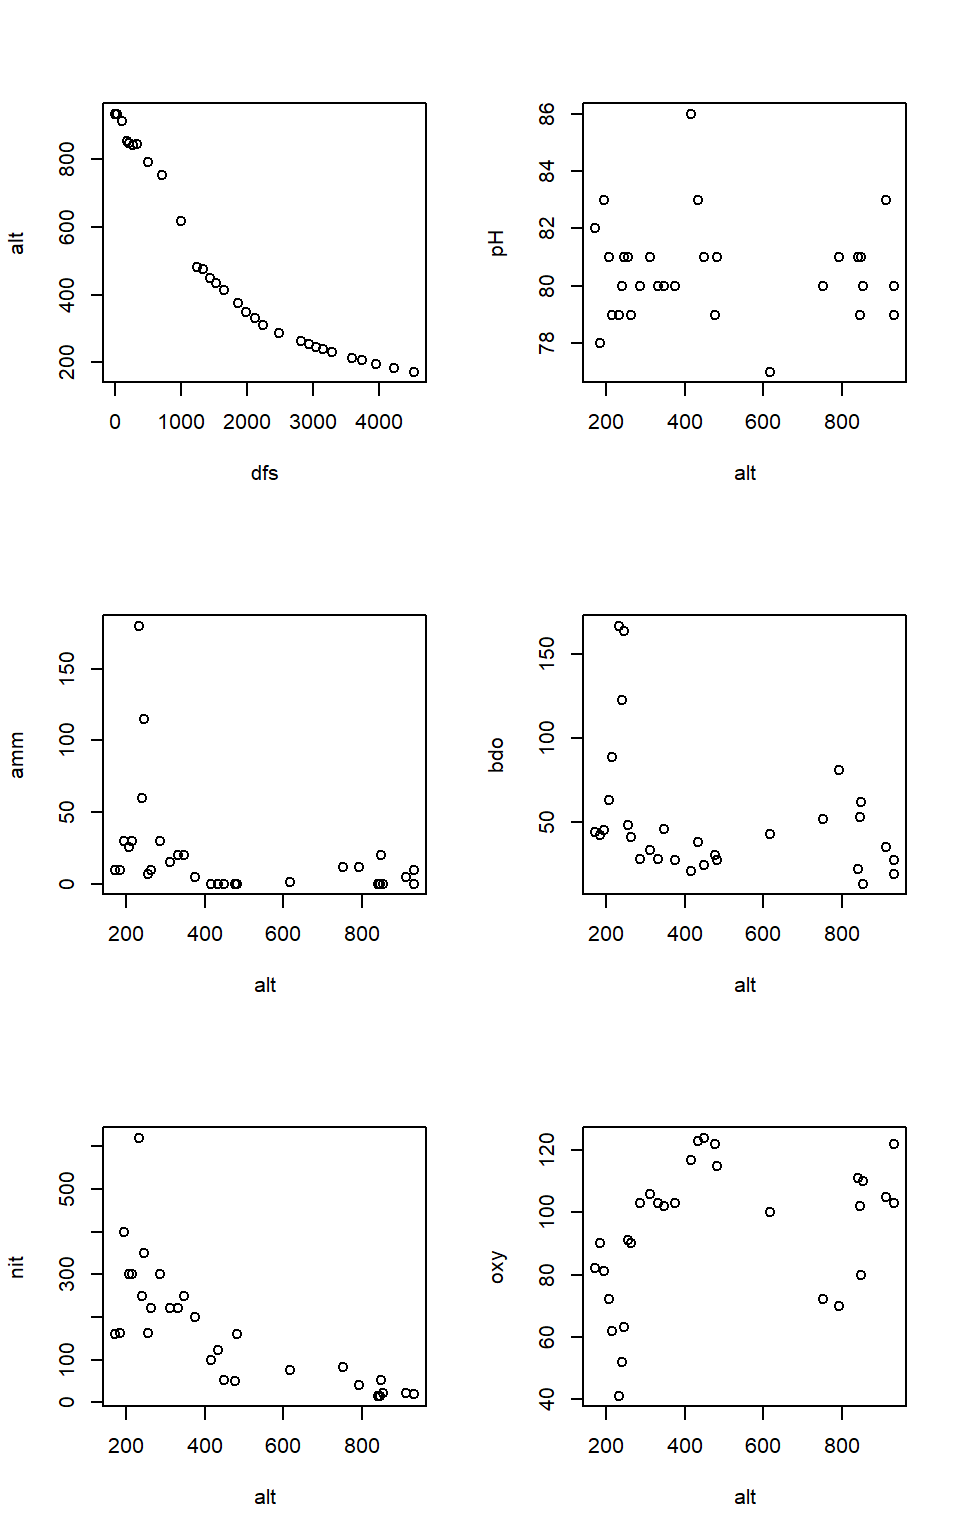
\includegraphics{IntroR_files/figure-latex/unnamed-chunk-124-1} \end{center}

\hypertarget{exportando-figuras-com-as-funuxe7uxf5es-png-tiff-jpeg-e-bmp}{%
\subsection{\texorpdfstring{Exportando figuras com as funções \texttt{png}, \texttt{tiff}, \texttt{jpeg} e \texttt{bmp}}{Exportando figuras com as funções png, tiff, jpeg e bmp}}\label{exportando-figuras-com-as-funuxe7uxf5es-png-tiff-jpeg-e-bmp}}

Temos melhor controle sobre a qualidade gráfica no R exportando figuras em uma variedade de formatos e resoluções. Exemplificamos esta funcionalidade abaixo com a função \texttt{png}. No entanto, uma breve busca nos menus de ajuda mostrará que existem funções similares para outras extensões de imagem que possume funcionamentos similares.

\begin{Shaded}
\begin{Highlighting}[]
\FunctionTok{png}\NormalTok{(}\AttributeTok{filename =} \StringTok{"Exemplo\_figura.png"}\NormalTok{,}
    \AttributeTok{width =} \DecValTok{15}\NormalTok{, }\AttributeTok{height =} \DecValTok{15}\NormalTok{, }\AttributeTok{units =} \StringTok{"cm"}\NormalTok{, }
    \AttributeTok{pointsize =} \DecValTok{10}\NormalTok{, }\AttributeTok{bg =} \StringTok{"white"}\NormalTok{, }\AttributeTok{res =} \DecValTok{800}\NormalTok{)}

\FunctionTok{plot}\NormalTok{(alt }\SpecialCharTok{\textasciitilde{}}\NormalTok{ dfs, }\AttributeTok{data =}\NormalTok{ ambiente, }\AttributeTok{pch =} \DecValTok{19}\NormalTok{, }\AttributeTok{type =} \StringTok{"b"}\NormalTok{, }
     \AttributeTok{xlab =} \StringTok{"Vazão"}\NormalTok{, }\AttributeTok{ylab =} \StringTok{"Elevação"}\NormalTok{)}

\FunctionTok{dev.off}\NormalTok{()}
\end{Highlighting}
\end{Shaded}

Lembre-se que a figura foi salva do diretório atual de sua seção de trabalho. Você pode conferir este diretório com:

\begin{Shaded}
\begin{Highlighting}[]
\FunctionTok{getwd}\NormalTok{()}
\end{Highlighting}
\end{Shaded}

Experimente alterar os argumentos \texttt{width}, \texttt{height}, \texttt{pointsize}, \texttt{units} (com \texttt{"px"}, \texttt{"in"}, \texttt{"cm"} ou \texttt{"mm"}) e \texttt{res}.

As capacidades gráficas no R incluem ainda muitos outros argumentos. Alguns deles são: cores (\texttt{col}), tipos da fonte (\texttt{font}), tamanhos de símbolos (\texttt{cex}), dos labels (\texttt{cex.lab}), dos rótulos dos eixos (\texttt{cex.axis}), título (\texttt{main}), etc. Pode-se ainda inserir legendas (função \texttt{legend}) e textos (função \texttt{text}). Veja o \textbf{help} de cada uma destas funções e a lista de argumentos possíveis para o ambiente gráfico do R em \texttt{?par}. Veja também uma demonstração com \texttt{demo(graphics)}, \texttt{demo(image)}, \texttt{demo(persp)} e \texttt{demo(plotmath)}.

Existem diversos outros pacotes gráficos além do \texttt{graphics}:

\begin{itemize}
\tightlist
\item
  \texttt{ggplot2}
\item
  \texttt{ggvis}
\item
  \texttt{Lattice}
\item
  \texttt{highcharter}
\item
  \texttt{Leaflet}
\item
  \texttt{RColorBrewer}
\item
  \texttt{Plotly}
\item
  \texttt{sunburstR}
\item
  \texttt{RGL}
\item
  \texttt{dygraphs}
\end{itemize}

Veremos somente uma introdução ao pacote \texttt{ggplot2} no capítulo \ref{tidy}. Você pode buscar informações nos manuais oficias destes pacotes, mas sem dúvida a fonte mais extensa de informação são todos os usuários que dispõem de seus exemplos na rede. Assim, para aprender sobre estes pacotes ou outras técinicas gráficas no R não exite em tentar um \textbf{Google} do tipo \href{https://www.google.com.br/search?sxsrf=ALeKk00KUMfabSYS-mRTqdTiLdeOR65jnA\%3A1594162286064\&source=hp\&ei=bvwEX8TUAZm25OUP0LCXsAw\&q=quero+fazer+meus+gr\%C3\%A1ficos+no+R\&oq=quero+fazer+meus+gr\%C3\%A1ficos+no+R\&gs_lcp=CgZwc3ktYWIQA1DwDVjwDWCRF2gAcAB4AIABmgGIAZoBkgEDMC4xmAEAoAECoAEBqgEHZ3dzLXdpeg\&sclient=psy-ab\&ved=0ahUKEwjEw5emnbzqAhUZG7kGHVDYBcYQ4dUDCAc\&uact=5}{quero fazer meus gráficos no R}.

\textbf{Boa sorte!!}

\hypertarget{part-uma-coleuxe7uxe3o-integrada-de-pacotes-para-ciuxeancia-de-dados}{%
\part{Uma coleção integrada de pacotes para ciência de dados}\label{part-uma-coleuxe7uxe3o-integrada-de-pacotes-para-ciuxeancia-de-dados}}

\hypertarget{tidy}{%
\chapter{\texorpdfstring{Os pacotes em \texttt{tidyverse}}{Os pacotes em tidyverse}}\label{tidy}}

A Ciência de Dados, como chamada atualmente, passa por uma coleção de ações relacionadas à importação de dados, formatação, padronização de informações, visualização, modelagem e comunicação dos resultados. Ainda que estes processos sejam conhecidos e aplicados por profissionais de diferentes áreas na academia ou no mercado, o uso cada vez mais recorrente do termo \textbf{Ciência de Dados} impulsionou a construção de ferramentas em diferentes linguagems de programação para integrar estes processos de forma coesa. No R, o pacote que trás esta filosofia em sua estrutura é o \texttt{tidyverse}. O \texttt{tidyverse} na realidade, agrega um \emph{conjunto de pacotes} que funcionam de maneira integrada. Atualmente (versão \texttt{1.3.1} em \texttt{2021-05-18}) estão incorporados no \texttt{tidyverse} os pacotes:

\begin{itemize}
\tightlist
\item
  \texttt{readr}: importação de dados
\item
  \texttt{dplyr}: manipulação de dados
\item
  \texttt{tidyr}: organização de dados
\item
  \texttt{purr}: programaçao funcional
\item
  \texttt{tibble}: visualização de data frames
\item
  \texttt{stringr}: manipulação de texto
\item
  \texttt{forcats}: manipulação de fatores
\item
  \texttt{ggplot2}: visualização gráfica
\end{itemize}

Além destes existem ainda outros que se integram bem à filosofia do \texttt{tidyverse} como o \texttt{lubridade} (manipulação de datas), o \texttt{readxl} (leitura de arquivos \texttt{.xls} e \texttt{.xlsx}), \texttt{rvest} (manipulação na web), o \texttt{rmarkdown} (formatação de relatórios dinâmicos, apesentações e outros documentos). Não iremos ver exemplos de todos os pacotes, somentes algumas das funções mais úteis. Você pode buscar mais informações sobre cada um deles no site do \href{https://www.tidyverse.org/packages/}{tidyverse}. Para uma visão geral de cada pacote, você pode verificar as \href{https://rstudio.com/resources/cheatsheets/}{Cheatsheets} que oferecem um resumo sobre as funções de diversos pacotes.

\hypertarget{instalando-os-pacotes-tidyverse}{%
\subsection{\texorpdfstring{Instalando os pacotes \texttt{tidyverse}}{Instalando os pacotes tidyverse}}\label{instalando-os-pacotes-tidyverse}}

Um \textbf{pacote} no R, trás um conjunto de funções organizadas ao redor de um problema comum. Você pode instalar um pacote no R de três formas:

\begin{itemize}
\tightlist
\item
  Utilizando o comando \texttt{install.packages("nome\_do\_pacote")} que irá buscá-lo no \(\texttt{CRAN}\), \href{https://cran.r-project.org/}{Comprehensive R Archive Network};
\item
  a partir do Github: ```devtools::install\_github(``nome\_do\_repositorio/nome\_do\_pacote'')
\item
  A partir de um arquivo compactado \texttt{.zip} ou \texttt{tar.gz} com o comando \texttt{install.packages("C:/seu\_diretorio/nome\_do\_pacote",\ repos\ =\ NULL)}
\end{itemize}

\begin{quote}
Lembre-se ao utilizar a segunda opção que o \href{https://cran.r-project.org/web/packages/devtools/index.html}{devtools} também é um pacote e portanto, deve ser instalado no R. Alguns pacotes não disponíveis no site oficial do \(\texttt{CRAN}\), \href{https://cran.r-project.org/}{Comprehensive R Archive Network} podem ser instalados somente por esta opção.
\end{quote}

Cada um dos pacotes incorporados no \texttt{tidyverse} pode ser instalado individualmente. Por exemplo:

\begin{Shaded}
\begin{Highlighting}[]
\FunctionTok{install.packages}\NormalTok{(}\StringTok{"dplyr"}\NormalTok{)}
\FunctionTok{install.packages}\NormalTok{(}\StringTok{"ggplot2"}\NormalTok{)}
\end{Highlighting}
\end{Shaded}

Entretando, ao instalar o \texttt{tidyverse}, todos são instalados de uma única vez:

\begin{Shaded}
\begin{Highlighting}[]
\FunctionTok{install.packages}\NormalTok{(}\StringTok{"tidyverse"}\NormalTok{)}
\end{Highlighting}
\end{Shaded}

\hypertarget{carregando-os-pacotes}{%
\section{Carregando os pacotes}\label{carregando-os-pacotes}}

Ao iniciar uma seção, você deve sempre carregar os pacotes que irá utilizar. No caso do \texttt{tidyverse}, você pode carregar cada pacote individualmente:

\begin{Shaded}
\begin{Highlighting}[]
\FunctionTok{library}\NormalTok{(dplyr)}
\FunctionTok{library}\NormalTok{(ggplot2)}
\end{Highlighting}
\end{Shaded}

Ou todos de uma única vez:

\begin{Shaded}
\begin{Highlighting}[]
\FunctionTok{library}\NormalTok{(tidyverse)}
\end{Highlighting}
\end{Shaded}

\hypertarget{importe}{%
\chapter{Importando/Exportando dados}\label{importe}}

\hypertarget{ajustando-o-diretuxf3rio-de-trabalho}{%
\section{Ajustando o diretório de trabalho}\label{ajustando-o-diretuxf3rio-de-trabalho}}

Antes de apresentarmos as funções de importação e exportação de dados devemos re-lembrar as funções que nos permitem verificar e alterar o \emph{diretório de trabalho}. Um diretório de trabalho é que o local onde o R irá buscar e salvar arquivos em seu computador. Se não for definido, o R irá utilizar o diretório base. No R-Studio você pode verificar qual é seu diretório base no menu: \texttt{Tools\ -\/-\textgreater{}\ Global\ Options\ -\/-\textgreater{}\ R\ General}.

Se você estiver utilizando um \textbf{projeto} o R irá utilizar o diretório onde está o arquivo com extensão \texttt{.Rproj} . Uma das vantagens em utilizar \emph{projetos} no R é a facilidade em manipular o diretório de trabalho e sub-diretórios dentro deles. Sub-diretórios dentro da pasta de um projeto podem auxiliar na organização das base de dados para importação, do material gerado como figuras, slides, arquivos \texttt{.pdf}, etc. No R-Studio você pode criar um projeto via menu: \texttt{File\ -\/-\textgreater{}\ New\ Project...}.

Você pode verificar seu diretório de trabalho com a função \texttt{getwd()}. Esta função não requer argumentos. A função \texttt{setwd()} é utilizada para alterar o diretório de trabalho e recebe como argumento o diretório de destino. O comando:

\begin{Shaded}
\begin{Highlighting}[]
\FunctionTok{getwd}\NormalTok{(}\StringTok{"C:/seu\_caminho/IntroR"}\NormalTok{)}
\end{Highlighting}
\end{Shaded}

Irá alterar o caminho de busca para esta pasta.

\hypertarget{importando-dados-em-arquvos-de-texto}{%
\section{Importando dados em arquvos de texto}\label{importando-dados-em-arquvos-de-texto}}

O pacote responsável pela importação de dados no \texttt{tidyverse} é o \texttt{readr}. Este pacote permite importar arquivos de texto no formato \texttt{.csv} ou \texttt{.txt}.

Existem diversas funções no pacote \texttt{readr}. Veja seu manual \href{https://cran.r-project.org/web/packages/readr/index.html}{Aqui}. A função \texttt{read\_csv()} importa arquivos texto em que as colunas são separadas por \emph{vírgulas}. A função \texttt{read\_tsv()} importa arquivos texto em que as colunas são separadas por \emph{tabulações}. Iremos ver a função \texttt{read\_delim()} que é mais geral e permite que você especifique o tipo de separador (\emph{delimitador}) de acordo com o padrão em seu arquivo. Os delimitadores mais comuns são \emph{vírgulas}, \emph{tabulações} ou \emph{ponto-e-vírgula}.

Vamos voltar ao arquivo \texttt{doubs\_environment.csv} visto no capítulo \ref{manipulacao}. Vamos importá-lo agora utilizando a função \texttt{read\_delim()}.

\begin{Shaded}
\begin{Highlighting}[]
\FunctionTok{library}\NormalTok{(readr)}
\end{Highlighting}
\end{Shaded}

\begin{Shaded}
\begin{Highlighting}[]
\NormalTok{dbenv }\OtherTok{=} \FunctionTok{read\_delim}\NormalTok{(}\AttributeTok{file =} \StringTok{"C:/seu\_caminho/IntroR/dbenv.csv"}\NormalTok{, }\AttributeTok{delim =} \StringTok{","}\NormalTok{)}
\end{Highlighting}
\end{Shaded}

verifique o objeto importado.

\begin{Shaded}
\begin{Highlighting}[]
\NormalTok{dbenv}
\end{Highlighting}
\end{Shaded}

\begin{verbatim}
## # A tibble: 30 x 11
##      dfs   alt   slo   flo    pH   har   pho   nit   amm   oxy   bdo
##    <dbl> <dbl> <dbl> <dbl> <dbl> <dbl> <dbl> <dbl> <dbl> <dbl> <dbl>
##  1     3   934  6.18    84    79    45     1    20     0   122    27
##  2    22   932  3.43   100    80    40     2    20    10   103    19
##  3   102   914  3.64   180    83    52     5    22     5   105    35
##  4   185   854  3.50   253    80    72    10    21     0   110    13
##  5   215   849  3.18   264    81    84    38    52    20    80    62
##  6   324   846  3.50   286    79    60    20    15     0   102    53
##  7   268   841  4.20   400    81    88     7    15     0   111    22
##  8   491   792  3.26   130    81    94    20    41    12    70    81
##  9   705   752  2.56   480    80    90    30    82    12    72    52
## 10   990   617  4.61  1000    77    82     6    75     1   100    43
## # ... with 20 more rows
\end{verbatim}

O objeto é do tipo \texttt{tibble} com 30 linhas por 11 colunas. Note que dependendo do tamanho de sua janela, nem todas as linhas e colunas irão aparecer, porém será indicado as linhas e colunas ocultas.

\hypertarget{pipe}{%
\chapter{Operador Pipe}\label{pipe}}

O \textbf{operador pipe} (\texttt{\%\textgreater{}\%}) é um facilitador para a manipulação e formatação de dados na filosofia \emph{tidyverse}. O operador pipe não precisa ser utilizado somente com as funções dos pacotes do tidyverse, pode ser utilizado com qualquer função em R. Sua função é facilitar a leitura de códigos, sobretudo códigos longos de formatação de data frames.

Para utilizá-lo instale e carrege o pacote \texttt{magrittr}:

\begin{Shaded}
\begin{Highlighting}[]
\FunctionTok{install.packages}\NormalTok{(}\StringTok{"magrittr"}\NormalTok{)}
\FunctionTok{library}\NormalTok{(magrittr)}
\end{Highlighting}
\end{Shaded}

Este operador funciona fazendo com que um objeto criado ao lado esquerdo de uma expressão, seja utilizado como \emph{entrada} de uma função escrita ao lado direito da expressão conforme:

\(y\) \%\textgreater\% \(f(y)\)

Veja um exemplo:

\begin{Shaded}
\begin{Highlighting}[]
\NormalTok{variavel }\OtherTok{\textless{}{-}} \DecValTok{49}
\NormalTok{variavel }\SpecialCharTok{\%\textgreater{}\%} \FunctionTok{sqrt}\NormalTok{()}
\end{Highlighting}
\end{Shaded}

\begin{verbatim}
## [1] 7
\end{verbatim}

O objeto \texttt{variavel} às esquerda de \textbf{\%\textgreater\%} é portanto utilizado como entrada para a função \texttt{sqrt()}, à direita de \textbf{\%\textgreater\%}. A expressão é similar a:

\begin{Shaded}
\begin{Highlighting}[]
\NormalTok{variavel }\OtherTok{\textless{}{-}} \DecValTok{49}
\FunctionTok{sqrt}\NormalTok{(variavel)}
\end{Highlighting}
\end{Shaded}

\begin{verbatim}
## [1] 7
\end{verbatim}

Neste exemplo, o uso do operador pipe não trás qualquer vantagem. Por outro lado veja a sequência abaixo escrita da forma convencional:

\begin{Shaded}
\begin{Highlighting}[]
\NormalTok{objeto }\OtherTok{\textless{}{-}} \FunctionTok{c}\NormalTok{(}\DecValTok{2}\NormalTok{,}\DecValTok{6}\NormalTok{,}\DecValTok{3}\NormalTok{,}\DecValTok{8}\NormalTok{,}\DecValTok{10}\NormalTok{)}
\FunctionTok{sum}\NormalTok{(}\FunctionTok{diff}\NormalTok{(}\FunctionTok{round}\NormalTok{(}\FunctionTok{sqrt}\NormalTok{(objeto),}\AttributeTok{digits =} \DecValTok{2}\NormalTok{)))}
\end{Highlighting}
\end{Shaded}

\begin{verbatim}
## [1] 1.75
\end{verbatim}

E utilizando o operador pipe:

\begin{Shaded}
\begin{Highlighting}[]
\NormalTok{objeto }\OtherTok{\textless{}{-}} \FunctionTok{c}\NormalTok{(}\DecValTok{2}\NormalTok{,}\DecValTok{6}\NormalTok{,}\DecValTok{3}\NormalTok{,}\DecValTok{8}\NormalTok{,}\DecValTok{10}\NormalTok{)}

\NormalTok{objeto }\SpecialCharTok{\%\textgreater{}\%} \FunctionTok{sqrt}\NormalTok{() }\SpecialCharTok{\%\textgreater{}\%} \FunctionTok{round}\NormalTok{(}\AttributeTok{digits =} \DecValTok{2}\NormalTok{) }\SpecialCharTok{\%\textgreater{}\%} \FunctionTok{diff}\NormalTok{() }\SpecialCharTok{\%\textgreater{}\%} \FunctionTok{sum}\NormalTok{()}
\end{Highlighting}
\end{Shaded}

\begin{verbatim}
## [1] 1.75
\end{verbatim}

Na forma convencional, a leitura se dá de \textbf{dentro para fora} da expressão. À medida que o número de operações aumenta, a leitura e consequentemente a correção desta sequência se torna complexa.

Utilizando o operador pipe a leitura se dá:

\begin{enumerate}
\def\labelenumi{\arabic{enumi}.}
\item
  Pegue o objeto \texttt{variável};
\item
  Tire a raiz quadrada;
\item
  Arredonde a raiz quadrada para duas casa decimais;
\item
  Calcule a diferença de um objeto com o anterior; e
\item
  Some as entradas.
\end{enumerate}

Por hora, busque entender esta sequência. As vantagens do operador pipe se tornarão mais claras quando formos falar de formatação de data frames nos capítulos a frente.

\hypertarget{format}{%
\chapter{Manipulação e formatação de dados}\label{format}}

Após importar uma basde de dados para o R, os principais pacotes para manipulação e formatação de data frames são o \texttt{dplyr} e o \texttt{tidyr}. As funções destes pacotes oferecem uma etapa inicial na análise, modelagem e comunicação de dados. Lembramos aqui que uma base de dados é organizada em um formato de tabela em que as linhas são as \emph{observações} e as colunas são as \emph{variáveis} que descrevem estas observações. Estas variáveis podem ser quantitativas (contínuas ou discretas) ou qualitativas (ordenadas ou não).

\hypertarget{transformauxe7uxe3o-de-dados-os-pacotes-dplyr-e-tidyr}{%
\section{\texorpdfstring{Transformação de dados: os pacotes \texttt{dplyr} e \texttt{tidyr}}{Transformação de dados: os pacotes dplyr e tidyr}}\label{transformauxe7uxe3o-de-dados-os-pacotes-dplyr-e-tidyr}}

Aqui veremos funções principais para manipular as observações nas linhas (\emph{Manipulate Cases}), manipular descritores nas colunas (\emph{Manipulate Variables}) e combinar tabelas (\emph{Combine Tables}). Na \href{https://rstudio.com/resources/cheatsheets/}{Cheatsheets} do \texttt{dplyr} você verá também a variedade de funções relacionadas ao cáculo sobre vetores (\emph{Vector Functions}), funções resumo (\emph{Summary Functions}, e \emph{Summarise Cases}) e manipulação de nomes das linhas.

\hypertarget{ordenando-as-linhas-funuxe7uxf5es-arrange-e-desc}{%
\subsection{\texorpdfstring{Ordenando as linhas: funções \texttt{arrange()} e \texttt{desc()}}{Ordenando as linhas: funções arrange() e desc()}}\label{ordenando-as-linhas-funuxe7uxf5es-arrange-e-desc}}

Estas funções permitem que você ordene a base de dados seguindo os valores de alguma de suas colunas. Vamos utilizar como exemplo a base de dados \texttt{iris} comumente utilizadas em uma variedade de tutorias sobre ciência de dados. Carrege e verifique a base de dados composta por 150 linhas e 5 colunas.

\begin{Shaded}
\begin{Highlighting}[]
\FunctionTok{data}\NormalTok{(}\StringTok{"iris"}\NormalTok{)}
\FunctionTok{head}\NormalTok{(iris, }\DecValTok{10}\NormalTok{)}
\end{Highlighting}
\end{Shaded}

Vamos ordenar a tabela pela coluna \texttt{Sepal.Length}.

\begin{Shaded}
\begin{Highlighting}[]
\NormalTok{iris }\SpecialCharTok{\%\textgreater{}\%} 
  \FunctionTok{arrange}\NormalTok{(Sepal.Length)}
\end{Highlighting}
\end{Shaded}

\begin{verbatim}
##    Sepal.Length Sepal.Width Petal.Length Petal.Width Species
## 1           4.3         3.0          1.1         0.1  setosa
## 2           4.4         2.9          1.4         0.2  setosa
## 3           4.4         3.0          1.3         0.2  setosa
## 4           4.4         3.2          1.3         0.2  setosa
## 5           4.5         2.3          1.3         0.3  setosa
## 6           4.6         3.1          1.5         0.2  setosa
## 7           4.6         3.4          1.4         0.3  setosa
## 8           4.6         3.6          1.0         0.2  setosa
## 9           4.6         3.2          1.4         0.2  setosa
## 10          4.7         3.2          1.3         0.2  setosa
\end{verbatim}

As linhas aparecem agora de acordo com os valores (em ordem crescente) de \texttt{Sepal.Length}, iniciando em 4.3.

Em seguida faça o mesmo em ordem \emph{decresente}.

\begin{Shaded}
\begin{Highlighting}[]
\NormalTok{iris }\SpecialCharTok{\%\textgreater{}\%} 
  \FunctionTok{arrange}\NormalTok{(}\FunctionTok{desc}\NormalTok{(Sepal.Length))}
\end{Highlighting}
\end{Shaded}

Podemos combinar duas colunas, ordenando a tabela em função da coluna \texttt{Species} (em ordem alfabética decrescente) e em função de \texttt{Sepal.Length} (em ordem crescente).

\begin{Shaded}
\begin{Highlighting}[]
\NormalTok{iris }\SpecialCharTok{\%\textgreater{}\%} 
  \FunctionTok{arrange}\NormalTok{(}\FunctionTok{desc}\NormalTok{(Species), Sepal.Length)}
\end{Highlighting}
\end{Shaded}

Nos exemplos acimas, somente visualizamos a tabela em diferentes ordens. Se quisermos criar um novo objeto com a tabela em alguma destas sequências fazemos:

\begin{Shaded}
\begin{Highlighting}[]
\NormalTok{iris\_ordenado }\OtherTok{\textless{}{-}}\NormalTok{ iris }\SpecialCharTok{\%\textgreater{}\%} 
  \FunctionTok{arrange}\NormalTok{(Sepal.Length)}

\NormalTok{iris\_ordenado}
\end{Highlighting}
\end{Shaded}

\begin{verbatim}
##   Sepal.Length Sepal.Width Petal.Length Petal.Width Species
## 1          4.3         3.0          1.1         0.1  setosa
## 2          4.4         2.9          1.4         0.2  setosa
## 3          4.4         3.0          1.3         0.2  setosa
## 4          4.4         3.2          1.3         0.2  setosa
## 5          4.5         2.3          1.3         0.3  setosa
## 6          4.6         3.1          1.5         0.2  setosa
\end{verbatim}

\hypertarget{filtrando-linhas-funuxe7uxe3o-filter}{%
\subsection{\texorpdfstring{Filtrando linhas: função \texttt{filter()}}{Filtrando linhas: função filter()}}\label{filtrando-linhas-funuxe7uxe3o-filter}}

Esta função permite extrair somente as linhas de uma tabela que satisfaçam uma condição lógica. Vamos extrair as linhas referentes à espécie \texttt{virginica}.

\begin{Shaded}
\begin{Highlighting}[]
\NormalTok{iris }\SpecialCharTok{\%\textgreater{}\%} 
  \FunctionTok{filter}\NormalTok{(Species }\SpecialCharTok{==} \StringTok{"virginica"}\NormalTok{)}
\end{Highlighting}
\end{Shaded}

Ou às espécies \emph{diferentes} de \texttt{virginica}.

\begin{Shaded}
\begin{Highlighting}[]
\NormalTok{iris }\SpecialCharTok{\%\textgreater{}\%} 
  \FunctionTok{filter}\NormalTok{(Species }\SpecialCharTok{!=} \StringTok{"virginica"}\NormalTok{)}
\end{Highlighting}
\end{Shaded}

Agora, vamos filtrar as linhas em que o comprimento das pétalas seja menor que 1.3.

\begin{Shaded}
\begin{Highlighting}[]
\NormalTok{iris }\SpecialCharTok{\%\textgreater{}\%} 
  \FunctionTok{filter}\NormalTok{(Petal.Length }\SpecialCharTok{\textless{}} \FloatTok{1.3}\NormalTok{)}
\end{Highlighting}
\end{Shaded}

E para o comprimento das pétalas seja menor que 1.3 \textbf{E} o comprimento das sépalas maior ou igual a 5.

\begin{Shaded}
\begin{Highlighting}[]
\NormalTok{iris }\SpecialCharTok{\%\textgreater{}\%} 
  \FunctionTok{filter}\NormalTok{(Petal.Length }\SpecialCharTok{\textless{}} \FloatTok{1.3} \SpecialCharTok{\&}\NormalTok{ Sepal.Length }\SpecialCharTok{\textgreater{}=} \DecValTok{5}\NormalTok{)}
\end{Highlighting}
\end{Shaded}

\hypertarget{selecionando-colunas-funuxe7uxe3o-select}{%
\subsection{\texorpdfstring{Selecionando colunas: função \texttt{select()}}{Selecionando colunas: função select()}}\label{selecionando-colunas-funuxe7uxe3o-select}}

A função select permite extrair ou reorganizar um subconjunto colunas de um data frame. Rode os exemplos a seguir:

\begin{Shaded}
\begin{Highlighting}[]
\NormalTok{iris }\SpecialCharTok{\%\textgreater{}\%} 
  \FunctionTok{select}\NormalTok{(Petal.Length)}
\end{Highlighting}
\end{Shaded}

\begin{Shaded}
\begin{Highlighting}[]
\NormalTok{iris }\SpecialCharTok{\%\textgreater{}\%} 
  \FunctionTok{select}\NormalTok{(Petal.Length, Species)}
\end{Highlighting}
\end{Shaded}

\begin{Shaded}
\begin{Highlighting}[]
\NormalTok{iris }\SpecialCharTok{\%\textgreater{}\%} 
  \FunctionTok{select}\NormalTok{(Petal.Length}\SpecialCharTok{:}\NormalTok{Species)}
\end{Highlighting}
\end{Shaded}

\begin{Shaded}
\begin{Highlighting}[]
\NormalTok{iris }\SpecialCharTok{\%\textgreater{}\%} 
  \FunctionTok{select}\NormalTok{(Species}\SpecialCharTok{:}\NormalTok{Petal.Length)}
\end{Highlighting}
\end{Shaded}

\begin{Shaded}
\begin{Highlighting}[]
\NormalTok{iris }\SpecialCharTok{\%\textgreater{}\%} 
  \FunctionTok{select}\NormalTok{(}\SpecialCharTok{!}\FunctionTok{c}\NormalTok{(Petal.Length, Species))}
\end{Highlighting}
\end{Shaded}

\begin{Shaded}
\begin{Highlighting}[]
\NormalTok{iris }\SpecialCharTok{\%\textgreater{}\%} 
  \FunctionTok{select}\NormalTok{(}\FunctionTok{starts\_with}\NormalTok{(}\StringTok{"Sepal"}\NormalTok{))}
\end{Highlighting}
\end{Shaded}

Finalmente, combine as funções \texttt{filter()} e \texttt{select()} para extrair um subconjunto do data frame:

\begin{Shaded}
\begin{Highlighting}[]
\NormalTok{iris }\SpecialCharTok{\%\textgreater{}\%} 
  \FunctionTok{select}\NormalTok{(}\FunctionTok{starts\_with}\NormalTok{(}\StringTok{"Sepal"}\NormalTok{)) }\SpecialCharTok{\%\textgreater{}\%} 
  \FunctionTok{filter}\NormalTok{(Sepal.Length }\SpecialCharTok{\textless{}=} \FloatTok{4.5}\NormalTok{)}
\end{Highlighting}
\end{Shaded}

\hypertarget{agrupando-tabelas-funuxe7uxf5es-do-grupo-join}{%
\subsection{\texorpdfstring{Agrupando tabelas: funções do grupo \texttt{join}}{Agrupando tabelas: funções do grupo join}}\label{agrupando-tabelas-funuxe7uxf5es-do-grupo-join}}

Se você tem alguma experiência em linguagem SQL para banco de dados, irá compreender facilmente o uso do grupo de funções \textbf{join}. Veremos aqui as funções \texttt{left\_join()}, \texttt{right\_join()}, \texttt{inner\_join()} e \texttt{anti\_join()}.

Considere as duas tabelas abaixo que podem ser acessadas em Regiao.csv e Habitat.csv

\begin{verbatim}
## # A tibble: 10 x 4
##    Riacho Bacia      Município      Área
##    <chr>  <chr>      <chr>         <dbl>
##  1 R1     Boicucanga São Sebastião  30.3
##  2 R4     Boicucanga São Sebastião  30.3
##  3 R8     Boicucanga São Sebastião  30.3
##  4 R2     Cubatão    Cubatão       189  
##  5 R5     Cubatão    Cubatão       189  
##  6 R10    Cubatão    Cubatão       189  
##  7 R13    Cubatão    Cubatão       189  
##  8 R6     Quilombo   Santos         86  
##  9 R9     Quilombo   Santos         86  
## 10 R7     Quilombo   Santos         86
\end{verbatim}

\begin{verbatim}
## # A tibble: 8 x 4
##   Riacho Altitude Largura Profundidade
##   <chr>     <dbl>   <dbl>        <dbl>
## 1 R1           74     7.8         20.2
## 2 R4           14    10.9         17.7
## 3 R8          245     8.3         19.5
## 4 R11         241     2.2         20.3
## 5 R2           29     1.6         11.8
## 6 R6           86    15.2         35.3
## 7 R9           77     4.1         18.9
## 8 R7           63    14.2         42.1
\end{verbatim}

\begin{Shaded}
\begin{Highlighting}[]
\NormalTok{regiao }\OtherTok{\textless{}{-}} \FunctionTok{read\_csv}\NormalTok{(}\StringTok{"C:/seu\_caminho/IntroR/Regiao.csv"}\NormalTok{)}
\NormalTok{regiao}
\end{Highlighting}
\end{Shaded}

\begin{Shaded}
\begin{Highlighting}[]
\NormalTok{habitat }\OtherTok{\textless{}{-}} \FunctionTok{read\_csv}\NormalTok{(}\StringTok{"C:/seu\_caminho/IntroR/Habitat.csv"}\NormalTok{)}
\NormalTok{habitat}
\end{Highlighting}
\end{Shaded}

A tabela \texttt{regiao}, contém informações sobre alguns o bacia hidrográfica, á área da bacia e o múnicípio de alguns riachos da região litorânea do estado de São Paulo. A tabela \texttt{trecho}, contém informações sobre a largura e profundidades destes riachos. Alguns riachos são coumuns às duas tabelas, enquanto outros ocorrem somente em uma ou em outra tabela. Sabendo que a coluna \texttt{Riacho} (R1, R2, R3,\ldots.R13) se referem ao mesmo ponto de amostragem, podemos utilizá-la para \textbf{combinar} as informações das duas tabelas.

\hypertarget{funuxe7uxe3o-left_join}{%
\subsubsection{\texorpdfstring{Função \texttt{left\_join()}}{Função left\_join()}}\label{funuxe7uxe3o-left_join}}

Retorna todas as linhas da tabela à \textbf{esquerda} as as colunas das duas tabelas. Linhas sem correspondência na tabela da direita terão valores de \texttt{NA}. Se houver várias correspondências, todas as combinações serão retornadas.

\begin{Shaded}
\begin{Highlighting}[]
\NormalTok{regiao }\SpecialCharTok{\%\textgreater{}\%} \FunctionTok{left\_join}\NormalTok{(}\AttributeTok{y =}\NormalTok{ habitat)}
\end{Highlighting}
\end{Shaded}

\begin{verbatim}
## # A tibble: 10 x 7
##    Riacho Bacia      Município      Área Altitude Largura Profundidade
##    <chr>  <chr>      <chr>         <dbl>    <dbl>   <dbl>        <dbl>
##  1 R1     Boicucanga São Sebastião  30.3       74     7.8         20.2
##  2 R4     Boicucanga São Sebastião  30.3       14    10.9         17.7
##  3 R8     Boicucanga São Sebastião  30.3      245     8.3         19.5
##  4 R2     Cubatão    Cubatão       189         29     1.6         11.8
##  5 R5     Cubatão    Cubatão       189         NA    NA           NA  
##  6 R10    Cubatão    Cubatão       189         NA    NA           NA  
##  7 R13    Cubatão    Cubatão       189         NA    NA           NA  
##  8 R6     Quilombo   Santos         86         86    15.2         35.3
##  9 R9     Quilombo   Santos         86         77     4.1         18.9
## 10 R7     Quilombo   Santos         86         63    14.2         42.1
\end{verbatim}

Veja que \textbf{todas} as linhas da tabela \texttt{regiao} estão presentes. Foram adicionadas a elas as informações de \texttt{Altitude}, \texttt{Largura} e \texttt{Profundidade}, somente para os riachos que também estavam presentes na tabela \texttt{habitat}.

\hypertarget{funuxe7uxe3o-right_join}{%
\subsubsection{\texorpdfstring{Função \texttt{right\_join()}}{Função right\_join()}}\label{funuxe7uxe3o-right_join}}

Retorna todas as linhas da tabela à \textbf{direita} as as colunas das duas tabelas. Linhas sem correspondência na tabela da esquerda terão valores de \texttt{NA}. Se houver várias correspondências, todas as combinações serão retornadas.

\begin{Shaded}
\begin{Highlighting}[]
\NormalTok{regiao }\SpecialCharTok{\%\textgreater{}\%} \FunctionTok{right\_join}\NormalTok{(}\AttributeTok{y =}\NormalTok{ habitat)}
\end{Highlighting}
\end{Shaded}

\begin{verbatim}
## # A tibble: 8 x 7
##   Riacho Bacia      Município      Área Altitude Largura Profundidade
##   <chr>  <chr>      <chr>         <dbl>    <dbl>   <dbl>        <dbl>
## 1 R1     Boicucanga São Sebastião  30.3       74     7.8         20.2
## 2 R4     Boicucanga São Sebastião  30.3       14    10.9         17.7
## 3 R8     Boicucanga São Sebastião  30.3      245     8.3         19.5
## 4 R2     Cubatão    Cubatão       189         29     1.6         11.8
## 5 R6     Quilombo   Santos         86         86    15.2         35.3
## 6 R9     Quilombo   Santos         86         77     4.1         18.9
## 7 R7     Quilombo   Santos         86         63    14.2         42.1
## 8 R11    <NA>       <NA>           NA        241     2.2         20.3
\end{verbatim}

Note que a coluna de \texttt{R11} contém \texttt{NA} nas colunas \texttt{Bacia} e \texttt{Município}, pois este riacho não está presente na tabela \texttt{regiao}.

\hypertarget{funuxe7uxe3o-inner_join}{%
\subsubsection{\texorpdfstring{Função \texttt{inner\_join()}}{Função inner\_join()}}\label{funuxe7uxe3o-inner_join}}

Resgata apenas as linhas coincidantes a \textbf{ambas} as tabelas.

\begin{Shaded}
\begin{Highlighting}[]
\NormalTok{regiao }\SpecialCharTok{\%\textgreater{}\%} \FunctionTok{inner\_join}\NormalTok{(}\AttributeTok{y =}\NormalTok{ habitat)}
\end{Highlighting}
\end{Shaded}

\hypertarget{funuxe7uxe3o-anti_join}{%
\subsubsection{\texorpdfstring{Função \texttt{anti\_join()}}{Função anti\_join()}}\label{funuxe7uxe3o-anti_join}}

Retorna todas as linhas da tabela à esquerda em que existem correspondências com a de direita. Retorna todas as colunas de ambas. Se houver várias correspondências, todas as combinações serão retornadas. Testes os comandos abaixo.

\begin{Shaded}
\begin{Highlighting}[]
\NormalTok{regiao }\SpecialCharTok{\%\textgreater{}\%} \FunctionTok{anti\_join}\NormalTok{(}\AttributeTok{y =}\NormalTok{ habitat)}
\end{Highlighting}
\end{Shaded}

\begin{Shaded}
\begin{Highlighting}[]
\NormalTok{habitat }\SpecialCharTok{\%\textgreater{}\%} \FunctionTok{anti\_join}\NormalTok{(}\AttributeTok{y =}\NormalTok{ regiao)}
\end{Highlighting}
\end{Shaded}

\hypertarget{funuxe7uxe3o-full_join}{%
\subsubsection{\texorpdfstring{Função \texttt{full\_join()}}{Função full\_join()}}\label{funuxe7uxe3o-full_join}}

Retorna todas as linhas e colunas das duas tabelas. Nas células em que não houver valores correspondentes, retorna \texttt{NA} na posição faltante.

\begin{Shaded}
\begin{Highlighting}[]
\NormalTok{regiao }\SpecialCharTok{\%\textgreater{}\%} \FunctionTok{full\_join}\NormalTok{(}\AttributeTok{y =}\NormalTok{ habitat)}
\end{Highlighting}
\end{Shaded}

\begin{Shaded}
\begin{Highlighting}[]
\NormalTok{habitat }\SpecialCharTok{\%\textgreater{}\%} \FunctionTok{semi\_join}\NormalTok{(}\AttributeTok{y =}\NormalTok{ regiao)}
\end{Highlighting}
\end{Shaded}

\hypertarget{criando-e-modificando-colunas-funuxe7uxe3o-mutate}{%
\subsection{\texorpdfstring{Criando e modificando colunas: função \texttt{mutate()}}{Criando e modificando colunas: função mutate()}}\label{criando-e-modificando-colunas-funuxe7uxe3o-mutate}}

Voltemos à base de dados Doubs river.

\begin{Shaded}
\begin{Highlighting}[]
\FunctionTok{library}\NormalTok{(ade4)}
\FunctionTok{data}\NormalTok{(doubs)}
\NormalTok{ambiente }\OtherTok{\textless{}{-}}\NormalTok{ doubs}\SpecialCharTok{$}\NormalTok{env}
\FunctionTok{head}\NormalTok{(ambiente)}
\end{Highlighting}
\end{Shaded}

\begin{verbatim}
##   dfs alt   slo flo pH har pho nit amm oxy bdo
## 1   3 934 6.176  84 79  45   1  20   0 122  27
## 2  22 932 3.434 100 80  40   2  20  10 103  19
## 3 102 914 3.638 180 83  52   5  22   5 105  35
## 4 185 854 3.497 253 80  72  10  21   0 110  13
## 5 215 849 3.178 264 81  84  38  52  20  80  62
## 6 324 846 3.497 286 79  60  20  15   0 102  53
\end{verbatim}

Veja que a coluna pH está dada em ph \(\times\) 10. Vamos retornar à escala unitária.

\begin{Shaded}
\begin{Highlighting}[]
\NormalTok{ambiente }\SpecialCharTok{\%\textgreater{}\%} 
  \FunctionTok{mutate}\NormalTok{(}\AttributeTok{pH =}\NormalTok{ pH}\SpecialCharTok{/}\DecValTok{10}\NormalTok{)}
\end{Highlighting}
\end{Shaded}

\begin{verbatim}
##     dfs alt   slo  flo  pH har pho nit amm oxy bdo
## 1     3 934 6.176   84 7.9  45   1  20   0 122  27
## 2    22 932 3.434  100 8.0  40   2  20  10 103  19
## 3   102 914 3.638  180 8.3  52   5  22   5 105  35
## 4   185 854 3.497  253 8.0  72  10  21   0 110  13
## 5   215 849 3.178  264 8.1  84  38  52  20  80  62
## 6   324 846 3.497  286 7.9  60  20  15   0 102  53
## 7   268 841 4.205  400 8.1  88   7  15   0 111  22
## 8   491 792 3.258  130 8.1  94  20  41  12  70  81
## 9   705 752 2.565  480 8.0  90  30  82  12  72  52
## 10  990 617 4.605 1000 7.7  82   6  75   1 100  43
## 11 1234 483 3.738 1990 8.1  96  30 160   0 115  27
## 12 1324 477 2.833 2000 7.9  86   4  50   0 122  30
## 13 1436 450 3.091 2110 8.1  98   6  52   0 124  24
## 14 1522 434 2.565 2120 8.3  98  27 123   0 123  38
## 15 1645 415 1.792 2300 8.6  86  40 100   0 117  21
## 16 1859 375 3.045 1610 8.0  88  20 200   5 103  27
## 17 1985 348 1.792 2430 8.0  92  20 250  20 102  46
## 18 2110 332 2.197 2500 8.0  90  50 220  20 103  28
## 19 2246 310 1.792 2590 8.1  84  60 220  15 106  33
## 20 2477 286 2.197 2680 8.0  86  30 300  30 103  28
## 21 2812 262 2.398 2720 7.9  85  20 220  10  90  41
## 22 2940 254 2.708 2790 8.1  88  20 162   7  91  48
## 23 3043 246 2.565 2880 8.1  97 260 350 115  63 164
## 24 3147 241 1.386 2976 8.0  99 140 250  60  52 123
## 25 3278 231 1.792 3870 7.9 100 422 620 180  41 167
## 26 3579 214 1.792 3910 7.9  94 143 300  30  62  89
## 27 3732 206 2.565 3960 8.1  90  58 300  26  72  63
## 28 3947 195 1.386 4320 8.3 100  74 400  30  81  45
## 29 4220 183 1.946 6770 7.8 110  45 162  10  90  42
## 30 4530 172 1.099 6900 8.2 109  65 160  10  82  44
\end{verbatim}

Vamos agora criar uma variavel categórica \texttt{pH\_cat} com os níveis \texttt{Elevado} se maior ou igual a 8 e \texttt{Neutro} caso contrátio.

\begin{Shaded}
\begin{Highlighting}[]
\NormalTok{ambiente }\SpecialCharTok{\%\textgreater{}\%} 
  \FunctionTok{mutate}\NormalTok{(}\AttributeTok{pH =}\NormalTok{ pH}\SpecialCharTok{/}\DecValTok{10}\NormalTok{) }\SpecialCharTok{\%\textgreater{}\%} 
  \FunctionTok{mutate}\NormalTok{(}\AttributeTok{pH\_cat =} \FunctionTok{ifelse}\NormalTok{(pH }\SpecialCharTok{\textless{}} \DecValTok{8}\NormalTok{, }\AttributeTok{yes =} \StringTok{"Neutro"}\NormalTok{, }\AttributeTok{no =} \StringTok{"Elevado"}\NormalTok{))}
\end{Highlighting}
\end{Shaded}

A nova variável está no final da tabela. Vamos colocá-la logo após a coluna \texttt{pH}

\begin{Shaded}
\begin{Highlighting}[]
\NormalTok{ambiente }\SpecialCharTok{\%\textgreater{}\%} 
  \FunctionTok{mutate}\NormalTok{(}\AttributeTok{pH =}\NormalTok{ pH}\SpecialCharTok{/}\DecValTok{10}\NormalTok{) }\SpecialCharTok{\%\textgreater{}\%} 
  \FunctionTok{mutate}\NormalTok{(}\AttributeTok{pH\_cat =} \FunctionTok{ifelse}\NormalTok{(pH }\SpecialCharTok{\textless{}} \DecValTok{8}\NormalTok{, }\AttributeTok{yes =} \StringTok{"Neutro"}\NormalTok{, }\AttributeTok{no =} \StringTok{"Elevado"}\NormalTok{), }\AttributeTok{.after =}\NormalTok{ pH)}
\end{Highlighting}
\end{Shaded}

\hypertarget{unindo-colunas-funuxe7uxe3o-unite}{%
\subsection{\texorpdfstring{Unindo colunas: função \texttt{unite()}}{Unindo colunas: função unite()}}\label{unindo-colunas-funuxe7uxe3o-unite}}

Todas as funções vistas acima neste capítulo são do pacote \texttt{dplyr}. A função \texttt{unite()\ é\ do\ pacote}tidyr``` e permite unir duas colunas. Para isto, vamos retornar à tabela Iris e selecionar algumas linhas para exemplificar a união de colunas.

\begin{Shaded}
\begin{Highlighting}[]
\NormalTok{iris2 }\OtherTok{\textless{}{-}}\NormalTok{ iris }\SpecialCharTok{\%\textgreater{}\%} \FunctionTok{filter}\NormalTok{(Sepal.Length }\SpecialCharTok{\textgreater{}} \FloatTok{5.5} \SpecialCharTok{\&}\NormalTok{ Sepal.Length }\SpecialCharTok{\textless{}} \FloatTok{6.1}\NormalTok{)}
\NormalTok{iris2}
\end{Highlighting}
\end{Shaded}

\begin{verbatim}
##    Sepal.Length Sepal.Width Petal.Length Petal.Width    Species
## 1           5.8         4.0          1.2         0.2     setosa
## 2           5.7         4.4          1.5         0.4     setosa
## 3           5.7         3.8          1.7         0.3     setosa
## 4           5.7         2.8          4.5         1.3 versicolor
## 5           5.9         3.0          4.2         1.5 versicolor
## 6           6.0         2.2          4.0         1.0 versicolor
## 7           5.6         2.9          3.6         1.3 versicolor
## 8           5.6         3.0          4.5         1.5 versicolor
## 9           5.8         2.7          4.1         1.0 versicolor
## 10          5.6         2.5          3.9         1.1 versicolor
## 11          5.9         3.2          4.8         1.8 versicolor
## 12          6.0         2.9          4.5         1.5 versicolor
## 13          5.7         2.6          3.5         1.0 versicolor
## 14          5.8         2.7          3.9         1.2 versicolor
## 15          6.0         2.7          5.1         1.6 versicolor
## 16          6.0         3.4          4.5         1.6 versicolor
## 17          5.6         3.0          4.1         1.3 versicolor
## 18          5.8         2.6          4.0         1.2 versicolor
## 19          5.6         2.7          4.2         1.3 versicolor
## 20          5.7         3.0          4.2         1.2 versicolor
## 21          5.7         2.9          4.2         1.3 versicolor
## 22          5.7         2.8          4.1         1.3 versicolor
## 23          5.8         2.7          5.1         1.9  virginica
## 24          5.7         2.5          5.0         2.0  virginica
## 25          5.8         2.8          5.1         2.4  virginica
## 26          6.0         2.2          5.0         1.5  virginica
## 27          5.6         2.8          4.9         2.0  virginica
## 28          6.0         3.0          4.8         1.8  virginica
## 29          5.8         2.7          5.1         1.9  virginica
## 30          5.9         3.0          5.1         1.8  virginica
\end{verbatim}

Vamos criar uma nova coluna \texttt{Genus} e uní-la às coluna \texttt{Species}.

\begin{Shaded}
\begin{Highlighting}[]
\NormalTok{iris2 }\SpecialCharTok{\%\textgreater{}\%} 
  \FunctionTok{mutate}\NormalTok{(}\AttributeTok{Genus =} \FunctionTok{rep}\NormalTok{(}\StringTok{"Iris"}\NormalTok{, }\AttributeTok{times =} \FunctionTok{nrow}\NormalTok{(iris2)), }\AttributeTok{.before =}\NormalTok{ Species)}
\end{Highlighting}
\end{Shaded}

\begin{verbatim}
##    Sepal.Length Sepal.Width Petal.Length Petal.Width Genus    Species
## 1           5.8         4.0          1.2         0.2  Iris     setosa
## 2           5.7         4.4          1.5         0.4  Iris     setosa
## 3           5.7         3.8          1.7         0.3  Iris     setosa
## 4           5.7         2.8          4.5         1.3  Iris versicolor
## 5           5.9         3.0          4.2         1.5  Iris versicolor
## 6           6.0         2.2          4.0         1.0  Iris versicolor
## 7           5.6         2.9          3.6         1.3  Iris versicolor
## 8           5.6         3.0          4.5         1.5  Iris versicolor
## 9           5.8         2.7          4.1         1.0  Iris versicolor
## 10          5.6         2.5          3.9         1.1  Iris versicolor
## 11          5.9         3.2          4.8         1.8  Iris versicolor
## 12          6.0         2.9          4.5         1.5  Iris versicolor
## 13          5.7         2.6          3.5         1.0  Iris versicolor
## 14          5.8         2.7          3.9         1.2  Iris versicolor
## 15          6.0         2.7          5.1         1.6  Iris versicolor
## 16          6.0         3.4          4.5         1.6  Iris versicolor
## 17          5.6         3.0          4.1         1.3  Iris versicolor
## 18          5.8         2.6          4.0         1.2  Iris versicolor
## 19          5.6         2.7          4.2         1.3  Iris versicolor
## 20          5.7         3.0          4.2         1.2  Iris versicolor
## 21          5.7         2.9          4.2         1.3  Iris versicolor
## 22          5.7         2.8          4.1         1.3  Iris versicolor
## 23          5.8         2.7          5.1         1.9  Iris  virginica
## 24          5.7         2.5          5.0         2.0  Iris  virginica
## 25          5.8         2.8          5.1         2.4  Iris  virginica
## 26          6.0         2.2          5.0         1.5  Iris  virginica
## 27          5.6         2.8          4.9         2.0  Iris  virginica
## 28          6.0         3.0          4.8         1.8  Iris  virginica
## 29          5.8         2.7          5.1         1.9  Iris  virginica
## 30          5.9         3.0          5.1         1.8  Iris  virginica
\end{verbatim}

\begin{Shaded}
\begin{Highlighting}[]
\NormalTok{iris3 }\OtherTok{\textless{}{-}}\NormalTok{ iris2 }\SpecialCharTok{\%\textgreater{}\%} 
  \FunctionTok{mutate}\NormalTok{(}\AttributeTok{Genus =} \FunctionTok{rep}\NormalTok{(}\StringTok{"Iris"}\NormalTok{, }\AttributeTok{times =} \FunctionTok{nrow}\NormalTok{(iris2)), }\AttributeTok{.before =}\NormalTok{ Species) }\SpecialCharTok{\%\textgreater{}\%} 
  \FunctionTok{unite}\NormalTok{(}\AttributeTok{col =}\NormalTok{ scientic\_name, Genus, Species, }\AttributeTok{sep =} \StringTok{" "}\NormalTok{)}
\NormalTok{iris3}
\end{Highlighting}
\end{Shaded}

\begin{verbatim}
##    Sepal.Length Sepal.Width Petal.Length Petal.Width   scientic_name
## 1           5.8         4.0          1.2         0.2     Iris setosa
## 2           5.7         4.4          1.5         0.4     Iris setosa
## 3           5.7         3.8          1.7         0.3     Iris setosa
## 4           5.7         2.8          4.5         1.3 Iris versicolor
## 5           5.9         3.0          4.2         1.5 Iris versicolor
## 6           6.0         2.2          4.0         1.0 Iris versicolor
## 7           5.6         2.9          3.6         1.3 Iris versicolor
## 8           5.6         3.0          4.5         1.5 Iris versicolor
## 9           5.8         2.7          4.1         1.0 Iris versicolor
## 10          5.6         2.5          3.9         1.1 Iris versicolor
## 11          5.9         3.2          4.8         1.8 Iris versicolor
## 12          6.0         2.9          4.5         1.5 Iris versicolor
## 13          5.7         2.6          3.5         1.0 Iris versicolor
## 14          5.8         2.7          3.9         1.2 Iris versicolor
## 15          6.0         2.7          5.1         1.6 Iris versicolor
## 16          6.0         3.4          4.5         1.6 Iris versicolor
## 17          5.6         3.0          4.1         1.3 Iris versicolor
## 18          5.8         2.6          4.0         1.2 Iris versicolor
## 19          5.6         2.7          4.2         1.3 Iris versicolor
## 20          5.7         3.0          4.2         1.2 Iris versicolor
## 21          5.7         2.9          4.2         1.3 Iris versicolor
## 22          5.7         2.8          4.1         1.3 Iris versicolor
## 23          5.8         2.7          5.1         1.9  Iris virginica
## 24          5.7         2.5          5.0         2.0  Iris virginica
## 25          5.8         2.8          5.1         2.4  Iris virginica
## 26          6.0         2.2          5.0         1.5  Iris virginica
## 27          5.6         2.8          4.9         2.0  Iris virginica
## 28          6.0         3.0          4.8         1.8  Iris virginica
## 29          5.8         2.7          5.1         1.9  Iris virginica
## 30          5.9         3.0          5.1         1.8  Iris virginica
\end{verbatim}

\emph{Observação}: a função \texttt{unite()} *\textbf{exclui} as colunas que foram unificadas da tabela.

\hypertarget{reformatando-tabelas-funuxe7uxf5es-spread-e-gather}{%
\subsection{\texorpdfstring{Reformatando tabelas: funções \texttt{spread()} e \texttt{gather()}}{Reformatando tabelas: funções spread() e gather()}}\label{reformatando-tabelas-funuxe7uxf5es-spread-e-gather}}

Importe a tabela \texttt{HubbardBrook.csv} com dados anuais de vazão e precipitação em dois riachos de áreas desmatadas e referência. Os dados foram retirados de \href{https://tiee.esa.org/vol/v1/data_sets/hubbard/hubbard_overview.html}{tiee.esa.org} e podem ser obtidos em HubbardBrook.csv.

\begin{verbatim}
## # A tibble: 62 x 4
##     Year Treatment   Flow Precipitation
##    <dbl> <chr>      <dbl>         <dbl>
##  1  1958 Deforested  645.         1168.
##  2  1959 Deforested 1012.         1483.
##  3  1960 Deforested  825.         1321.
##  4  1961 Deforested  470.          980.
##  5  1962 Deforested  777.         1232.
##  6  1963 Deforested  774.         1139.
##  7  1964 Deforested  712.         1175.
##  8  1965 Deforested  599.         1115.
##  9  1966 Deforested 1189.         1222.
## 10  1967 Deforested 1132.         1315.
## # ... with 52 more rows
\end{verbatim}

\begin{Shaded}
\begin{Highlighting}[]
\NormalTok{stream }\OtherTok{\textless{}{-}} \FunctionTok{read\_csv}\NormalTok{(}\StringTok{"C:/seu\_caminho/IntroR/HubbardBrook.csv"}\NormalTok{)}
\NormalTok{stream}
\end{Highlighting}
\end{Shaded}

A função \texttt{spread()} reorganiza dados do formato longo para o formato largo. Vamos vazer isto abaixo somente para a variável \texttt{Flow} e excluindo \texttt{Precipitation}.

\begin{Shaded}
\begin{Highlighting}[]
\NormalTok{stream\_largo }\OtherTok{\textless{}{-}}\NormalTok{ stream }\SpecialCharTok{\%\textgreater{}\%} 
  \FunctionTok{select}\NormalTok{(}\SpecialCharTok{{-}}\NormalTok{Precipitation) }\SpecialCharTok{\%\textgreater{}\%} 
  \FunctionTok{spread}\NormalTok{(}\AttributeTok{key =}\NormalTok{ Treatment, }\AttributeTok{value =}\NormalTok{ Flow)}
\NormalTok{stream\_largo}
\end{Highlighting}
\end{Shaded}

\begin{verbatim}
## # A tibble: 31 x 3
##     Year Deforested Reference
##    <dbl>      <dbl>     <dbl>
##  1  1958       645.      567.
##  2  1959      1012.      918.
##  3  1960       825.      752.
##  4  1961       470.      436.
##  5  1962       777.      699.
##  6  1963       774.      663.
##  7  1964       712.      630.
##  8  1965       599.      547.
##  9  1966      1189.      727.
## 10  1967      1132.      781.
## # ... with 21 more rows
\end{verbatim}

Enquanto a função \texttt{gather()} faz o caminho reverso.

\begin{Shaded}
\begin{Highlighting}[]
\NormalTok{stream\_longo }\OtherTok{\textless{}{-}}\NormalTok{ stream\_largo }\SpecialCharTok{\%\textgreater{}\%} 
  \FunctionTok{gather}\NormalTok{(}\AttributeTok{key =}\NormalTok{ Desmatamento, }\AttributeTok{value =}\NormalTok{ Flow, }\SpecialCharTok{{-}}\NormalTok{Year)}
\NormalTok{stream\_longo}
\end{Highlighting}
\end{Shaded}

\begin{verbatim}
## # A tibble: 62 x 3
##     Year Desmatamento  Flow
##    <dbl> <chr>        <dbl>
##  1  1958 Deforested    645.
##  2  1959 Deforested   1012.
##  3  1960 Deforested    825.
##  4  1961 Deforested    470.
##  5  1962 Deforested    777.
##  6  1963 Deforested    774.
##  7  1964 Deforested    712.
##  8  1965 Deforested    599.
##  9  1966 Deforested   1189.
## 10  1967 Deforested   1132.
## # ... with 52 more rows
\end{verbatim}

\hypertarget{ggplot2}{%
\chapter{\texorpdfstring{Um gráfico em camadas: o pacote \texttt{ggplot2}}{Um gráfico em camadas: o pacote ggplot2}}\label{ggplot2}}

No capitulo \ref{visualizacao} vimos os tipos básicos de gráficos em R. Vamos agora rever estes gráficos utilizando o pacote \texttt{ggplot2}, mais um pacote do grupo \texttt{tidyverse}. O \texttt{ggplot2} fornece uma gramática coesa para os elementos de um gráfico, o que torna o aprendizado mais simples, rápido e os códigos mais reutilizáveis. Uma segunda vantagem é a elevada capacidade de formatação dos elementos gráficos com relativa simplicidade.

Aqui veremos somente uma introdução para que você acompanhe o restante do material. Você pode buscar por \href{https://www.google.com/search?hl=pt-BR\&sxsrf=ALeKk01rZWda0HD1IRGtCyelLv79_WDmkg\%3A1594409577512\&source=hp\&ei=acIIX9HVG4vD5OUPgamfOA\&q=ggplot2+tutorial\&oq=ggplot2+tutorial\&gs_lcp=CgZwc3ktYWIQAzIECCMQJzICCAAyBggAEBYQHjIGCAAQFhAeMgYIABAWEB4yBggAEBYQHjIGCAAQFhAeMgYIABAWEB4yBggAEBYQHjIGCAAQFhAeUJILWJILYJIhaABwAHgAgAF5iAF5kgEDMC4xmAEAoAECoAEBqgEHZ3dzLXdpeg\&sclient=psy-ab\&ved=0ahUKEwiRrvbDtsPqAhWLIbkGHYHUBwcQ4dUDCAc\&uact=5}{ggplot2 tutorial} para encontrar uma imensa variedade de excelentes tutoriais na internet.

Uma das primeiras características que devemos ter em mente é que o \texttt{ggplot2} gera gráficos a paritr da colunas de um data frame.

Se ainda não o fez, instale e carrege o \texttt{ggplot2}.

\begin{Shaded}
\begin{Highlighting}[]
\FunctionTok{install.packages}\NormalTok{(}\StringTok{"ggplot2"}\NormalTok{)}
\FunctionTok{library}\NormalTok{(ggplot2)}
\end{Highlighting}
\end{Shaded}

Iremos utilizar também os pacotes \texttt{readr} e o \texttt{dplyr} que podem ser instalados e carregados por:

\begin{Shaded}
\begin{Highlighting}[]
\FunctionTok{install.packages}\NormalTok{(}\StringTok{"readr"}\NormalTok{)}
\FunctionTok{install.packages}\NormalTok{(}\StringTok{"dplyr"}\NormalTok{)}
\FunctionTok{library}\NormalTok{(readr)}
\FunctionTok{library}\NormalTok{(dplyr)}
\end{Highlighting}
\end{Shaded}

\hypertarget{hubbard-brook-stream-flow}{%
\section{Hubbard Brook stream flow}\label{hubbard-brook-stream-flow}}

Vamos fazer um histograma dos dados de vazão da tabela HubbardBrook.csv (dados retirados de \href{https://tiee.esa.org/vol/v1/data_sets/hubbard/hubbard_overview.html}{tiee.esa.org}). Veja novamente a tabela:

\begin{Shaded}
\begin{Highlighting}[]
\NormalTok{hub }\OtherTok{=} \FunctionTok{read\_csv}\NormalTok{(}\StringTok{"C:/seu\_caminho/IntroR/HubbardBrook.csv"}\NormalTok{)}
\NormalTok{hub}
\end{Highlighting}
\end{Shaded}

\begin{verbatim}
## # A tibble: 6 x 4
##    Year Treatment   Flow Precipitation
##   <dbl> <chr>      <dbl>         <dbl>
## 1  1958 Deforested  645.         1168.
## 2  1959 Deforested 1012.         1483.
## 3  1960 Deforested  825.         1321.
## 4  1961 Deforested  470.          980.
## 5  1962 Deforested  777.         1232.
## 6  1963 Deforested  774.         1139.
\end{verbatim}

\hypertarget{entendendo-a-gramuxe1tica-do-ggplot}{%
\subsection{\texorpdfstring{Entendendo a gramática do \texttt{ggplot}}{Entendendo a gramática do ggplot}}\label{entendendo-a-gramuxe1tica-do-ggplot}}

Considere o histograma da variável \texttt{Flow}.

\begin{Shaded}
\begin{Highlighting}[]
\FunctionTok{ggplot}\NormalTok{(}\AttributeTok{data =}\NormalTok{ hub, }\AttributeTok{mapping =} \FunctionTok{aes}\NormalTok{(}\AttributeTok{x =}\NormalTok{ Flow)) }\SpecialCharTok{+}
  \FunctionTok{geom\_histogram}\NormalTok{(}\AttributeTok{color =} \StringTok{"blue"}\NormalTok{, }\AttributeTok{fill =} \StringTok{"lightblue"}\NormalTok{)}
\end{Highlighting}
\end{Shaded}

\begin{center}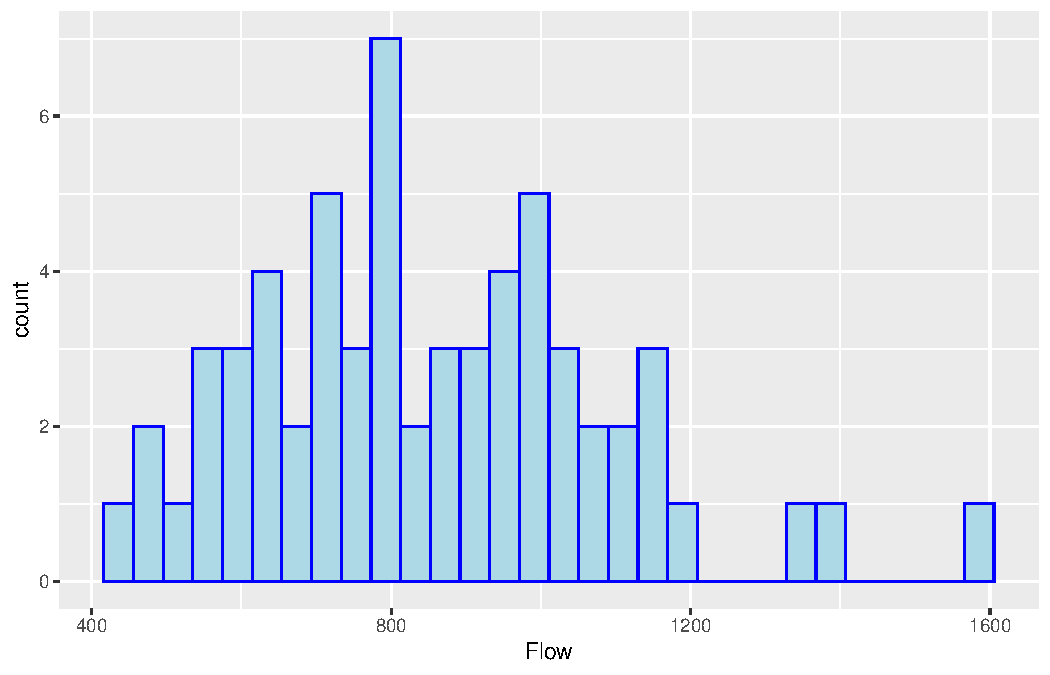
\includegraphics{IntroR_files/figure-latex/unnamed-chunk-189-1} \end{center}

No comando existem dois tipos de informação, separadas pelo símbolo \(+\). Este símbolo marca o fim de uma camada e início da outra. No \texttt{ggplot()} cada camada adiciona um elemento novo ou formata um elemento existente no gráfico. A ordem em que as camadas são inseridas raramente importa, ainda que seja interessante inserí-las de modo que facilite a leitura do código. No exemplo acima temos as camadas gedaras por:

\begin{itemize}
\tightlist
\item
  \texttt{ggplot()}: esta função mostra um argumento \texttt{data\ =}, onde informamos o nome do \texttt{data.frame} de onde serão lidos os dados (\emph{No ggplot, os dados sempre devem estar dispostos dentro de um data frame}). No segundo argumento \texttt{mapping\ =}, informamos sobre a \textbf{estética do gráfico}. Por hora, esta estética foi limitada a \texttt{aes(x\ =\ Flow)}, dizendo que nosso gráfico irá conter no eixo \texttt{x} a variável \texttt{Flow} do data frame.
\end{itemize}

Até este momento não definimos qual será o tipo gráfico.

\begin{itemize}
\tightlist
\item
  Na segunda camada estabelecemos a \textbf{geometria} do gráfico, neste caso composta por um histograma (\texttt{geom\_histogram}), onde a cor da borda foi definida por \texttt{color\ =\ "blue"} e o preenchimento por \texttt{fill\ =\ "lightblue"}.
\end{itemize}

Vamos adicionar algumas formatações adicionais:

\begin{Shaded}
\begin{Highlighting}[]
\FunctionTok{ggplot}\NormalTok{(}\AttributeTok{data =}\NormalTok{ hub, }\AttributeTok{mapping =} \FunctionTok{aes}\NormalTok{(}\AttributeTok{x =}\NormalTok{ Flow)) }\SpecialCharTok{+}
  \FunctionTok{geom\_histogram}\NormalTok{(}\AttributeTok{color =} \StringTok{"blue"}\NormalTok{, }\AttributeTok{fill =} \StringTok{"lightblue"}\NormalTok{) }\SpecialCharTok{+}
  \FunctionTok{labs}\NormalTok{(}\AttributeTok{title =} \StringTok{"Histograma de vazão do riacho Hubbard"}\NormalTok{, }
       \AttributeTok{x =} \FunctionTok{bquote}\NormalTok{(}\FunctionTok{Vazao}\NormalTok{ (m}\SpecialCharTok{\^{}}\DecValTok{3}\SpecialCharTok{/}\NormalTok{s)),}
       \AttributeTok{y =} \StringTok{"Contagem"}\NormalTok{) }\SpecialCharTok{+}
  \FunctionTok{theme}\NormalTok{(}\AttributeTok{plot.title =} \FunctionTok{element\_text}\NormalTok{(}\AttributeTok{hjust =} \FloatTok{0.5}\NormalTok{))}
\end{Highlighting}
\end{Shaded}

\begin{center}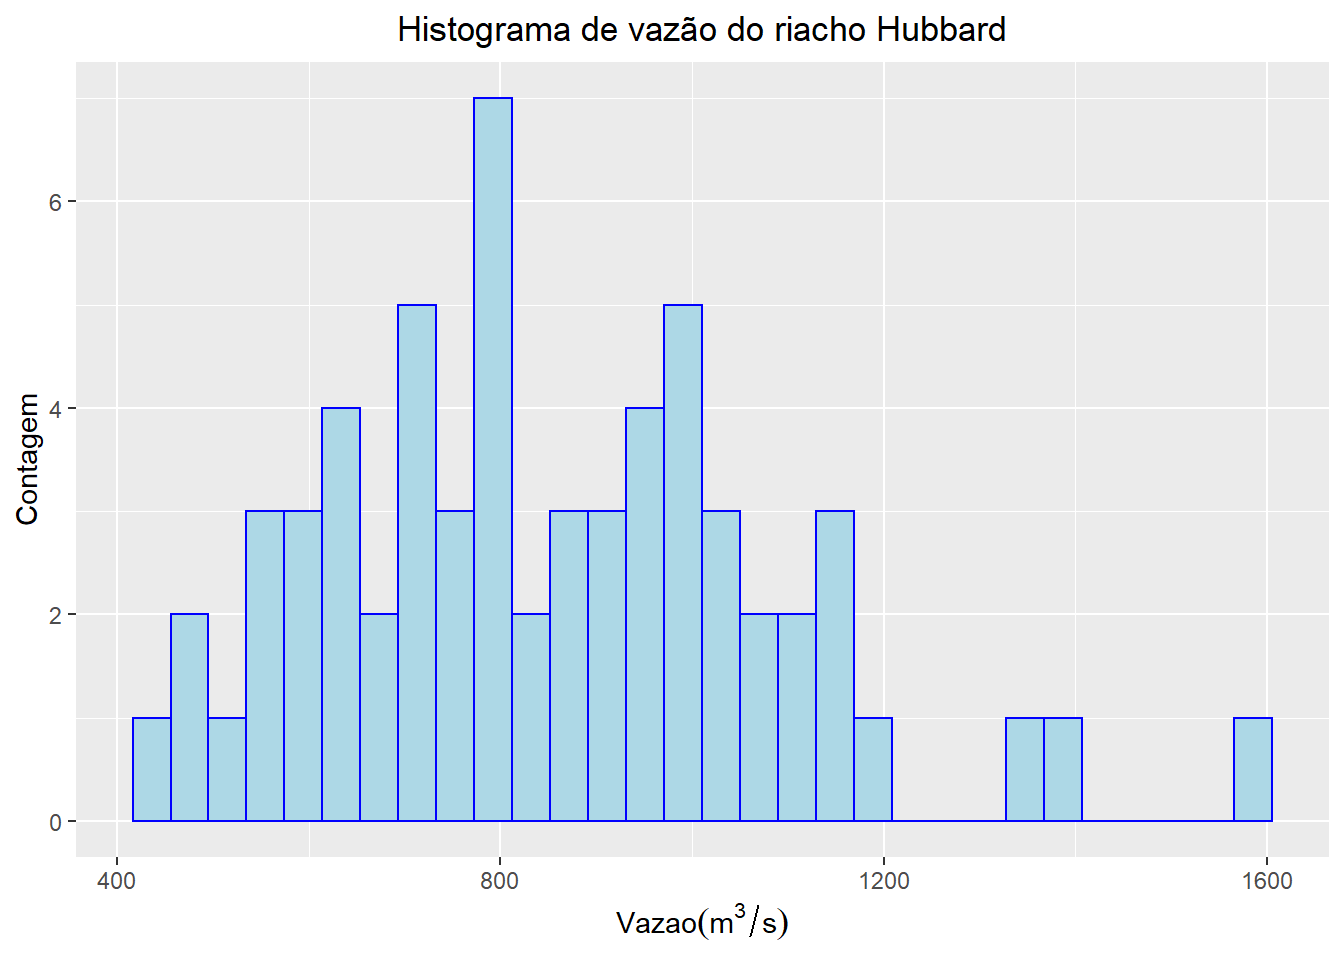
\includegraphics{IntroR_files/figure-latex/unnamed-chunk-190-1} \end{center}

Formatamos agora o \textbf{título}, os nomes dos eixos \texttt{x} e \texttt{y} e centralizamos o título (\texttt{theme(plot.title\ =\ element\_text(hjust\ =\ 0.5))}).

Embora possa parecer muita informação de uma única vez (e de fato é), o ponto é que você não precisará decorar nenhuma delas (mas se utilizar, acabará decorando!!). Uma simples busca por \href{https://www.google.com/search?sxsrf=ALeKk02h6lituhooE6EgHAVc2zcLsOWdLQ\%3A1594404890952\&ei=GrAIX5LrOciv5OUPnfGPsA0\&q=centralize+title+ggplot2\&oq=centralize+title+ggplot2\&gs_lcp=CgZwc3ktYWIQAzIECCMQJzoECAAQRzoHCCMQsAIQJ1CNDFjSPGDfRGgAcAF4AIABlgGIAfkIkgEDMC45mAEAoAEBqgEHZ3dzLXdpeg\&sclient=psy-ab\&ved=0ahUKEwiS4JyJpcPqAhXIF7kGHZ34A9YQ4dUDCAw\&uact=5}{centralize title ggplot2} te levará a estes comandos.

No histograma anterior, a vazão foi medida anualmente em trechos Deforested e em trechos Deforested. Vamos então adicionar esta variável à \emph{estética} (\texttt{aes()}) do gráfico, diferenciando os grupos em função da cor.

\begin{Shaded}
\begin{Highlighting}[]
\FunctionTok{ggplot}\NormalTok{(}\AttributeTok{data =}\NormalTok{ hub, }\AttributeTok{mapping =} \FunctionTok{aes}\NormalTok{(}\AttributeTok{x =}\NormalTok{ Flow, }\AttributeTok{color =}\NormalTok{ Treatment, }\AttributeTok{fill =}\NormalTok{ Treatment)) }\SpecialCharTok{+}
  \FunctionTok{geom\_histogram}\NormalTok{(}\AttributeTok{alpha =} \FloatTok{0.5}\NormalTok{)}
\end{Highlighting}
\end{Shaded}

\begin{center}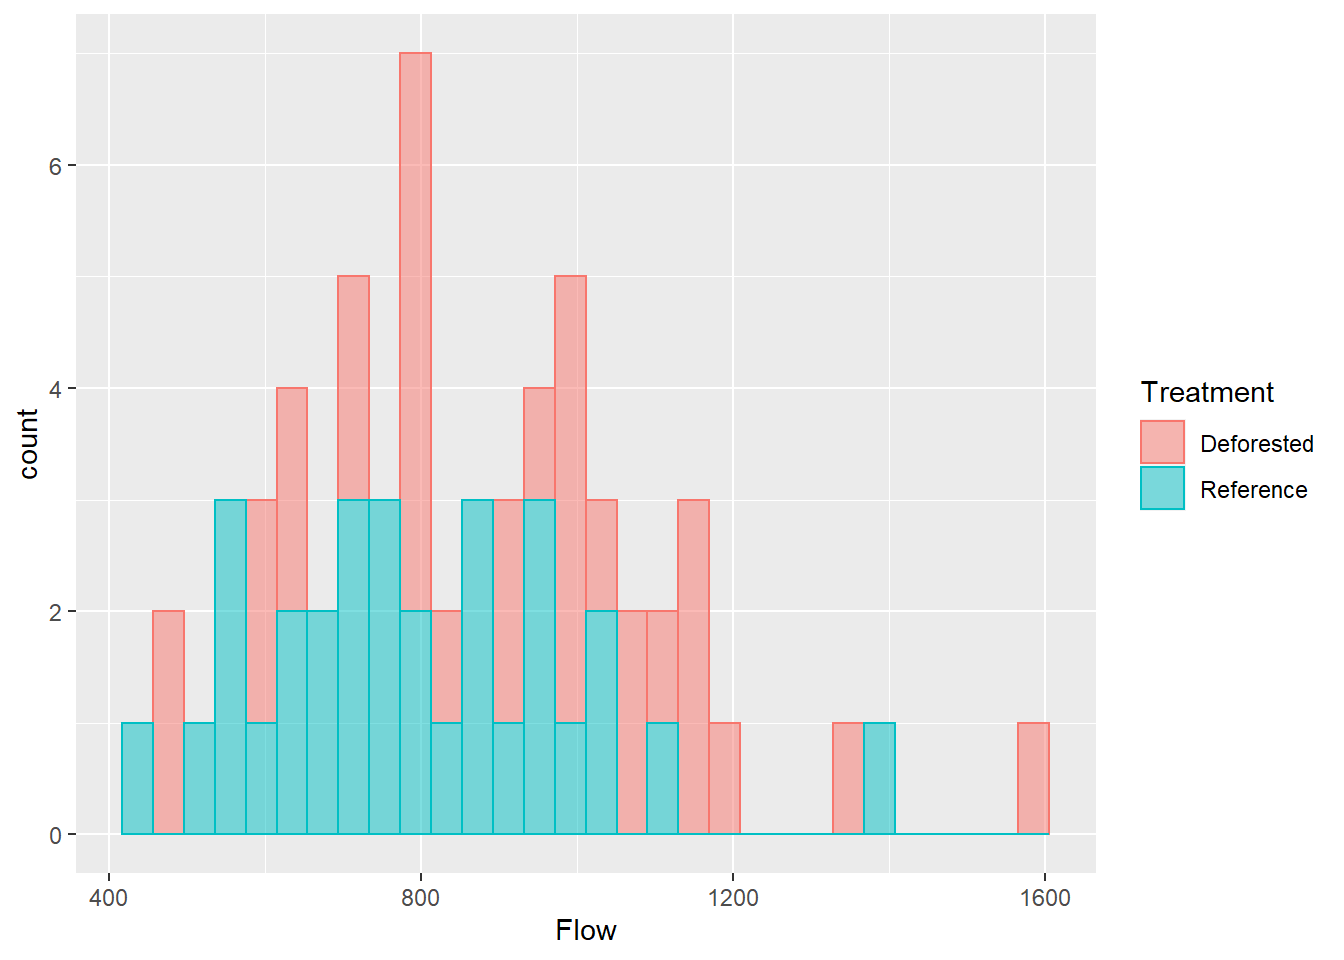
\includegraphics{IntroR_files/figure-latex/unnamed-chunk-191-1} \end{center}

\hypertarget{outras-geometrias-gruxe1ficas}{%
\subsection{\texorpdfstring{Outras \emph{Geometrias} gráficas}{Outras Geometrias gráficas}}\label{outras-geometrias-gruxe1ficas}}

Além dos histogramas temos muitas outras geometrias gráficas do tipo \texttt{geom\_NOME()}. Algumas muito utilizadas são:

\begin{itemize}
\tightlist
\item
  geom\_abline()
\item
  geom\_bar()
\item
  geom\_boxplot()
\item
  geom\_line()
\item
  geom\_point()
\item
  geom\_smooth()
\item
  geom\_text()
\end{itemize}

\hypertarget{guxe1fico-de-dispersuxe3o}{%
\section{Gáfico de dispersão}\label{guxe1fico-de-dispersuxe3o}}

\begin{Shaded}
\begin{Highlighting}[]
\FunctionTok{ggplot}\NormalTok{(}\AttributeTok{data =}\NormalTok{ hub, }\AttributeTok{mapping =} \FunctionTok{aes}\NormalTok{(}\AttributeTok{x =}\NormalTok{ Precipitation, }\AttributeTok{y =}\NormalTok{ Flow)) }\SpecialCharTok{+}
  \FunctionTok{geom\_point}\NormalTok{(}\AttributeTok{shape =} \DecValTok{21}\NormalTok{) }\SpecialCharTok{+}
  \FunctionTok{labs}\NormalTok{(}\AttributeTok{y =} \FunctionTok{bquote}\NormalTok{(Vazão (m}\SpecialCharTok{\^{}}\DecValTok{3}\SpecialCharTok{/}\NormalTok{s)),}
       \AttributeTok{x =} \FunctionTok{bquote}\NormalTok{(Precipitação (m}\SpecialCharTok{\^{}}\DecValTok{3}\SpecialCharTok{/}\NormalTok{ano)))}
\end{Highlighting}
\end{Shaded}

\begin{center}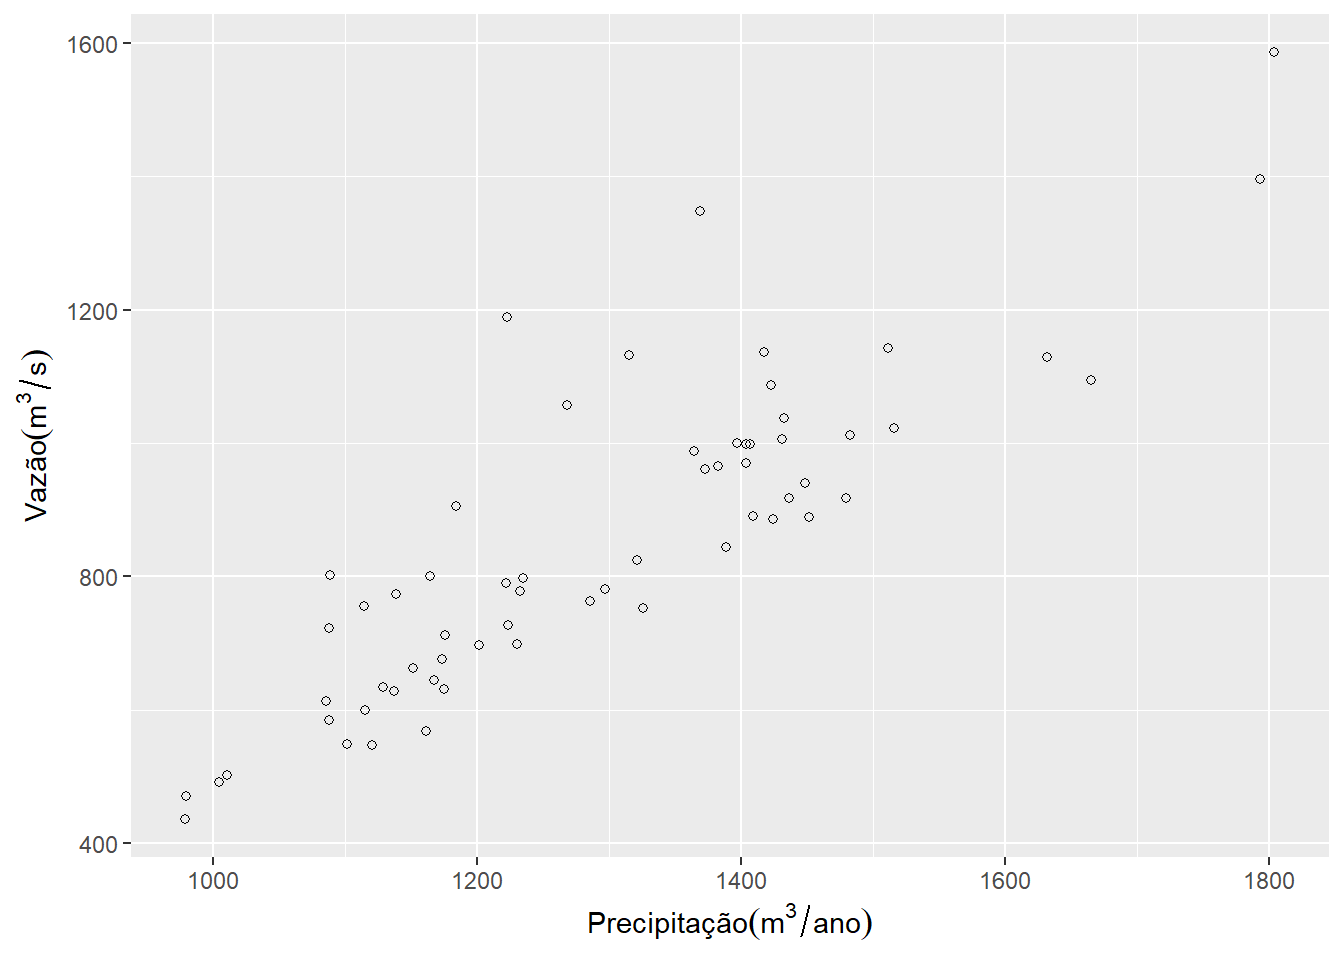
\includegraphics{IntroR_files/figure-latex/unnamed-chunk-192-1} \end{center}

Adicionando o \texttt{Treatment} à cor do gráfico e formatando a legenda.

\begin{Shaded}
\begin{Highlighting}[]
\FunctionTok{ggplot}\NormalTok{(}\AttributeTok{data =}\NormalTok{ hub, }\AttributeTok{mapping =} \FunctionTok{aes}\NormalTok{(}\AttributeTok{x =}\NormalTok{ Precipitation, }\AttributeTok{y =}\NormalTok{ Flow, }\AttributeTok{fill =}\NormalTok{ Treatment)) }\SpecialCharTok{+}
  \FunctionTok{geom\_point}\NormalTok{(}\AttributeTok{shape =} \DecValTok{21}\NormalTok{, }\AttributeTok{size =} \DecValTok{3}\NormalTok{) }\SpecialCharTok{+}
  \FunctionTok{labs}\NormalTok{(}\AttributeTok{y =} \FunctionTok{bquote}\NormalTok{(Vazão (m}\SpecialCharTok{\^{}}\DecValTok{3}\SpecialCharTok{/}\NormalTok{s)),}
       \AttributeTok{x =} \FunctionTok{bquote}\NormalTok{(Precipitação (m}\SpecialCharTok{\^{}}\DecValTok{3}\SpecialCharTok{/}\NormalTok{ano))) }\SpecialCharTok{+}
  \FunctionTok{guides}\NormalTok{(}\AttributeTok{fill=}\FunctionTok{guide\_legend}\NormalTok{(}\AttributeTok{title=}\StringTok{"Estado da área"}\NormalTok{)) }\SpecialCharTok{+}
  \FunctionTok{scale\_fill\_manual}\NormalTok{(}\AttributeTok{values =} \FunctionTok{c}\NormalTok{(}\StringTok{"blue"}\NormalTok{, }\StringTok{"yellow"}\NormalTok{))}
\end{Highlighting}
\end{Shaded}

\begin{center}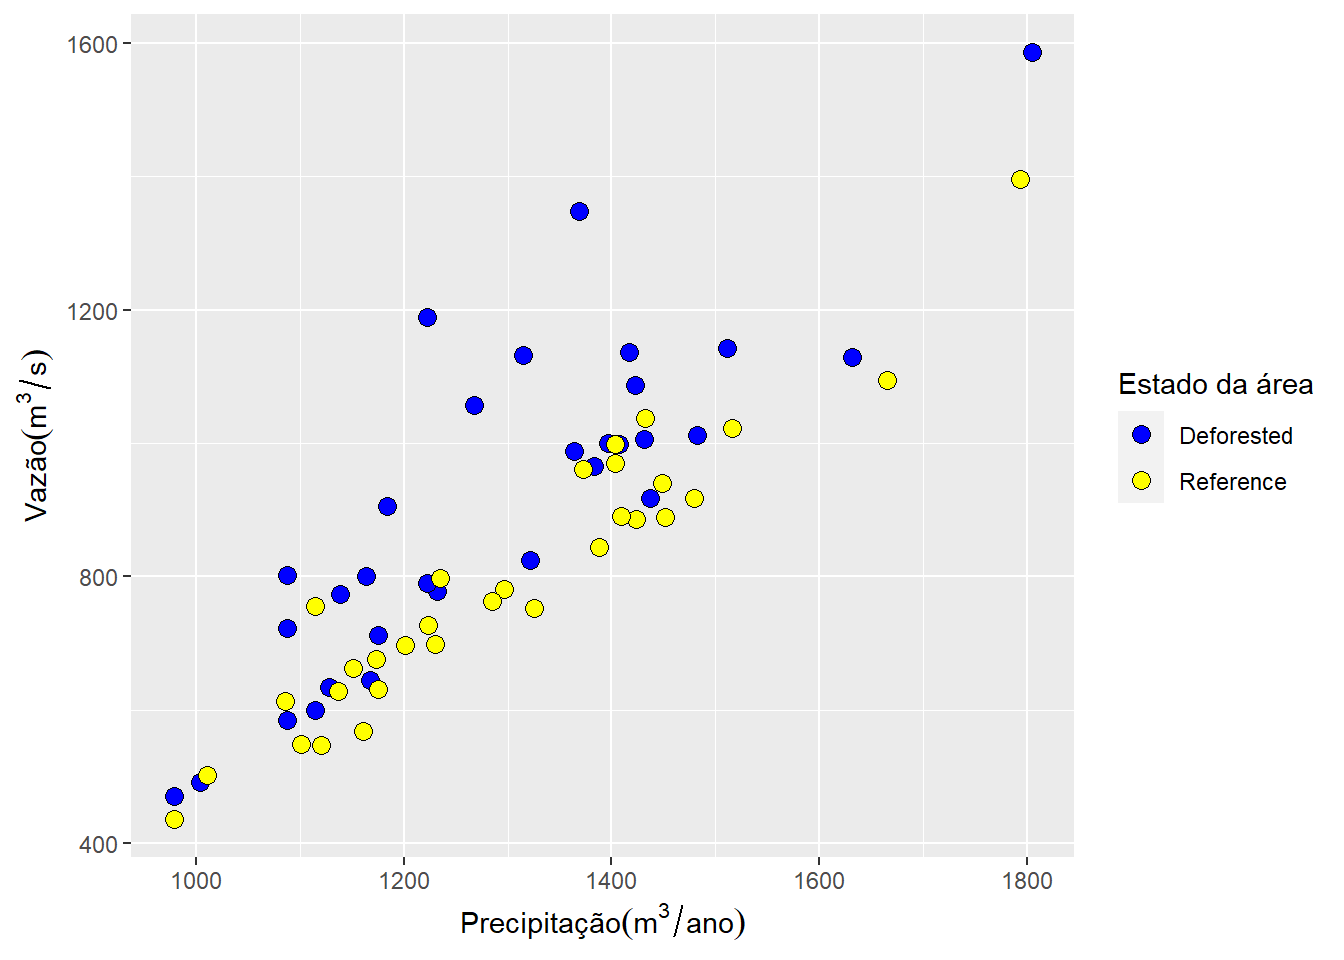
\includegraphics{IntroR_files/figure-latex/unnamed-chunk-193-1} \end{center}

Adicionando um texto com informação do Ano de mensuração.

\begin{Shaded}
\begin{Highlighting}[]
\FunctionTok{ggplot}\NormalTok{(}\AttributeTok{data =}\NormalTok{ hub, }\AttributeTok{mapping =} \FunctionTok{aes}\NormalTok{(}\AttributeTok{x =}\NormalTok{ Precipitation, }\AttributeTok{y =}\NormalTok{ Flow, }\AttributeTok{label =}\NormalTok{ Year}
\NormalTok{                                 , }\AttributeTok{color =}\NormalTok{ Treatment)) }\SpecialCharTok{+}
  \FunctionTok{geom\_text}\NormalTok{(}\AttributeTok{size =} \DecValTok{3}\NormalTok{) }\SpecialCharTok{+}
  \FunctionTok{labs}\NormalTok{(}\AttributeTok{y =} \FunctionTok{bquote}\NormalTok{(Vazão (m}\SpecialCharTok{\^{}}\DecValTok{3}\SpecialCharTok{/}\NormalTok{s)),}
       \AttributeTok{x =} \FunctionTok{bquote}\NormalTok{(Precipitação (m}\SpecialCharTok{\^{}}\DecValTok{3}\SpecialCharTok{/}\NormalTok{ano))) }\SpecialCharTok{+}
  \FunctionTok{guides}\NormalTok{(}\AttributeTok{color=}\FunctionTok{guide\_legend}\NormalTok{(}\AttributeTok{title=}\StringTok{"Estado da área"}\NormalTok{)) }\SpecialCharTok{+}
  \FunctionTok{scale\_color\_manual}\NormalTok{(}\AttributeTok{values =} \FunctionTok{c}\NormalTok{(}\StringTok{"blue"}\NormalTok{, }\StringTok{"red"}\NormalTok{))}
\end{Highlighting}
\end{Shaded}

\begin{center}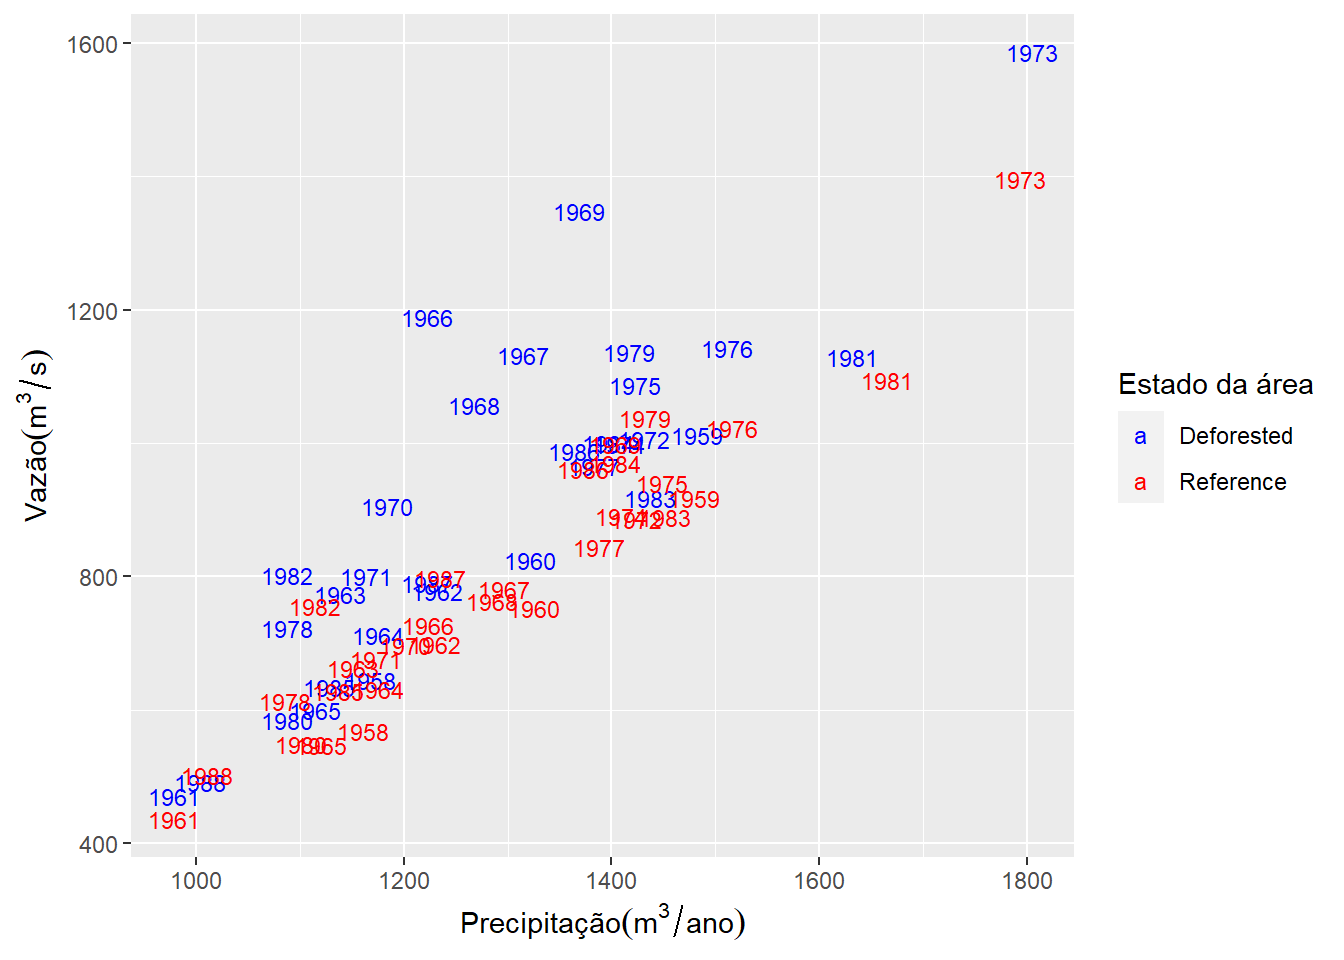
\includegraphics{IntroR_files/figure-latex/unnamed-chunk-194-1} \end{center}

\hypertarget{boxplot-2}{%
\section{Boxplot}\label{boxplot-2}}

\begin{Shaded}
\begin{Highlighting}[]
\FunctionTok{ggplot}\NormalTok{(}\AttributeTok{data =}\NormalTok{ hub, }\AttributeTok{mapping =} \FunctionTok{aes}\NormalTok{(}\AttributeTok{x =}\NormalTok{ Treatment, }\AttributeTok{y =}\NormalTok{ Flow)) }\SpecialCharTok{+}
  \FunctionTok{geom\_boxplot}\NormalTok{() }\SpecialCharTok{+}
  \FunctionTok{labs}\NormalTok{(}\AttributeTok{y =} \FunctionTok{bquote}\NormalTok{(Vazão (m}\SpecialCharTok{\^{}}\DecValTok{3}\SpecialCharTok{/}\NormalTok{s)),}
       \AttributeTok{x =} \StringTok{""}\NormalTok{)}
\end{Highlighting}
\end{Shaded}

\begin{center}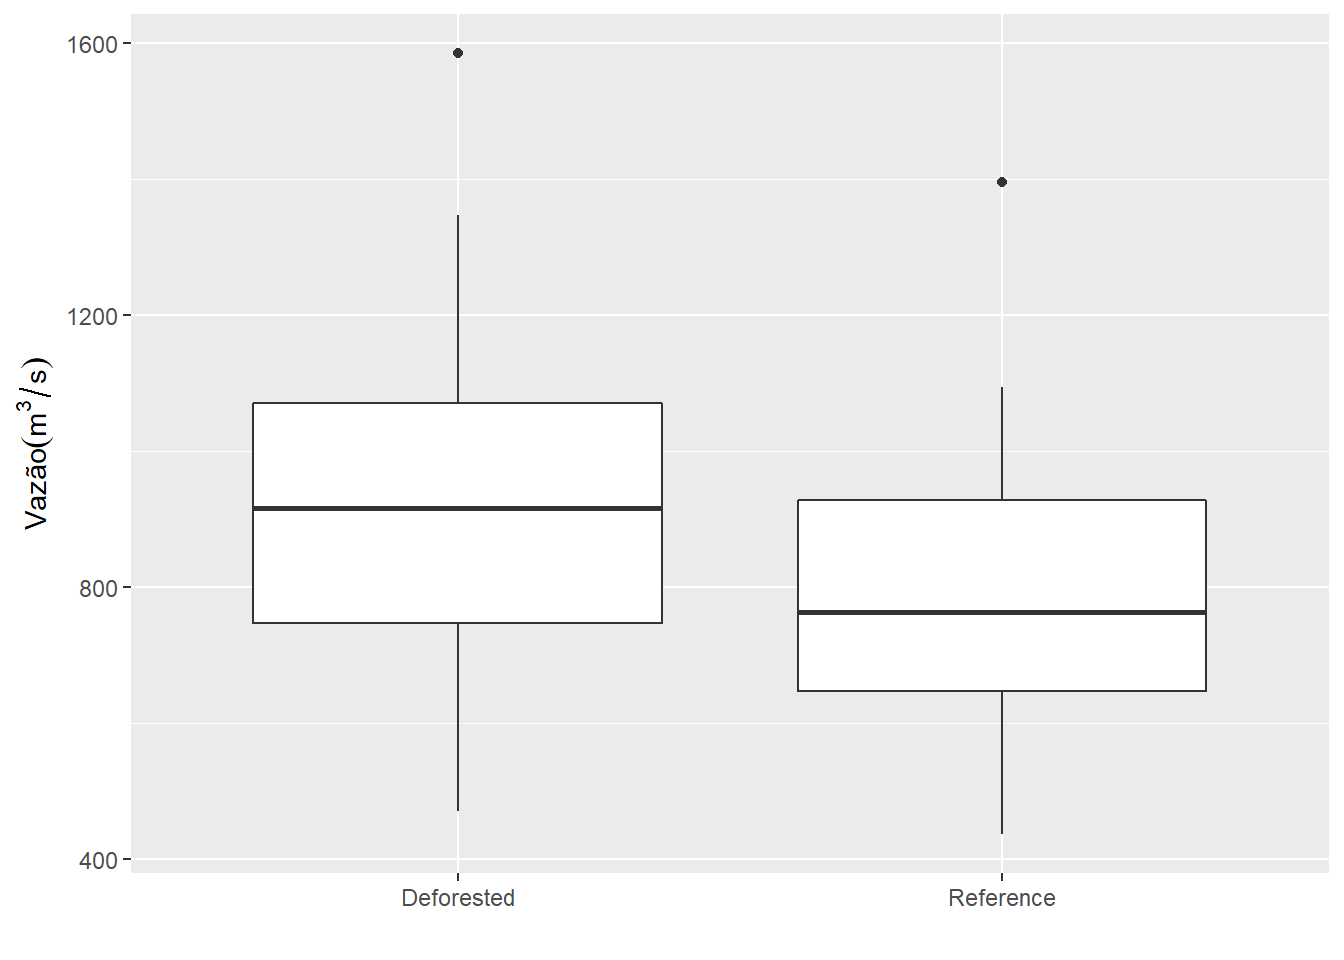
\includegraphics{IntroR_files/figure-latex/unnamed-chunk-195-1} \end{center}

Vamos inverter a ordem dos boxplots.

\begin{Shaded}
\begin{Highlighting}[]
\FunctionTok{ggplot}\NormalTok{(}\AttributeTok{data =}\NormalTok{ hub, }\AttributeTok{mapping =} \FunctionTok{aes}\NormalTok{(}\AttributeTok{x =}\NormalTok{ Treatment, }\AttributeTok{y =}\NormalTok{ Flow)) }\SpecialCharTok{+}
  \FunctionTok{geom\_boxplot}\NormalTok{() }\SpecialCharTok{+}
  \FunctionTok{labs}\NormalTok{(}\AttributeTok{y =} \FunctionTok{bquote}\NormalTok{(Vazão (m}\SpecialCharTok{\^{}}\DecValTok{3}\SpecialCharTok{/}\NormalTok{s)),}
       \AttributeTok{x =} \StringTok{""}\NormalTok{) }\SpecialCharTok{+}
  \FunctionTok{scale\_x\_discrete}\NormalTok{(}
    \AttributeTok{limits =} \FunctionTok{c}\NormalTok{(}\StringTok{"Reference"}\NormalTok{, }\StringTok{"Deforested"}\NormalTok{))}
\end{Highlighting}
\end{Shaded}

\begin{center}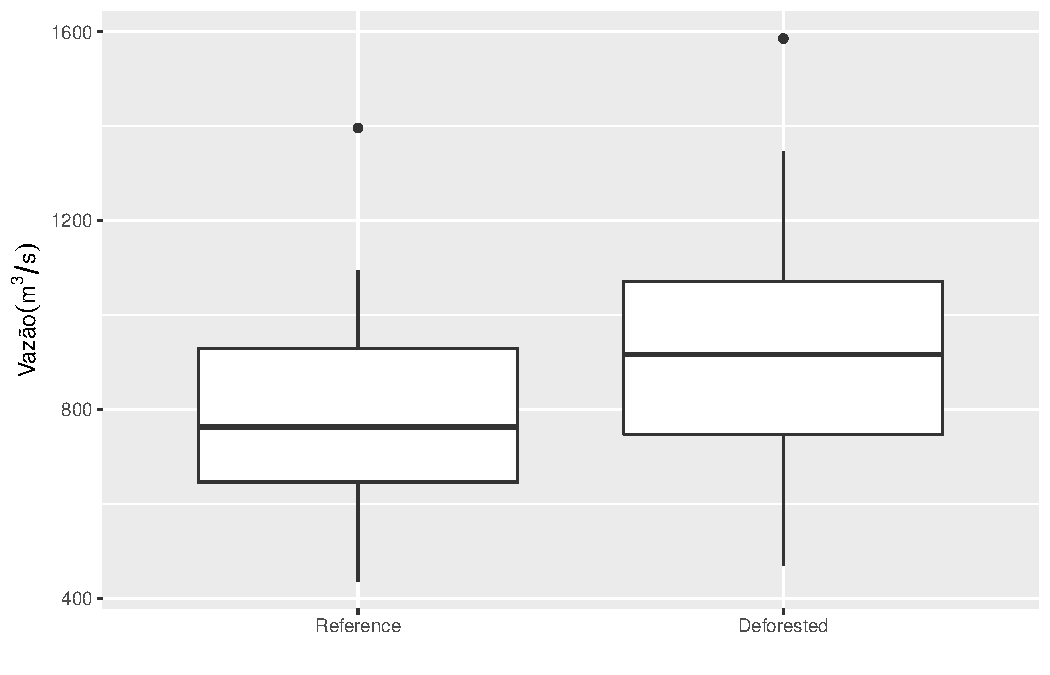
\includegraphics{IntroR_files/figure-latex/unnamed-chunk-196-1} \end{center}

\hypertarget{gruxe1fico-de-linhas}{%
\section{Gráfico de linhas}\label{gruxe1fico-de-linhas}}

\begin{Shaded}
\begin{Highlighting}[]
\NormalTok{hub }\SpecialCharTok{\%\textgreater{}\%} 
  \FunctionTok{filter}\NormalTok{(Treatment }\SpecialCharTok{==} \StringTok{"Deforested"}\NormalTok{) }\SpecialCharTok{\%\textgreater{}\%} 
  \FunctionTok{ggplot}\NormalTok{(}\AttributeTok{mapping =} \FunctionTok{aes}\NormalTok{(}\AttributeTok{x =}\NormalTok{ Year, }\AttributeTok{y =}\NormalTok{ Flow)) }\SpecialCharTok{+}
    \FunctionTok{geom\_line}\NormalTok{() }\SpecialCharTok{+}
    \FunctionTok{labs}\NormalTok{(}\AttributeTok{y =} \FunctionTok{bquote}\NormalTok{(Vazão (m}\SpecialCharTok{\^{}}\DecValTok{3}\SpecialCharTok{/}\NormalTok{s)),}
         \AttributeTok{x =} \StringTok{"Ano"}\NormalTok{)}
\end{Highlighting}
\end{Shaded}

\begin{center}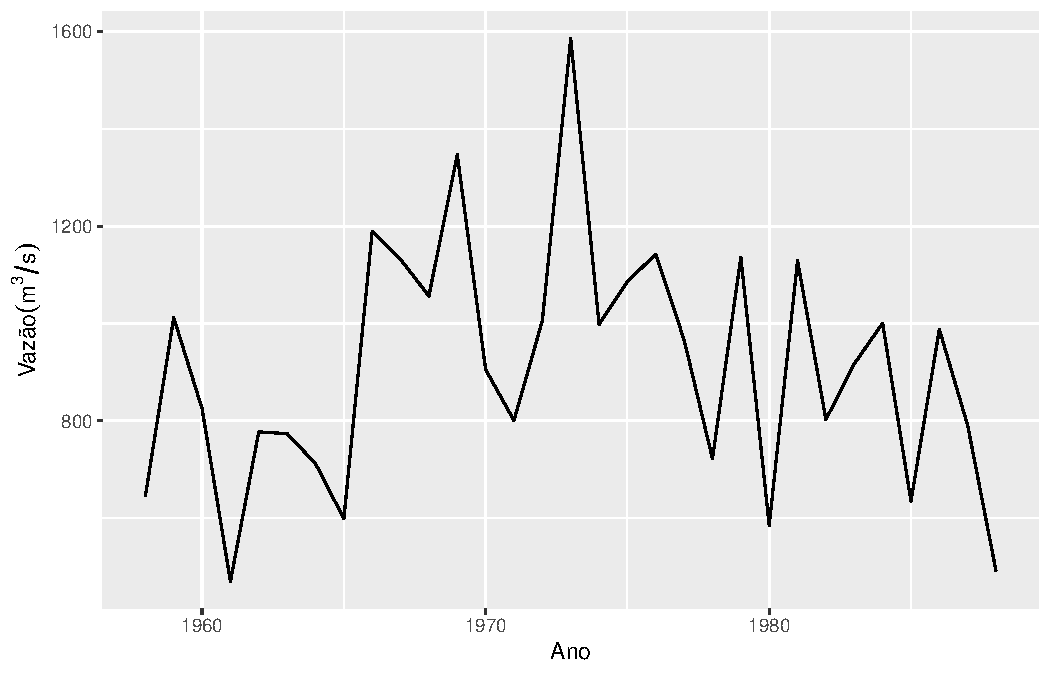
\includegraphics{IntroR_files/figure-latex/unnamed-chunk-197-1} \end{center}

Na figura, utilizamos o operador \textbf{pipe}, e a função \texttt{filter()} para extrair somente as linhas do riacho desmatado. Vamos adicionar os dois riachos.

\begin{Shaded}
\begin{Highlighting}[]
\FunctionTok{ggplot}\NormalTok{(hub, }\AttributeTok{mapping =} \FunctionTok{aes}\NormalTok{(}\AttributeTok{x =}\NormalTok{ Year, }\AttributeTok{y =}\NormalTok{ Flow, }\AttributeTok{color =}\NormalTok{ Treatment)) }\SpecialCharTok{+}
  \FunctionTok{geom\_line}\NormalTok{() }\SpecialCharTok{+}
  \FunctionTok{labs}\NormalTok{(}\AttributeTok{y =} \FunctionTok{bquote}\NormalTok{(Vazão (m}\SpecialCharTok{\^{}}\DecValTok{3}\SpecialCharTok{/}\NormalTok{s)),}
         \AttributeTok{x =} \StringTok{"Ano"}\NormalTok{)}
\end{Highlighting}
\end{Shaded}

\begin{center}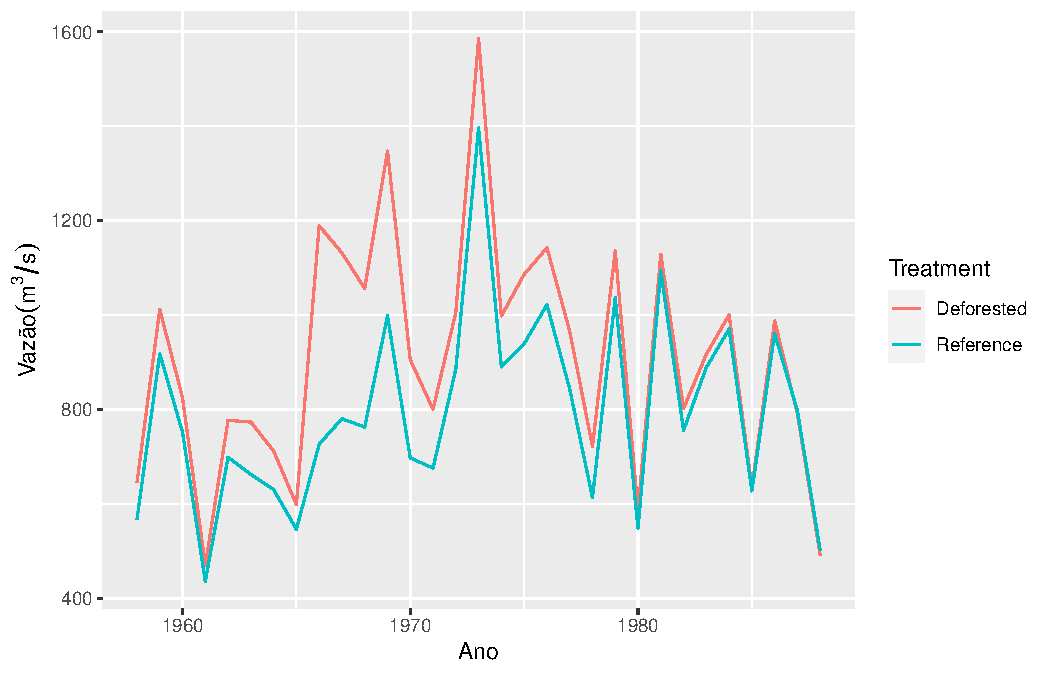
\includegraphics{IntroR_files/figure-latex/unnamed-chunk-198-1} \end{center}

\hypertarget{gruxe1fico-de-barras-2}{%
\section{Gráfico de barras}\label{gruxe1fico-de-barras-2}}

Vamos criar uma variável categórica \texttt{Vazao\_cat} contendo os níveis \texttt{Extrema} (se \texttt{Flow} \(>= 1000 m^3/s\)) e \texttt{Normal} caso contrário. Em seguida vamos contar o número de observações com vazão extrema.

\begin{Shaded}
\begin{Highlighting}[]
\NormalTok{extremo }\OtherTok{\textless{}{-}} \DecValTok{1000}

\NormalTok{hub }\SpecialCharTok{\%\textgreater{}\%} 
  \FunctionTok{mutate}\NormalTok{(}\AttributeTok{Vazao\_cat =} \FunctionTok{ifelse}\NormalTok{(Flow }\SpecialCharTok{\textgreater{}=}\NormalTok{ extremo, }
                            \AttributeTok{yes =} \StringTok{"Extrema"}\NormalTok{, }
                            \AttributeTok{no =} \StringTok{"Normal"}\NormalTok{)) }\SpecialCharTok{\%\textgreater{}\%} 
  \FunctionTok{ggplot}\NormalTok{(}\AttributeTok{mapping =} \FunctionTok{aes}\NormalTok{(}\AttributeTok{x =}\NormalTok{ Vazao\_cat)) }\SpecialCharTok{+}
  \FunctionTok{geom\_bar}\NormalTok{()}
\end{Highlighting}
\end{Shaded}

\begin{center}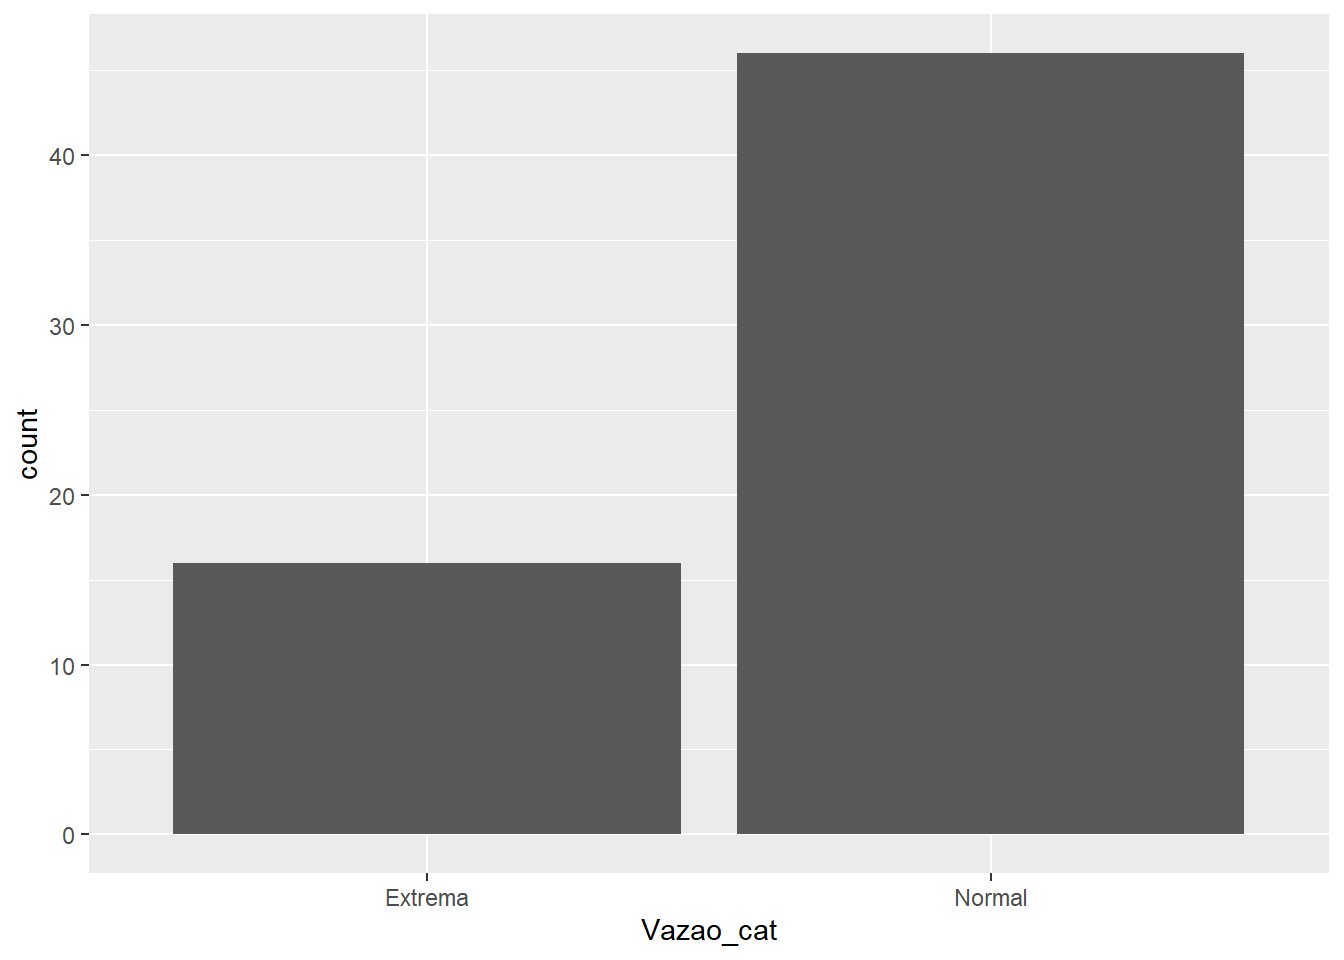
\includegraphics{IntroR_files/figure-latex/unnamed-chunk-199-1} \end{center}

Se dissermos que a variável está em \texttt{y} (\texttt{aes(y\ =\ Vazao\_cat)}) o gráfico fica na horizontal.

\begin{Shaded}
\begin{Highlighting}[]
\NormalTok{hub }\SpecialCharTok{\%\textgreater{}\%} 
  \FunctionTok{mutate}\NormalTok{(}\AttributeTok{Vazao\_cat =} \FunctionTok{ifelse}\NormalTok{(Flow }\SpecialCharTok{\textgreater{}=}\NormalTok{ extremo, }\AttributeTok{yes =} \StringTok{"Extrema"}\NormalTok{, }\AttributeTok{no =} \StringTok{"Normal"}\NormalTok{)) }\SpecialCharTok{\%\textgreater{}\%} 
  \FunctionTok{ggplot}\NormalTok{(}\AttributeTok{mapping =} \FunctionTok{aes}\NormalTok{(}\AttributeTok{y =}\NormalTok{ Vazao\_cat)) }\SpecialCharTok{+}
  \FunctionTok{geom\_bar}\NormalTok{()}
\end{Highlighting}
\end{Shaded}

\begin{center}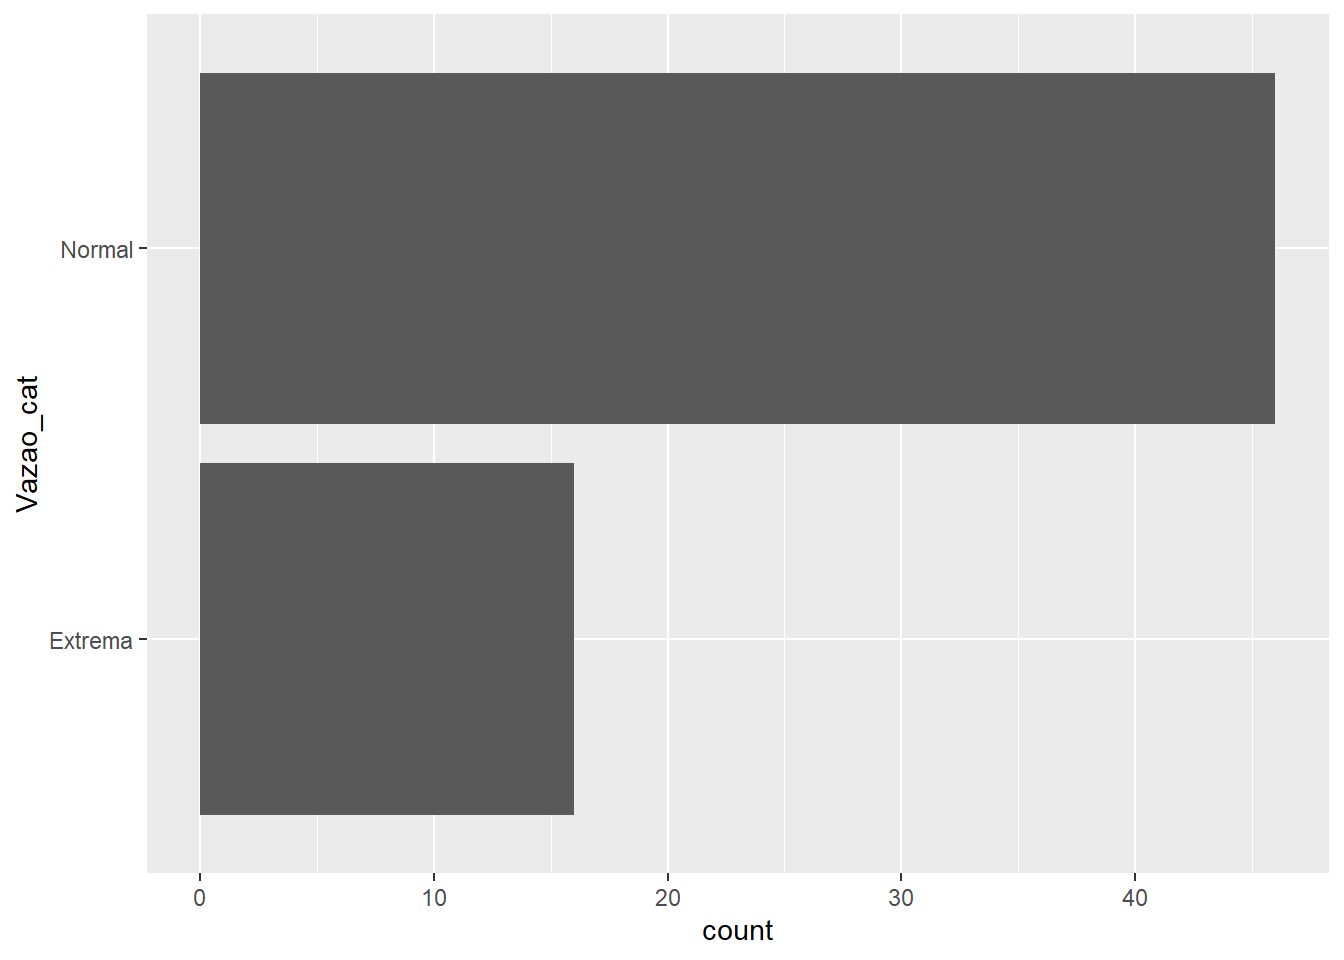
\includegraphics{IntroR_files/figure-latex/unnamed-chunk-200-1} \end{center}

\hypertarget{temas-no-ggplot2}{%
\section{\texorpdfstring{Temas no \texttt{ggplot2}}{Temas no ggplot2}}\label{temas-no-ggplot2}}

Embora possamos formatar todos os elementos gráficos, o \texttt{ggplot2} vem com temas pré-formatados que facilita este processo. Vejamos alguns. Para escolher um tema adicionamos uma camada com seu nome (\texttt{theme\_NOME()}). Veja o exemplo:

\begin{Shaded}
\begin{Highlighting}[]
\FunctionTok{ggplot}\NormalTok{(hub, }\AttributeTok{mapping =} \FunctionTok{aes}\NormalTok{(}\AttributeTok{x =}\NormalTok{ Year, }\AttributeTok{y =}\NormalTok{ Flow, }\AttributeTok{color =}\NormalTok{ Treatment)) }\SpecialCharTok{+}
  \FunctionTok{geom\_line}\NormalTok{() }\SpecialCharTok{+}
  \FunctionTok{theme\_classic}\NormalTok{()}
\end{Highlighting}
\end{Shaded}

\begin{center}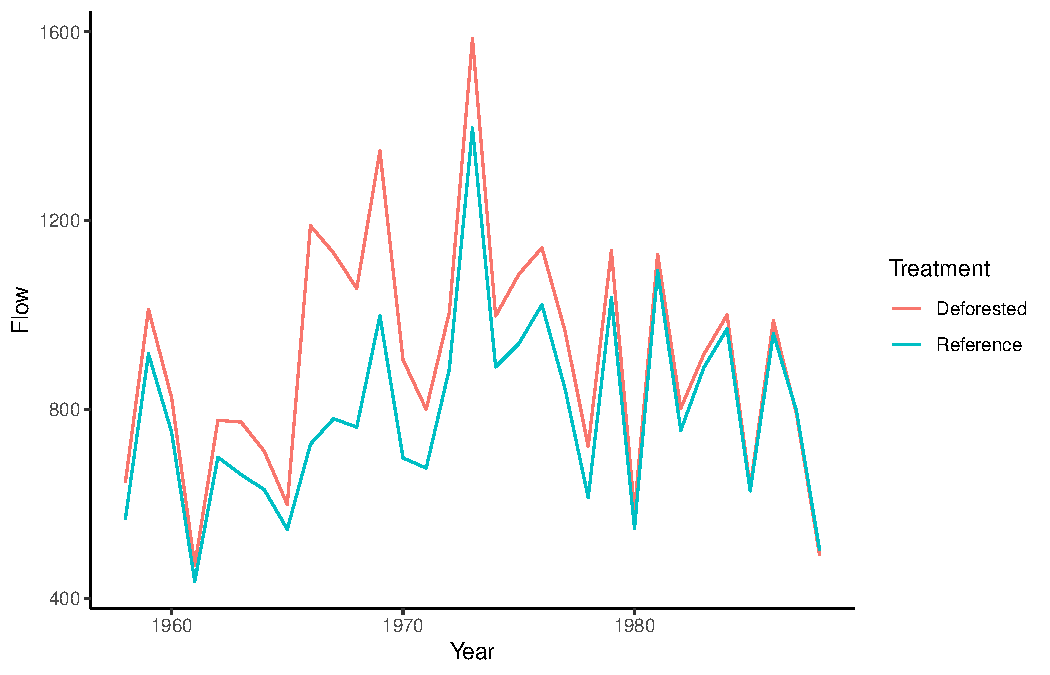
\includegraphics{IntroR_files/figure-latex/unnamed-chunk-201-1} \end{center}

Os temas básicos estão exemplificados abaixo. Além destes, o pacote \href{https://cran.r-project.org/web/packages/ggthemes/index.html}{\texttt{ggthemes}} oferece uma extensa variedade de outras formatações.

\begin{center}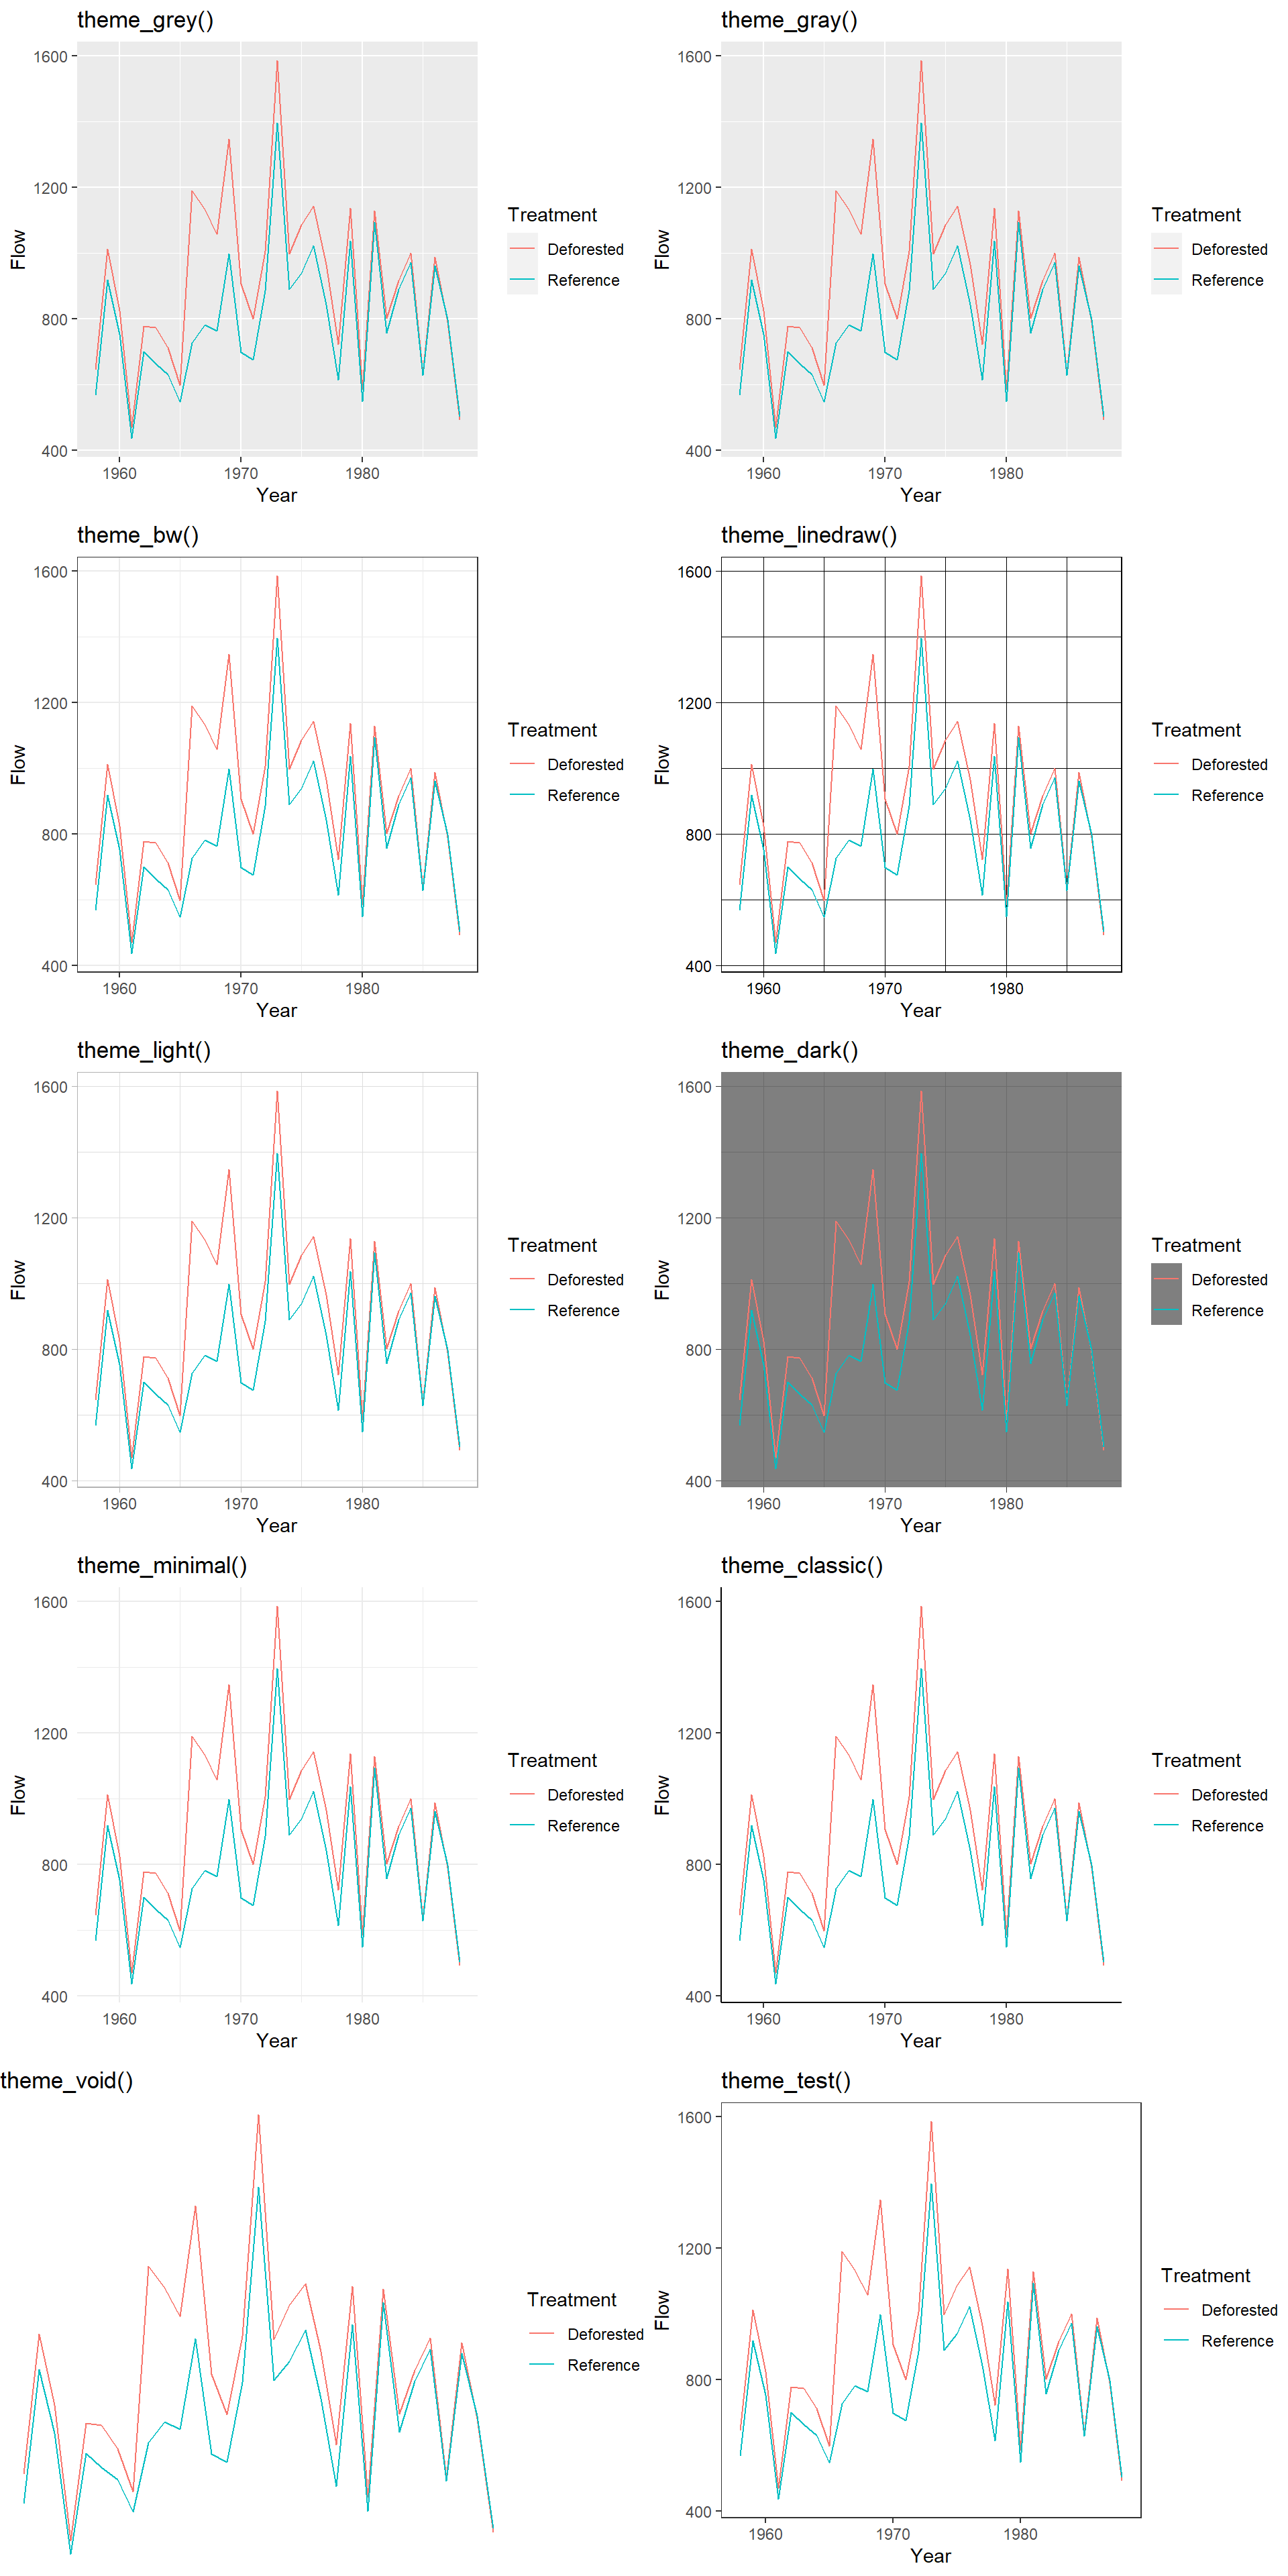
\includegraphics{IntroR_files/figure-latex/unnamed-chunk-202-1} \end{center}

\hypertarget{salvando-uma-figura-gerada-pelo-gglot2.}{%
\section{\texorpdfstring{Salvando uma figura gerada pelo \texttt{gglot2}.}{Salvando uma figura gerada pelo gglot2.}}\label{salvando-uma-figura-gerada-pelo-gglot2.}}

Uma forma simples de salvar um gráfico gerados pelo \texttt{gglot2} é utilizando a função \href{https://ggplot2.tidyverse.org/reference/ggsave.html}{\texttt{ggsave()}}.

\begin{Shaded}
\begin{Highlighting}[]
\FunctionTok{ggplot}\NormalTok{(hub, }\AttributeTok{mapping =} \FunctionTok{aes}\NormalTok{(}\AttributeTok{x =}\NormalTok{ Year, }\AttributeTok{y =}\NormalTok{ Flow, }\AttributeTok{color =}\NormalTok{ Treatment)) }\SpecialCharTok{+}
  \FunctionTok{geom\_line}\NormalTok{() }\SpecialCharTok{+}
  \FunctionTok{theme\_classic}\NormalTok{()}

\FunctionTok{ggsave}\NormalTok{(}\AttributeTok{filename =} \StringTok{"Exemplo\_ggsave.png"}\NormalTok{, }
       \AttributeTok{device =} \StringTok{"png"}\NormalTok{,}
       \AttributeTok{width =} \DecValTok{20}\NormalTok{, }
       \AttributeTok{height =} \DecValTok{20}\NormalTok{,}
       \AttributeTok{units =} \StringTok{"cm"}\NormalTok{,}
       \AttributeTok{dpi =} \DecValTok{480}\NormalTok{)  }
\end{Highlighting}
\end{Shaded}

\begin{center}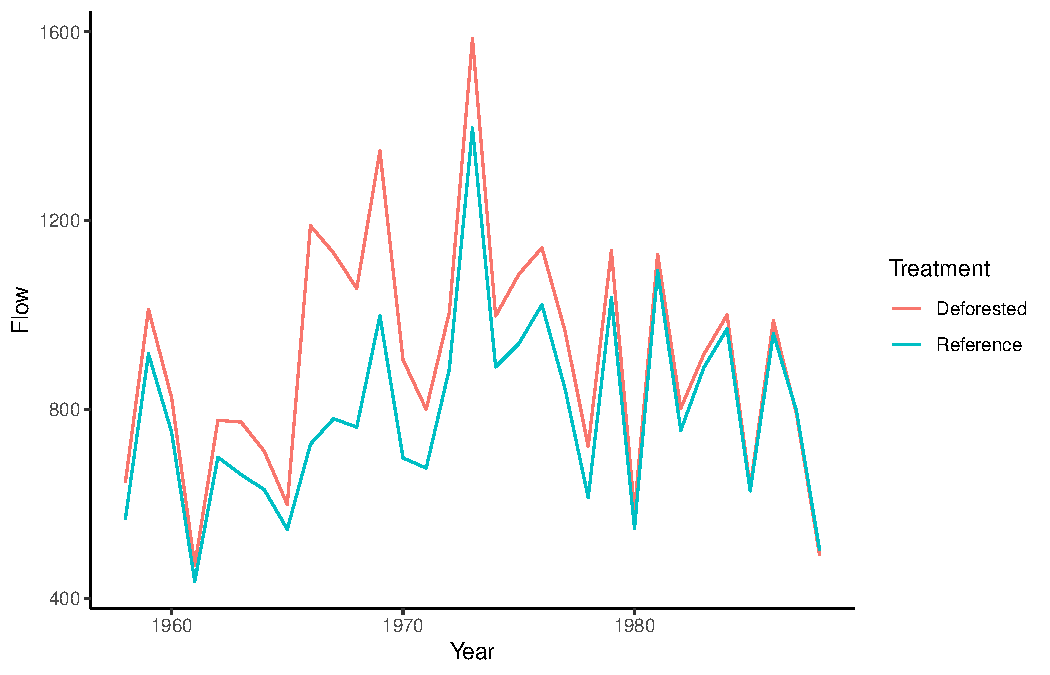
\includegraphics{IntroR_files/figure-latex/unnamed-chunk-204-1} \end{center}

Por padrão a função \texttt{ggsave()} salva o ultimo gráfico criado. Porém se existe um objeto salvo, você pode especificá-lo com o argumento \texttt{plot\ =\ objeto\_grafico}.

  \bibliography{book.bib,packages.bib}

\end{document}
